\chapter{辐射通量方案}
%\addcontentsline{toc}{chapter}{辐射通量方案}
%\begin{辐射通量方案}

\begin{mymdframed}{代码}
章节~\ref{sec:土壤反照率} -- \ref{sec:改进的二流近似植被辐射传输模型} 对应的代码文件为\texttt{MOD\_Albedo.F90}。
\end{mymdframed}


\section{土壤反照率}\label{sec:土壤反照率}
土壤反照率采用陆面模式BATS方案 \citep{dickinson1986biosphere,dickinson1993biosphere},利用土壤颜色和土壤表层含水量计算得到,公式如下:
\begin{equation}\label{eq:soil_albedo1}
\alpha_{soi,vis,dir}=\alpha_{soi,vis,dif}=\min\left(\alpha_{sat, vis}+\max\left(0,0.11-0.40 \theta_{l}\right), \alpha_{dry, vis}\right)
\end{equation}
%
\begin{equation}
\alpha_{soi,nir,dir}=\alpha_{soi,nir,dif}=\min\left(\alpha_{sat, nir}+\max\left(0,0.11-0.40 \theta_{l}\right), \alpha_{dry, nir}\right)
\end{equation}
其中$\alpha$表示反照率,下标$soi$表示土壤,$vis$和$nir$分别表示可见光(<0.7µm)和近红外波段(>0.7µm),$dir$($dif$)表示直射光(漫射光),$\alpha_{sat}$和$\alpha_{dry}$是根据土壤颜色分类,通过查找表得到的饱和($sat$)和干($dry$)土壤的反照率数值,$\theta_{l}$为表层(即第一层)土壤体积含水量。以上土壤反照率的计算适用于植被(土壤)、湿地次网格,当城市模式未打开时,同样用于城市地区。目前土壤颜色数据采用CLM 4.5,全球20种颜色分类数据,包括干土和湿土的可见光波段和近红外波段。漫射光与直射光相应波段反射率查找表数值一致。该查找表是\citet{lawrence2007representing}通过二流近似植被辐射传输模型与卫星遥感观测反照率拟合得到。


\section{永久性冰川反照率}\label{sec:永久性冰川反照率}
对于永久性冰川覆盖地表,简单将可见光波段反照率设置为0.8,近红外波段设置为0.55,直射光与漫射光一致,即:
\begin{equation}
\alpha_{ice,vis,dir}=\alpha_{ice,vis,dif}=0.8
\end{equation}
%
\begin{equation}
\alpha_{ice,nir,dir}=\alpha_{ice,nir,dif}=0.55
\end{equation}

\section{内陆水体反照率}
对于液态水和直射入射辐射,反照率为太阳天顶角余弦值$\mu$的函数,计算为$\frac{0.05}{\mu+0.15}$;漫射入射辐射时,设置为常数0.1,可见光与近红外波段一致,即:
%
\begin{equation}
\alpha_{wat,vis,dir}=\alpha_{wat,nir,dir}= \frac {0.05}{\mu+0.15}
\end{equation}
%
\begin{equation}
\alpha_{wat,vis,dif}=\alpha_{wat,nir,dif}=0.1
\end{equation}

当水体结冰,即水体表面温度小于273.16 K时,可见光波段反照率设置为0.6,近红外波段设置为0.4,直射光与漫射光一致:
%
\begin{equation}
\alpha_{wat,vis,dir}=\alpha_{wat,vis,dif}=0.6
\end{equation}
%
\begin{equation}
\alpha_{wat,nir,dir}=\alpha_{wat,nir,dif}=0.4
\end{equation}

\section{积雪反照率}

CoLM提供两种积雪反照率方案可供选择:1) BATS积雪反照率方案(章节~\ref{BATS积雪反照率});2) SNICAR积雪反照率方案(章节~\ref{SNICAR积雪反照率})。

\subsection{BATS积雪反照率方案}\label{BATS积雪反照率}

CoLM2014以及之前版本采用 \citet{dickinson1986biosphere} BATS方案,当不打开SNICAR积雪反照率模块时采用,主要考虑太阳高度角和雪龄 (snow age) 两个主要参数,计算如下:
\begin{equation}
\alpha_{sno, vis, dir}=\alpha_{sno, vis, dif}+0.4 f(\mu)\left(1-\alpha_{sno, vis, dif}\right)
\end{equation}
%
\begin{equation}
\alpha_{sno,nir,dir}=\alpha_{sno, nir, dif}+0.4 f(\mu)\left(1-\alpha_{sno,nir,dif}\right)
\end{equation} 
%
\begin{equation}\label{alpha_sno_vis_dif}
\alpha_{sno,vis,dif}=0.85\left(1-0.2 F_{age}\right)
\end{equation}
%
\begin{equation}\label{alpha_sno_nir_dif}
\alpha_{sno,nir,dif}=0.65\left(1-0.5 F_{age}\right)
\end{equation}
其中下标$sno$表示雪盖地表,$f(\mu)$是一用来表征雪盖反照率与太阳高度角关系的参数化函数:
\begin{equation}\label{fmu}
f(\mu)=\max\left[0,\left(\frac{1.5}{1+4 \mu}-0.5\right)\right]
\end{equation}
公式~\eqref{alpha_sno_vis_dif}、\eqref{alpha_sno_nir_dif} 中0.85和0.65分别表示可见光和近红外波段新雪反照率,
$F_{age}$表示雪龄影响因子,使得雪的反照率随着雪盖中雪晶颗粒的增长和灰尘等杂质的积累而降低,其计算为:
\begin{equation}
F_{a g e}=\frac{\tau_{sno}}{1+\tau_{sno}}
\end{equation}
$\tau_{sno}$表示无量纲雪龄,是一预报变量,它随时间的变化函数为:
\begin{equation}
\Delta \tau_{sno}=1 \times 10^{-6}\left(r_{1}+r_{2}+r_{3}\right) \Delta t
\end{equation}
其中$\Delta t$是积分时间步长(s),
\begin{align}
r_{1} &= \exp \left[5000\left(\frac{1}{273.16}-\frac{1}{T_{g}}\right)\right] \\
%\end{equation}
%\begin{equation}
r_{2} &= r_{1}^{10} \leqslant 1 \\
%\end{equation}
%\begin{equation}
r_{3} &= 0.3
\end{align}
上式中,$r_1$表示雪盖中水汽的扩散后凝华导致的雪晶颗粒增长对反照率的影响,$r_2$表示融雪对反照率的影响,$r_3$表示灰尘或杂质的影响[注: BATS在南极$r_3$设置为0.01]。
为了考虑新的降雪影响,在$\tau_{sno}$的计算中还包含计算时间步长内的降雪量,表示为:
\begin{equation}
\tau_{sno}^{(N+1)}=\left(\tau_{sno}^{(N)}+\Delta \tau_{sno}\right)\left(1-100 \Delta p_{sno}\right)
\end{equation}
其中$\Delta p_{sno}$为在$t^{(N+1)}$-$t^{(N)}$时间内的降雪量 (m),在模式中计算为雪水当量的变化量,$N$为积分的时间步数。


对于部分雪覆盖的地表,其反照率为雪覆盖度($f_{sno}$,参见章节~\ref{无植被覆盖地表湍流通量的计算方案}) 的加权函数,表示为:
\begin{equation}
\alpha_{g}=\left(1-f_{sno}\right) \alpha_{g} + f_{sno} \alpha_{sno}
\end{equation}
其中等式右边$\alpha_{g}$表示土壤、冰川或水体地表覆盖时的反照率,等式左边$\alpha_{g}$表示考虑积雪覆盖订正后的地表反照率。对直射光/漫射光,可见光/近红外波段均按上式计算。

\subsection{SNICAR积雪反照率方案}\label{SNICAR积雪反照率}
\begin{mymdframed}{代码}
本节对应的代码文件为\texttt{MOD\_SnowSnicar.F90}。
\end{mymdframed}

{
\begin{figure}[htbp]
\centering
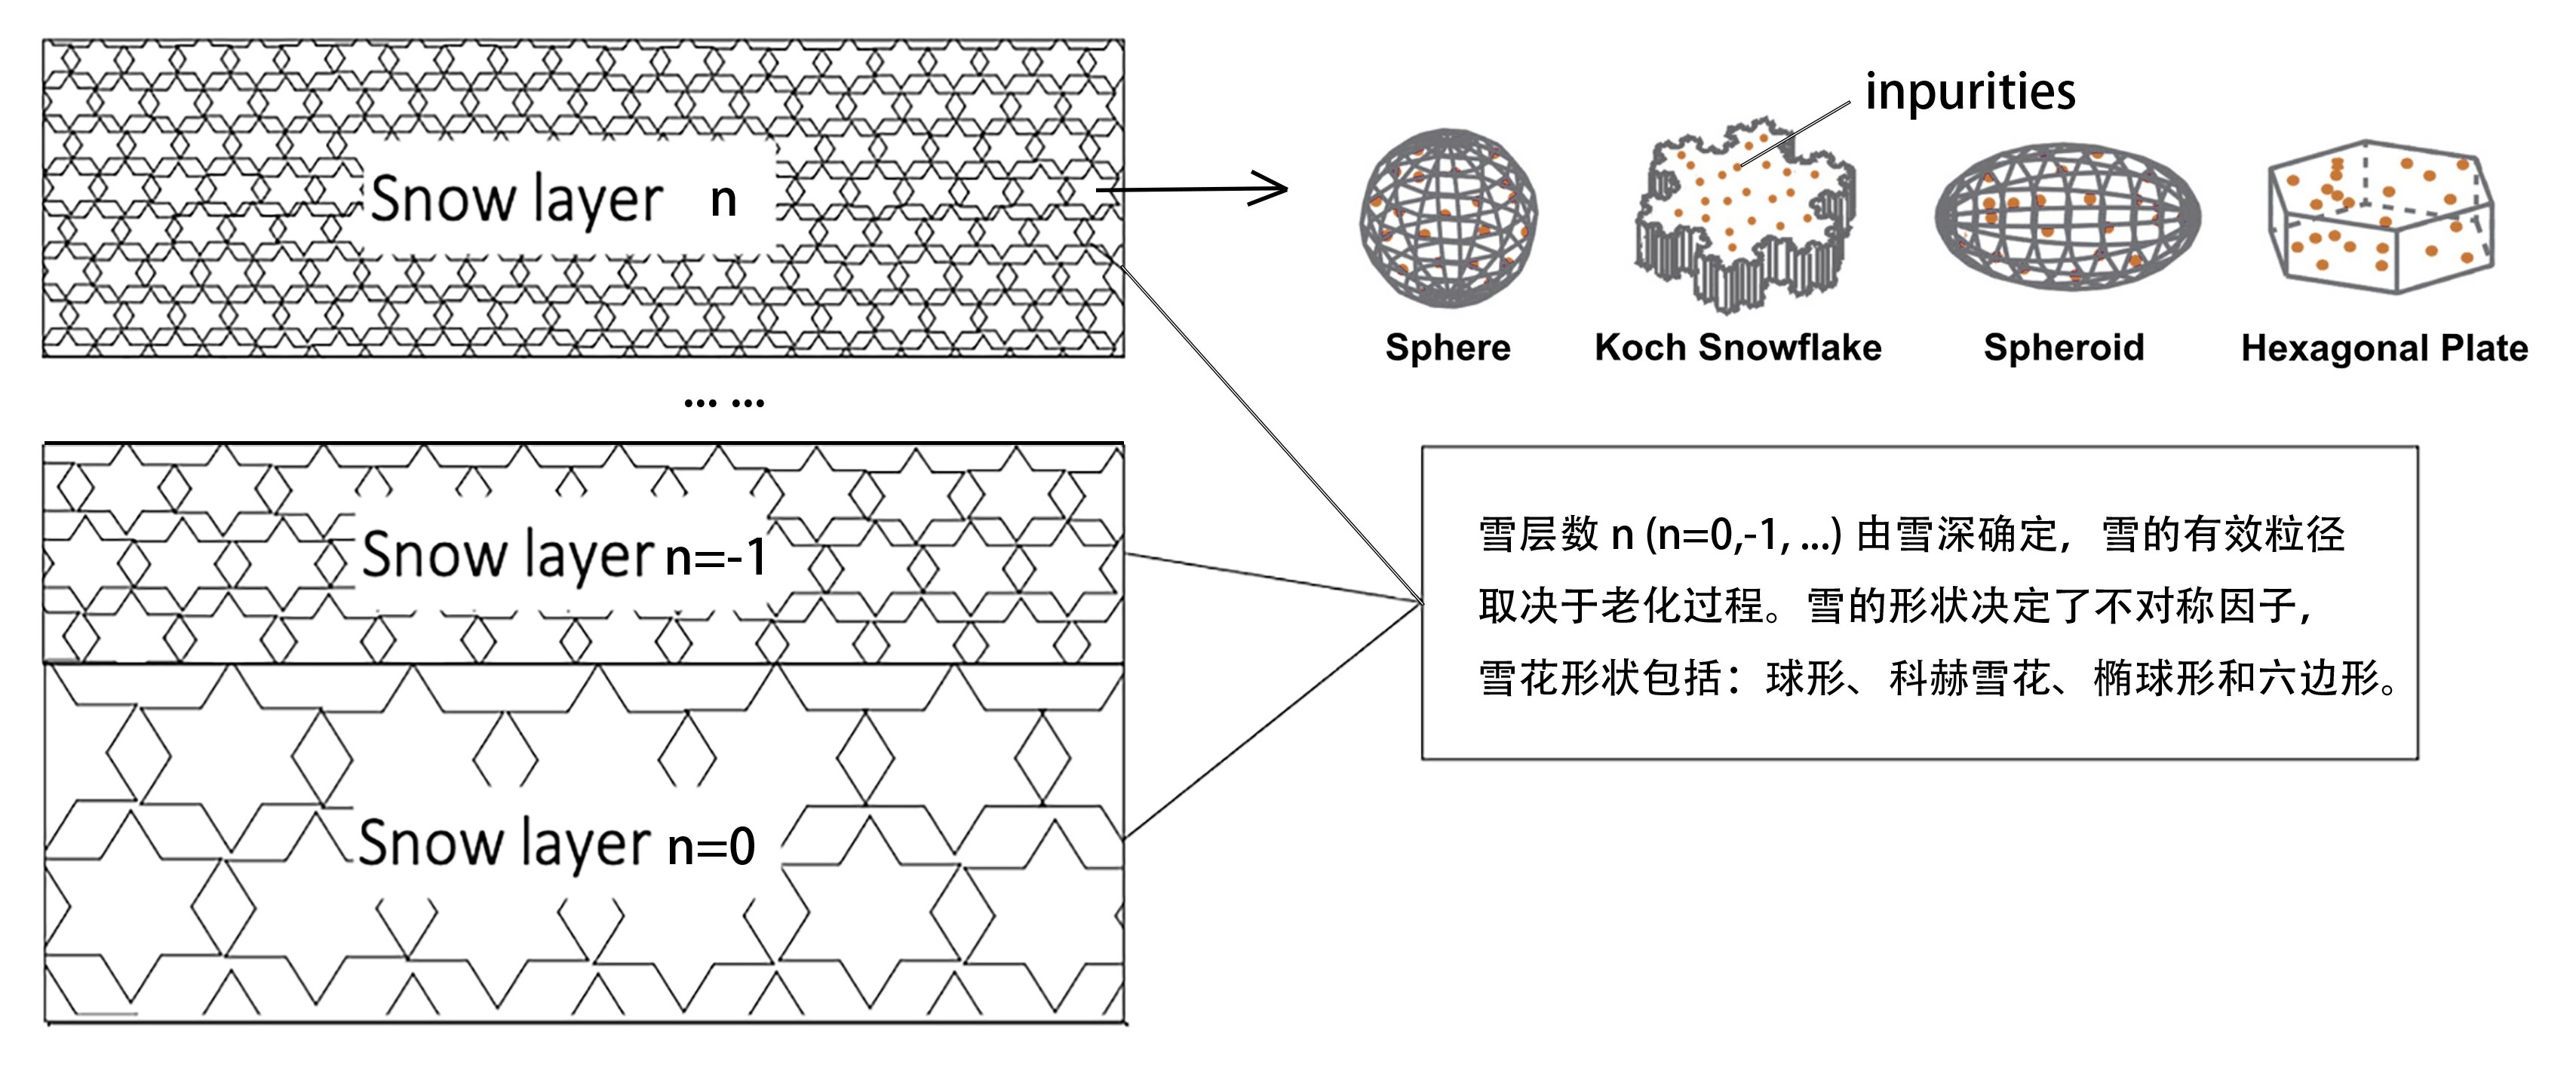
\includegraphics[width=0.9\columnwidth]{Figures/辐射过程及辐射通量计算/SNICAR积雪分层及雪花形状.jpg}
\caption[SNICAR积雪分层及雪花形状]{SNICAR积雪分层及雪花形状。图片基于\citet{he2017ImpactSnowGrain}和\citet{whicker2022SNICARADv4PhysicallyBased}修改}
\label{fig:SNICAR积雪分层及雪花形状}
\end{figure}
}

CoLM另一种积雪反照率及其对太阳辐射吸收的模拟,采用雪、冰和气溶胶辐射SNICAR (the Snow, Ice, and Aerosol Radiative) 模型 \citep{flanner2021SNICARADv3CommunityTool}。该模型采用多层积雪结构(图~\ref{fig:SNICAR积雪分层及雪花形状}),细致考虑每层光学属性,利用大气沉积气溶胶(黑炭、矿物粉尘、有机碳)、雪的有效粒径、太阳天顶角(\(\mu_{0}\))以及雪层所覆盖下垫面的反照率,采用\citet{toon1989RapidCalculationRadiative}的二流辐射传输方案来计算积雪反照率和垂直吸收廓线(图~\ref{fig:SNICAR模型流程图})。

{
\begin{figure}[htbp]
\centering
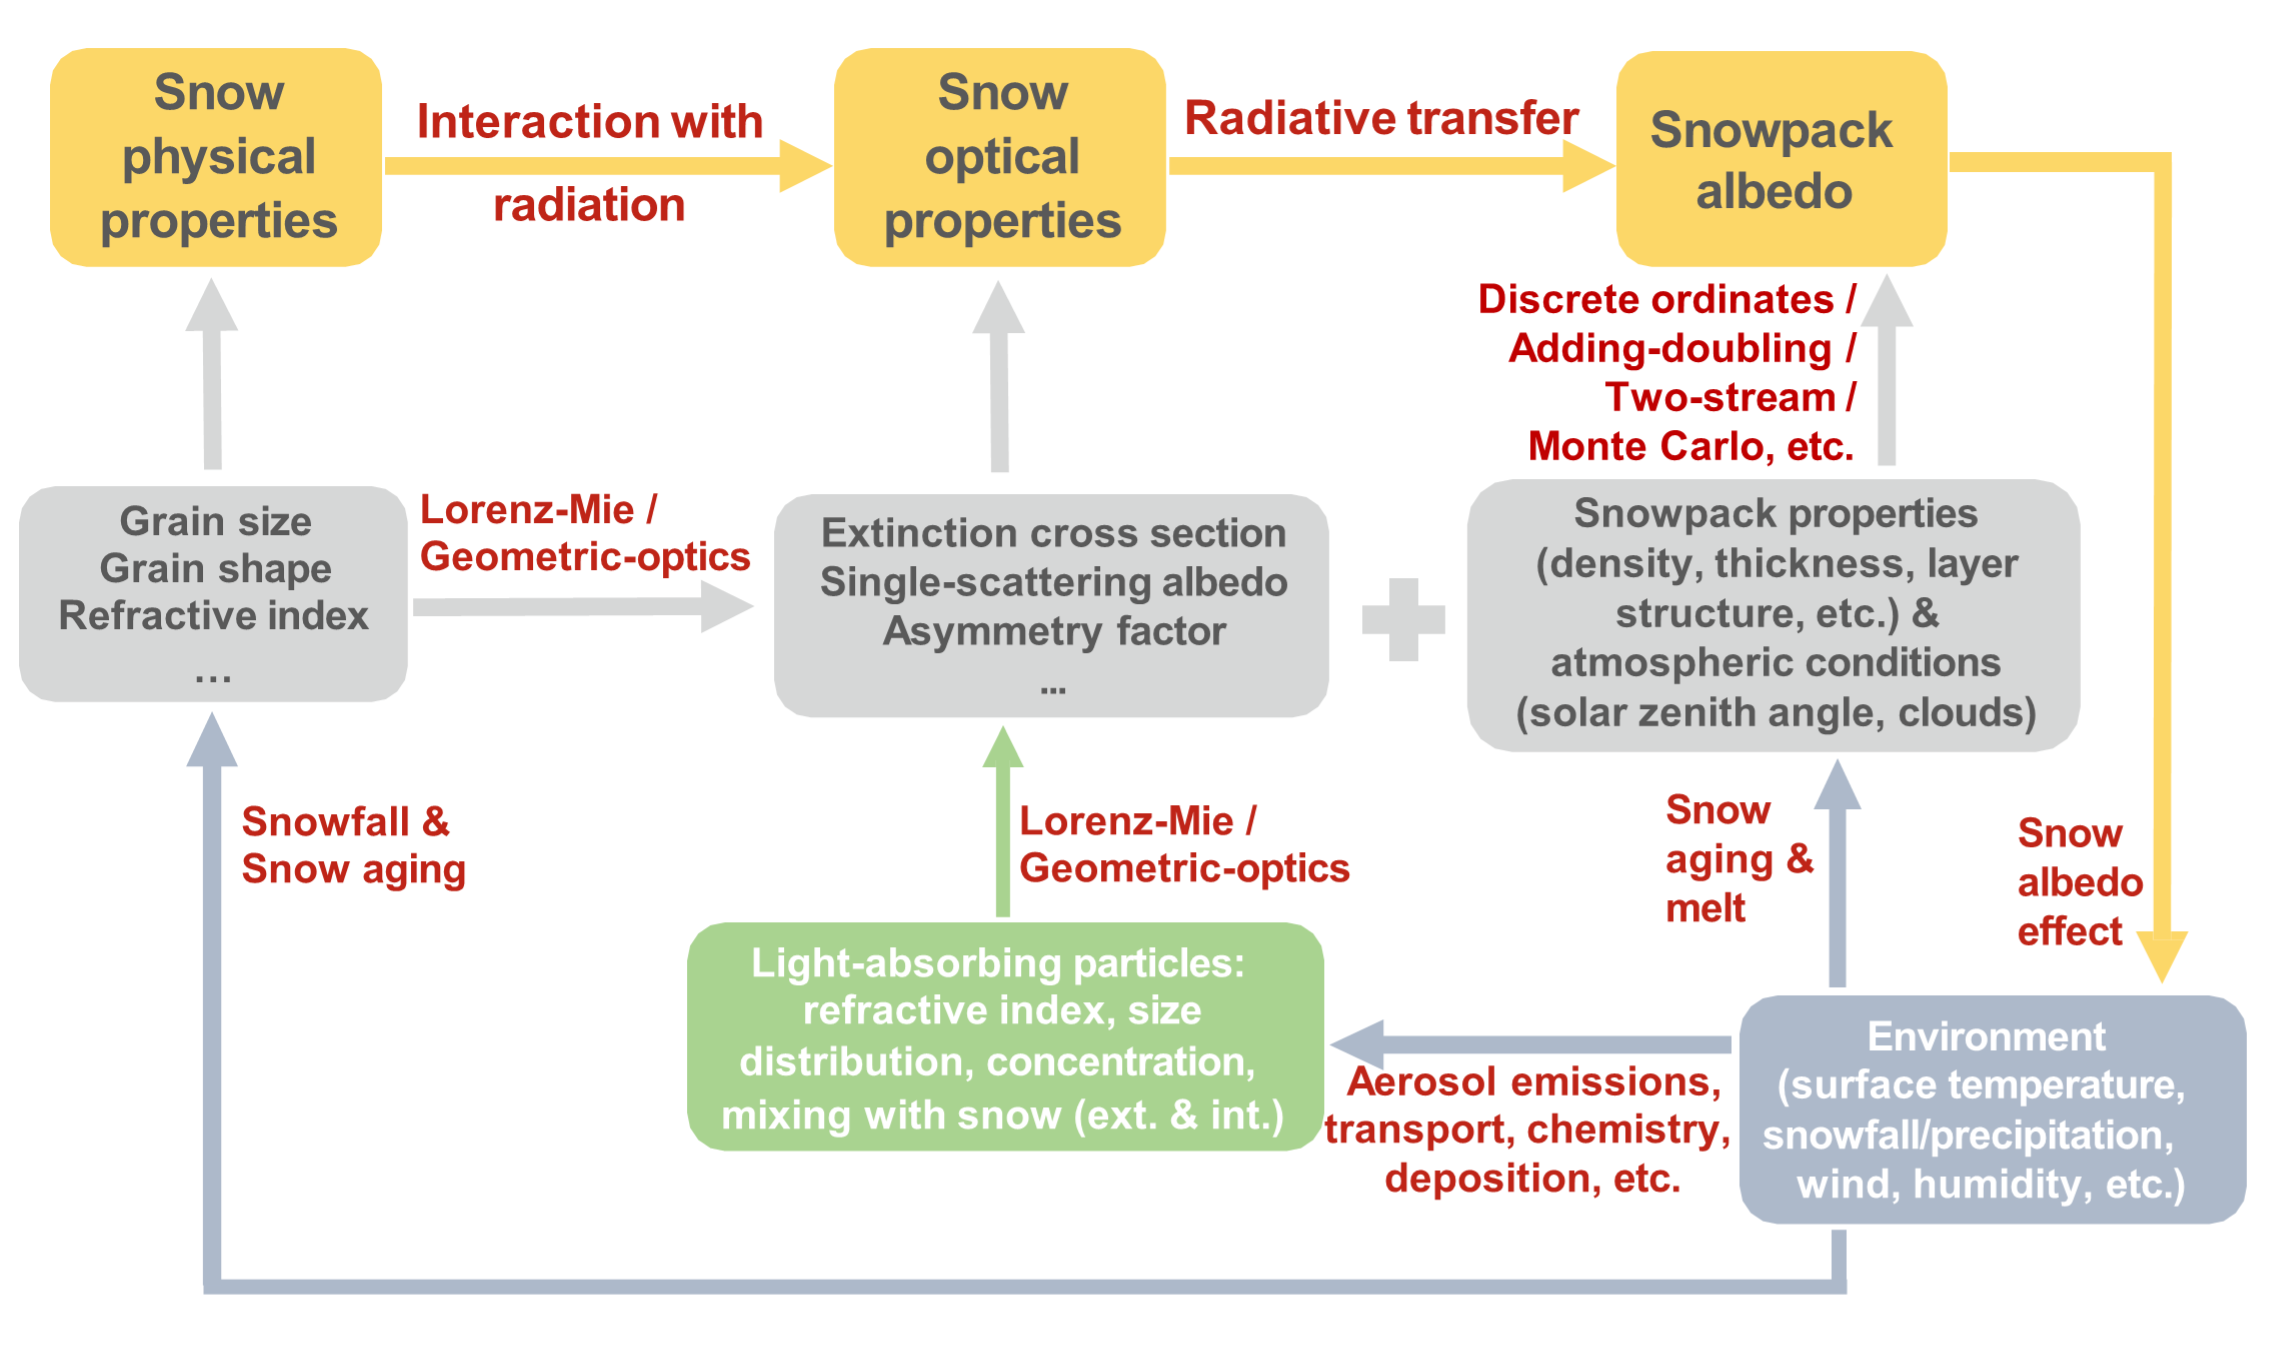
\includegraphics[width=1\columnwidth]{Figures/辐射过程及辐射通量计算/SNICAR模型计算流程图.png}
\caption{SNICAR积雪反照率计算流程图\citep{he2020SnowAlbedoRadiative}}
\label{fig:SNICAR模型流程图}
\end{figure}
}

二流近似方案(two-stream
solution)需要使用到每个雪层和光谱波段的以下光学属性:光学厚度($\tau$),
单次散射反照率($\omega$),
以及散射不对称性因子($g$)。SNICAR中,体散射光学属性是每种成分$k$的加权函数,针对每个雪层和光谱波段进行计算。

\begin{equation}
\tau = \sum_{1}^{k}\tau_{k}
\end{equation}
%
\begin{equation}
\omega = \frac{\sum_{1}^{k}\omega_{k}\tau_{k}}{\sum_{1}^{k}\tau_{k}}
\end{equation}
%
\begin{equation}
g = \frac{\sum_{1}^{k}{g_{k}\omega}_{k}\tau_{k}}{\sum_{1}^{k}\omega_{k}\tau_{k}}
\end{equation}

对于每种成分(冰粒、两种黑碳、两种有机碳、四种沙尘),$\tau$、$g$和质量消光截面$\psi$(\unit{m^2.kg^{-1}})使用米氏散射近似进行计算。每种成分的光学厚度取决于各自的质量消光截面和各层质量,从而可以得到:
\begin{equation}
\tau_{k} = \psi_{k}\omega_{k}
\end{equation}

\subsubsection{积雪的光学属性}
冰粒在五个波段的光学属性为离线获得,并存储在相应的检索表中。米氏散射属性先在较高的光谱分辨率下计算,再根据入射太阳通量\(I^{\downarrow}(\lambda)\)对五个波段进行加权。波长区间在$\lambda_{1}-\lambda_{2}$的质量消光截面(\(\overline{\psi}\))表达式为:

\begin{equation}
\overline{\psi} = \frac{\int_{\lambda_{2}}^{\lambda_{1}}{\psi(\lambda)I^{\downarrow}(\lambda)d\lambda\ }}{\int_{\lambda_{2}}^{\lambda_{1}}{I^{\downarrow}(\lambda)d\lambda\ }}
\end{equation}

对于半无限厚的雪盖,宽波段的单次散射反照率(\(\overline{\omega}\))由漫射反照率加权得到:
\begin{equation}
\overline{\omega} = \frac{\int_{\lambda_{2}}^{\lambda_{1}}{\omega(\lambda){I^{\downarrow}(\lambda)\alpha}_{sno}(\lambda)d\lambda\ }}{\int_{\lambda_{2}}^{\lambda_{1}}{I^{\downarrow}(\lambda)\alpha_{sno}(\lambda)d\lambda\ }}
\end{equation}

积雪反照率十分依赖于冰粒的单次散射反照率,包含额外的反照率权重可以提高五个波段反照率方案的准确性\citep{flanner2007PresentdayClimateForcing}。

积雪在五种波段的单次散射反照率、质量消光截面以及不对称参数由表~\ref{tab:积雪单次散射反照率} 给出,它们均基于米氏散射近似理论计算得到。不同大气沉积气溶胶的单次散射反照率、质量消光截面以及不对称参数取决于波段。而对于冰粒,其光学属性取决于入射辐射类型(直射或漫射辐射)、波段以及有效粒径,其中有效粒径考虑积雪的老化过程计算得到(见章节~\ref{积雪老化})。

积雪中的成分包括冰粒和沉积在雪中的吸光物质,它们直接决定了积雪的光学属性。SNICAR模型考虑了不同的雪花形状,分别为球形、椭球形、科赫雪花、六边形雪花\citep{he2017ImpactSnowGrain},再根据不同波段,从而确定了不对称因子(图~\ref{fig:SNICAR积雪分层及雪花形状})。

\begin{table}[htbp]
\centering
\caption{雪中杂质和冰粒的单次散射反照率$\omega$}
\label{tab:积雪单次散射反照率}
\begin{tabular}{llllll}
\toprule
种类 & 波段一 & 波段二 & 波段三 & 波段四 & 波段五 \\ \midrule
亲水黑碳 & 0.516 & 0.516 & 0.516 & 0.516 & 0.516 \\
疏水黑碳 & 0.288 & 0.288 & 0.288 & 0.288 & 0.288 \\
亲水有机碳 & 0.997 & 0.997 & 0.997 & 0.997 & 0.997 \\
疏水有机碳 & 0.963 & 0.963 & 0.963 & 0.963 & 0.963 \\
沙尘一 & 0.979 & 0.979 & 0.979 & 0.979 & 0.979 \\
沙尘二 & 0.944 & 0.944 & 0.944 & 0.944 & 0.944 \\
沙尘三 & 0.904 & 0.904 & 0.904 & 0.904 & 0.904 \\
沙尘四 & 0.850 & 0.850 & 0.850 & 0.850 & 0.850 \\
冰($r_{e}=30$ $\mu\rm{m}$) & 0.9999 & 0.9999 & 0.9999 & 0.9999 &
0.9999 \\
冰($r_{e}=1500$ $\mu\rm{m}$) & 0.9998 & 0.9998 & 0.9998 & 0.9998 &
0.9998 \\ \bottomrule
\end{tabular}
\end{table}

\begin{table}[htbp]
\centering
\caption{雪中杂质和冰粒的质量消光系数$\tau$}
\label{tab:积雪消光系数}
\begin{tabular}{llllll}
\toprule
种类 & 波段一 & 波段二 & 波段三 & 波段四 & 波段五 \\ \midrule
亲水黑碳 & 25369 & 25369 & 25369 & 25369 & 25369 \\
疏水黑碳 & 11398 & 11398 & 11398 & 11398 & 11398 \\
亲水有机碳 & 37774 & 37774 & 37774 & 37774 & 37774 \\
疏水有机碳 & 3289 & 3289 & 3289 & 3289 & 3289 \\
沙尘一 & 2687 & 2687 & 2687 & 2687 & 2687 \\
沙尘二 & 841 & 841 & 841 & 841 & 841 \\
沙尘三 & 388 & 388 & 388 & 388 & 388 \\
沙尘四 & 197 & 197 & 197 & 197 & 197 \\
冰($r_{e}=30$ $\mu\rm{m}$) & 55.7 & 55.7 & 55.7 & 55.7 & 55.7 \\
冰($r_{e}=1500$ $\mu\rm{m}$) & 1.09 & 1.09 & 1.09 & 1.09 & 1.09 \\ \bottomrule
\end{tabular}
\end{table}

\begin{table}[htbp]
\centering
\caption{雪中杂质和冰粒的不对称参数$g$}
\label{tab:积雪不对称参数}
\begin{tabular}{llllll}
\toprule
种类 & 波段一 & 波段二 & 波段三 & 波段四 & 波段五 \\ \midrule
亲水黑碳 & 0.52 & 0.52 & 0.52 & 0.52 & 0.52 \\
疏水黑碳 & 0.35 & 0.35 & 0.35 & 0.35 & 0.35 \\
亲水有机碳 & 0.77 & 0.77 & 0.77 & 0.77 & 0.77 \\
疏水有机碳 & 0.62 & 0.62 & 0.62 & 0.62 & 0.62 \\
沙尘一 & 0.69 & 0.69 & 0.69 & 0.69 & 0.69 \\
沙尘二 & 0.70 & 0.70 & 0.70 & 0.70 & 0.70 \\
沙尘三 & 0.79 & 0.79 & 0.79 & 0.79 & 0.79 \\
沙尘四 & 0.83 & 0.83 & 0.83 & 0.83 & 0.83 \\
冰($r_{e}=30$ $\mu\rm{m}$) & 0.88 & 0.88 & 0.88 & 0.88 & 0.88 \\
冰($r_{e}=1500$ $\mu\rm{m}$) & 0.89 & 0.89 & 0.89 & 0.89 & 0.89\\ \bottomrule
\end{tabular}
\end{table}

\subsubsection{积雪老化过程}\label{积雪老化}

雪的老化表现为冰粒有效粒径($r_e$)的变化。已有研究表明,使用由更复杂形状组成的冰介质表面积与体积比(或比表面积)的球体会在模拟半球通量中产生相对较小误差(例如~\citet{grenfell1999RepresentationNonsphericalIce})。有效半径是球形粒子集合的表面积加权平均半径,与比表面积(SSA)直接相关,表达式为$r_e=3/(\rho_{ice}\text{SSA})$,其中$\rho_{ice}$是冰的密度。$r_e$是一个简单实用的度量指标,将积雪微观物理状态与干雪辐射特性联系起来。

雪变湿的过程也会导致反照率快速变化。液态水的存在会导致周围的冰粒迅速变得粗糙(例如~\citet{brun1989InvestigationWetSnowMetamorphism}),液态水往往会重新冻结成较大的冰块,使积雪变暗。小液滴的存在本身不会地使积雪显著变暗,因为冰和水的折射率在整个太阳光谱中非常接近。然而,积水会大大减少每单位质量的折射事件的发生,从而使积雪变暗。目前还没有考虑到这种影响。

每个时间步长发生的有效晶粒度的净变化在每个雪层中可以概括为干雪变质作用($dr_{e,dry}$)、液态水导致的变质作用($dr_{e,wet}$)、液体水的再冻结和新降雪的加入引起的变化。每个雪层的质量被划分为上一个时间步长遗留下来的雪($f_{old}$)、新降雪($f_{new}$)和重新冻结的液态水($f_{rfz}$),使得雪的$r_e$在每个时间步长${t}$更新为:
\begin{equation}
r_{e}(t) = \lbrack r_{e}(t - 1) + {dr}_{e,dry} + {dr}_{e,wet}\rbrack f_{old} + r_{e,0}f_{new} + r_{e,rfz}f_{rfz}
\end{equation}

新降雪($r_{e,0}$)的有效粒径仅基于其与温度的简单线性关系。低于$-30$摄氏度时,有效粒径的最小值被强制取为54.5 \unit{\mu{m}}(对应60 \unit{m^{2}.kg^{-1}});大于0摄氏度时,有效粒径的最大值被强制取为204.5 \unit{\mu{m}}。有效粒径在$-30$和0摄氏度之间为线性变化。重新冻结的液态水($r_{e,rfz}$)的有效粒径设置为1000 \unit{\mu{m}}。

干雪的老化基于~\citet{flanner2006LinkingSnowpackMicrophysics}描述的微观物理模型。该模型模拟了不同尺寸和颗粒间距的冰晶集合之间的扩散水蒸汽通量。根据雪温度、温度梯度、密度和初始颗粒大小分布的任何组合,预测比表面积和有效半径。高温、较大的温度梯度以及较小的雪密度最有利于加速雪的老化,而在低温下,无论温度梯度和密度如何,雪的老化都会缓慢进行。由于该模型目前计算成本太高,无法纳入气候模型,我们将参数曲线拟合为大范围雪况下的输出模型,并将这些参数应用于模型中。参数方程的函数形式为:
\begin{equation}
\frac{{dr}_{e,dry}}{dt} = \left( \frac{{dr}_{e}}{dt} \right)_{0}\left( \frac{\eta}{r_{e} - r_{e,0} + \eta} \right)^{1/\kappa}
\end{equation}

参数$\left( \frac{{dr}_{e}}{dt} \right)_{0}$,$\eta$和$\kappa$以交互方式从具有与积雪温度、温度梯度和密度相对应的查找表中检索。该查找表所涵盖的温度范围为223--273 K、温度梯度范围为0--300 \unit{K.m^{-1}},密度范围为50--400 \unit{kg.m^{-3}}。温度梯度$\left( \frac{dT}{dz} \right)_{n}$由雪层温度($T_n$)雪层厚度($dz_n$)和雪覆盖度($f_{sno}$)计算得到:
%
\begin{equation}
\left( \frac{dT}{dz} \right)_{n} = \frac{1}{f_{sno}\cdot {dz}_{n}}\left| \frac{T_{n - 1}{dz}_{n} + T_{n}{dz}_{n - 1}}{{dz}_{n} + {dz}_{n - 1}} - \frac{T_{n + 1}{dz}_{n} + T_{n}{dz}_{n + 1}}{{dz}_{n} + {dz}_{n + 1}} \right|
\end{equation}
%
对于底部雪层($n=0$),$T_{n+1}$为表层土壤的温度;对于表层雪,假设$T_{n-1}=T_n$。

液态水对加强的变质作用的贡献基于~\citet{brun1989InvestigationWetSnowMetamorphism}中的参数方程,不同液态水含量下的粒径增长率$\frac{{dr}_{e}}{dt}$取决于液态水质量分数$f_{liq}$:
%
\begin{equation}
\frac{{dr}_{e}}{dt} = \frac{10^{18}C_{1}f_{liq}^{3}}{4\pi r_{e}^{2}}
\end{equation}
%
其中$C_{1}$为$4.22×10^{-13}$,$f_{liq}=w_{liq}/(w_{liq}+w_{ice})$,$w_{liq}$和$w_{ice}$分别表示雪层中液态水和固态水的含量(\unit {kg.m^{-2}})。 

在雪质量大于零但尚未定义雪层的情况下,$r_e$设置为$r_{e,0}$,当雪层被合并或分割时,$r_e$根据其他状态变量的计算,计算为两层的质量加权平均值。计算得到的$r_e$的范围限制在30--1500 \unit{\mu{m}}之间。

\subsubsection{SNICAR模型二流近似求解}

对于多层积雪辐射传输二流近似求解,SNICAR模型提供了两种可供选择的方案:SNICAR\_RT \citep{dang2019IntercomparisonImprovementTwostream}与SNICAR\_AD\_RT方案\citep{flanner2021SNICARADv3CommunityTool}。

1、SNICAR\_RT

SNICAR\_RT在二流近似中使用了三对角矩阵方案(tri-diagonal
solution, \citet{toon1989RapidCalculationRadiative}),在每层界面计算向上和向下的辐射通量,从中可以推导出净辐射吸收、每层吸收和表面反照率,三对角矩阵方案包含了二流近似方案的中间项。SNICAR\_RT对可见光波段使用的是Eddington近似\citep{wiscombe1980ModelSpectralAlbedo},对近红外波段使用Hemispheric mean \citep{toon1989RapidCalculationRadiative},这样选择是因为Eddington近似方案适用于高强度散射的介质。

二流近似从水平均一介质辐射传输的一般方程所导出:
%
\begin{equation}
\mu\frac{\partial {I}}{\partial\tau}(\tau,\mu,\phi){= I(\tau,}\mu,\Phi) - \frac{\omega}{{4}{\pi}}\int_{{0}}^{{2}\pi}{\int_{- 1}^{1}{P\left( \mu,\mu^{'},\Phi,\Phi^{'} \right)}}I\left( \tau,\mu^{'},\Phi^{'} \right){d}\mu^{'}d\Phi^{'}{- S}\left( \tau,\mu,\Phi \right)
\end{equation}
%
其中\(\Phi\)是方位角,\(\mu\)是天顶角的余弦,\(\omega\)是单次散射反照率。等式右侧的三项分别为:光学厚度为\(\tau\)时的强度、多次散射引起的内源项和外部源函数$S$。对于太阳波长的纯外部光源,$S$为:
%
\begin{equation}
S = \frac{\omega}{4}F_{s}P\left( \mu,{- \mu}_{0},\Phi,\Phi_{0} \right)\exp\left( -\frac{\mathbf{\tau}}{\mu_{0}} \right)
\end{equation}

\citet{meador1980TwostreamApproximationsRadiative}指出,二流近似的表示式可以写成以下形式:
\begin{equation}
\frac{dF_{n}^{+}(\tau)}{d\tau_{n}} = \gamma_{1n}F_{n}^{+} - \gamma_{2n}F_{n}^{-} - S_{n}^{+}
\end{equation}
\begin{equation}
\frac{dF_{n}^{-}(\tau)}{d\tau_{n}} = \gamma_{2n}F_{n}^{+} - \gamma_{1n}F_{n}^{-} + S_{n}^{+}
\end{equation}
其中,\(\gamma_{1}\)和\(\gamma_{2}\)是取决于二流近似方程的特定形式的系数。我们通过用$n$(层数)标记通量来得到多层的解决方案。

\begin{table}[htbp]
\centering
\caption{SNICAR中包含的二流近似系数取值}
\label{tab:SNICAR二流近似系数}
\begin{tabular}{llll}
\toprule
方法 & $\gamma_{1}$ & $\gamma_{2}$ & $\gamma_{3}$ \\ \midrule
Eddington &
\(\frac{\mathbf{1}}{\mathbf{4}}\left\lbrack \mathbf{7 - (4 + 3}g^{*})\omega^{*} \right\rbrack\)
&
\(- \frac{\mathbf{1}}{\mathbf{4}}\left\lbrack \mathbf{1 - (4 - 3}g^{*})\omega^{*} \right\rbrack\)
& \(\frac{\mathbf{1}}{\mathbf{4}}\mathbf{(2 - 3}g^{*}\mu_{0})\) \\
Hemispheric mean & \(\mathbf{2 - (1 +}g^{*})\omega^{*}\) &
\(\mathbf{(1 -}g^{*})\omega^{*}\) &
\(\frac{\mathbf{1}}{\mathbf{2}}\left\lbrack \mathbf{1 -}\sqrt{\mathbf{3}}g^{*}\mu_{0} \right\rbrack\) \\
Quadrature &
\(\frac{\sqrt{\mathbf{3}}}{\mathbf{2}}\left\lbrack \mathbf{2 - (1 +}g^{*})\omega^{*} \right\rbrack\)
& \(\frac{\sqrt{\mathbf{3}}}{\mathbf{2}}\mathbf{(1 -}g^{*})\omega^{*}\)
&
\(\frac{\mathbf{1}}{\mathbf{2}}\left\lbrack \mathbf{1 -}\sqrt{\mathbf{3}}g^{*}\mu_{0} \right\rbrack\) \\ \bottomrule
\end{tabular}
\end{table}

对于直射入射太阳辐射:
\begin{equation}
S^{+} = \gamma_{3}\pi F_{s}\omega_{0}\exp\left( - \left( \tau_{c} + \tau \right)/\mu_{0} \right)
\end{equation}
\begin{equation}
S^{-} = \gamma_{4}\pi F_{s}\omega_{0}\exp\left( - \left( \tau_{c} + \tau \right)/\mu_{0} \right)
\end{equation}
\begin{equation}
\frac{dF^{\uparrow}(\tau)}{d\tau} = \gamma_{1}F^{\uparrow}(\tau) - \gamma_{2}F^{\downarrow}(\tau) - \gamma_{3}\widetilde{\omega}F_{\odot}\exp( - \frac{\tau}{\mu_{0}})
\end{equation}
\begin{equation}
\frac{dF^{\downarrow}(\tau)}{d\tau} = \gamma_{1}F^{\uparrow}(\tau) - \gamma_{1}F^{\downarrow}(\tau) + (1 - \gamma_{3})\widetilde{\omega}F_{\odot}\exp( - \frac{\tau}{\mu_{0}})
\end{equation}
其中\(\pi F_{s}\)是入射太阳通量,\(\mu_{0}\)是太阳辐射的入射方向,以上两式可以得到二流近似的通解。求解系数的关键步骤是计算相函数。然而,简单的近似方法,比如Eddington近似,通常难以处理高度非对称的相函数(例如冰晶相函数)。一种常见的解决方案是通过使用$\delta$函数来近似相函数的强前向散射峰,并对相函数进行二流展开,从而得到广泛使用的``$\delta$函数调整"方法\citep{joseph1976DeltaEddingtonApproximationRadiative}。$\delta$函数调整能够提高在相函数高度非对称情况下的不同二流近似的准确性,表达式如下:
\begin{equation}
\tau^{*} = (1 - \omega g^{2})\tau
\end{equation}
\begin{equation}
\omega^{*} = \frac{(1 - g^{2})\omega}{1 - \omega g^{2}}
\end{equation}
\begin{equation}
g^{*} = \frac{g}{1 + g}
\end{equation}

\citet{meador1980TwostreamApproximationsRadiative}的研究指出,在第$n$层、光学厚度为\(\tau\)时,向上和向下的辐射通量可以表示为:
\begin{equation}
F_{n}^{+} = k_{1n}\exp\left( \Lambda_{n}\mathbf{\tau} \right) + \Gamma_{n}k_{2n}\exp\left( {- \Lambda}_{n}\mathbf{\tau} \right) + C_{n}^{+}(\mathbf{\tau)}
\end{equation}
\begin{equation}
F_{n}^{-} = \Gamma_{n}k_{1n}\exp\left( \Lambda_{n}\mathbf{\tau} \right) + k_{2n}\exp\left( {- \Lambda}_{n}\mathbf{\tau} \right) + C_{n}^{-}(\mathbf{\tau)}
\end{equation}
%
\(\Lambda_{n}\)、\(\Gamma_{n}\)和\(C_{n}\)分别为由二流方法、入射太阳通量和太阳高度角确定的已知系数,\(k_{1n}\)和\(k_{2n}\)为由边界条件确定的未知系数。
\begin{equation}
\Lambda = \sqrt{\gamma_{1} - \gamma_{2}}
\end{equation}
\begin{equation}
\Gamma = \frac{\gamma_{2}}{\gamma_{1} + \Lambda} = \frac{\gamma_{1} - \Lambda}{\gamma_{2}}
\end{equation}

对于太阳直射辐射,我们有:
\begin{equation}
C^{+}(\mathbf{\tau}) = \frac{\omega F_{0}\left\lbrack \left( \gamma_{1} - 1/\mu_{0} \right)/\gamma_{3} + \gamma_{2}\gamma_{4} \right\rbrack e^{- \left( \mathbf{\tau}_{c} + \mathbf{\tau} \right)/\mu_{0}}}{\Lambda^{2} - 1/\mu_{0}^{2}}
\end{equation}
\begin{equation}
C^{-}(\mathbf{\tau}) = \frac{\omega F_{0}\left\lbrack \left( \gamma_{1} + 1/\mu_{0} \right)/\gamma_{4} + \gamma_{2}\gamma_{3} \right\rbrack e^{- \left( \mathbf{\tau}_{c} + \mathbf{\tau} \right)/\mu_{0}}}{\Lambda^{2} - 1/\mu_{0}^{2}}
\end{equation}

当没有直射入射辐射时,\(C^{+}(\mathbf{\tau})\)和\(C^{-}(\mathbf{\tau})\)为零。

2、SNICAR\_AD\_RT

SNICAR\_AD\_RT使用了Delta-Eddington
Adding-Doubling方案。在$\delta$函数调整后,再应用二流近似(Eddington),将得到的$\tau^*$,$\omega^*$和$g^*$计算得到如下的各个中间量:
\begin{equation}
\Gamma = \sqrt{3(1 - \omega^{*})(1 - \omega^{*}g^{*})}
\end{equation}
\begin{equation}
u = \frac{3}{2}\left( \frac{1 - \omega^{*}g^{*}}{\Gamma} \right)
\end{equation}
\begin{equation}
N = {(u + 1)}^{2}e^{\Gamma\tau^{*}} - {(u - 1)}^{2}e^{- \Gamma\tau^{*}}
\end{equation}
\begin{equation}
\eta = \frac{3}{4}\omega^{*}\mu_{0}\left( \frac{1 + g^{*}(1 - \omega^{*})}{1 - \Gamma^{2}\mu_{0}^{2}} \right)
\end{equation}
\begin{equation}
\Upsilon = \frac{1}{2}\omega^{*}\left( \frac{1 + {3g}^{*}(1 - \omega^{*})\mu_{0}^{2}}{1 - \Gamma^{2}\mu_{0}^{2}} \right)
\end{equation}

每层对直接辐射的反射率($R$)和透射率($T$)分别可以表示为:
\begin{equation}
R\left( \mu_{0} \right) = \frac{1}{N}(\eta + \Upsilon)\left( u^{2} - 1 \right)\left( e^{\Gamma\tau^{*}} - e^{- \Gamma\tau^{*}} \right) + (\eta - \Upsilon)\left\lbrack \frac{4u}{N}e^{\frac{- \tau^{*}}{\mu_{0}}} - 1 \right\rbrack
\end{equation}
\begin{equation}
T\left( \mu_{0} \right) = (\eta + \Upsilon)\frac{4u}{N} + \left\lbrack \frac{1}{N}(\eta - \Upsilon)\left( u^{2} - 1 \right)\left( e^{\Gamma\tau^{*}} - e^{- \Gamma\tau^{*}} \right) - \eta - \Upsilon + 1 \right\rbrack e^{\frac{- \tau^{*}}{\mu_{0}}}
\end{equation}

对于漫射辐射的反射和透射率(\(\overline{R}\)和\(\overline{T}\))是根据~\citet{wiscombe1980ModelSpectralAlbedo}的假设,即在各向同性入射情况下,通过对直接辐射的反射率进行积分计算得到的。
%
\begin{equation}
\overline{R}\left( \mu_{0} \right) = 2\int_{0}^{+ 1}{\mu R(\mu)d\mu}
\end{equation}
\begin{equation}
\overline{T}\left( \mu_{0} \right) = 2\int_{0}^{+ 1}{\mu T(\mu)d\mu}
\end{equation}
%
对于反射率($R$)和透射率($T$)的数值求解是由8个高斯角积分得到。

在考虑层与层多次散射时,假设一旦辐射被散射,它就是漫射和各向同性的。对于位于上层的任意层1(具有辐射特性\(R_{1}\left( \mu_{0} \right)\)、\(T_{1}\left( \mu_{0} \right)\)、\({\overline{R}}_{1}\)、\({\overline{T}}_{1}\)),其下方是层2(具有辐射特性\(R_{2}\left( \mu_{0} \right)\)、\(T_{2}\left( \mu_{0} \right)\)、\({\overline{R}}_{2}\)、\({\overline{T}}_{2}\)),从上方入射的直射和漫射辐射的反射率、透射率计算为\citep{briegleb2007delta}:
\begin{equation}
R_{12}\left( \mu_{0} \right) = R_{1}\left( \mu_{0} \right) + \frac{\left\lbrack \left( T_{1}\left( \mu_{0} \right) - e^{- \tau^{*}/\mu_{0}} \right){\overline{R}}_{2} + e^{- \tau^{*}/\mu_{0}}R_{2}\left( \mu_{0} \right) \right\rbrack{\overline{T}}_{1}}{1 - {\overline{R}}_{1}{\overline{R}}_{2}}
\end{equation}
\begin{equation}
T_{12}\left( \mu_{0} \right) = {e^{- \tau^{*}/\mu_{0}}T}_{2}\left( \mu_{0} \right) + \frac{\left\lbrack \left( T_{1}\left( \mu_{0} \right) - e^{- \tau^{*}/\mu_{0}} \right) + e^{- \tau^{*}/\mu_{0}}R_{2}\left( \mu_{0} \right){\overline{R}}_{1} \right\rbrack{\overline{T}}_{2}}{1 - {\overline{R}}_{1}{\overline{R}}_{2}}
\end{equation}
\begin{equation}
{\overline{R}}_{12} = {\overline{R}}_{1} + \frac{{\overline{T}}_{1}{\overline{R}}_{2}{\overline{T}}_{1}}{1 - {\overline{R}}_{1}{\overline{R}}_{2}}
\end{equation}
\begin{equation}
{\overline{T}}_{12} = \frac{{\overline{T}}_{1}{\overline{T}}_{2}}{1 - {\overline{R}}_{1}{\overline{R}}_{2}}
\end{equation}

从下方照射时的透射率是相同的,而反射率假定为从上方漫射照射时的向上反射率\({\overline{R}}_{12}\),但下标的层序号相反。累积的雪层界面光学属性,对于向下传播和向上传播的辐射,是通过循环求解的,从雪层的顶部向下积分,然后从底部向上积分。在从顶部向下计算辐射传输时,如果所在波段总透射率(在顶部归一化为1.0)小于0.001,则终止\(R\left( x_{0} \right)\)、\(T\left( x_{0} \right)\)、\(R\)、\(T\)的计算。对于每个界面,都有以下变量:

``$\tau^{*}$''为雪层顶部到某一雪层交界面经调整的光学厚度。

``$R_{up}\left( \mu_{0} \right)$''为某一雪层交界面以下所有雪层对来自上方的向下直接辐射的反射率。

``$\overline{R}_{up}$''为某一雪层交界面以下所有雪层对来自上方的向下漫射辐射的反射率。

``$\overline{R}_{dn}$''为某一雪层交界面以上的所有雪层对来自下方的向上漫射辐射的反射率。

``$T_{dn}\left( \mu_{0} \right)$''为直射辐射从雪层顶部到某一雪层交界面的总透射率。

``$\overline{T}_{dn}$''为漫射辐射从雪层顶部到某一雪层交界面的总透射率。

基于以上变量,每个雪层交界面上的向下(\(F_{dir}^{\downarrow}\))和向上(\(F_{dir}^{\uparrow}\))辐射通量标准化为雪层顶部的单位直接入射通量,分别表示为:
\begin{equation}
F_{dir}^{\downarrow} = e^{- \tau^{*}/\mu_{0}} + \frac{\left( T_{dn}\left( \mu_{0} \right) - e^{- \tau^{*}/\mu_{0}} \right) + e^{- \tau^{*}/\mu_{0}}R_{up}\left( \mu_{0} \right){\overline{R}}_{dn}}{1 - {\overline{R}}_{dn}{\overline{R}}_{up}}
\end{equation}
\begin{equation}
F_{dir}^{\uparrow} = \frac{e^{- \tau^{*}/\mu_{0}}R_{up}\left( \mu_{0} \right) + \left( T_{dn}\left( \mu_{0} \right) - e^{- \tau^{*}/\mu_{0}} \right) + {\overline{R}}_{up}}{1 - {\overline{R}}_{dn}{\overline{R}}_{up}}
\end{equation}

每个雪层交界面上的向下(\(F_{dif}^{\downarrow}\))和向上(\(F_{dif}^{\uparrow}\))通量标准化为模型顶部的单位漫射入射通量,分别表示为:
\begin{equation}
F_{dif}^{\downarrow} = \frac{{\overline{T}}_{dn}}{1 - {\overline{R}}_{dn}{\overline{R}}_{up}}
\end{equation}
\begin{equation}
F_{dif}^{\uparrow} = \frac{{\overline{T}}_{dn}{\overline{R}}_{up}}{1 - {\overline{R}}_{dn}{\overline{R}}_{up}}
\end{equation}

最后,反照率\(\alpha\)由顶层界面的通量得到:
\begin{equation}
\alpha = \frac{F_{dir}^{\uparrow}(top) + F_{dif}^{\uparrow}(top)}{F_{dir}^{\downarrow}(top) + F_{dif}^{\downarrow}(top)}
\end{equation}

太阳辐射通量根据五个光谱波段来计算,如下表所示。由于雪的反照率在整个太阳光谱中变化较大,因此采用四个波段来更准确地表示雪在近红外(NIR,0.7--5.0 $\mu \rm{m}$)波段的特性,而对于可见光谱只采用一个波段。根据表中列出的权重划分向下NIR辐射通量,这些权重通过中纬度冬季典型大气的离线光谱辐射传输计算得到\citep{briegleb2007delta}。

\begin{table}[htbp]
\centering
\caption{分波段太阳辐射权重系数}
\label{tab:太阳辐射权重系数}
\begin{tabular}{lll}
\toprule
光谱波段 & 直接太阳辐射权重 & 漫射太阳辐射权重 \\ \midrule
波段1:0.3-0.7 $\mu \rm{m}$(可见光) & 1.0 & 1.0 \\
波段2:0.7-1.0 $\mu \rm{m}$(近红外) & 0.494 & 0.586 \\
波段3:1.0-1.2 $\mu \rm{m}$(近红外) & 0.181 & 0.202 \\
波段4:1.2-1.5 $\mu \rm{m}$(近红外) & 0.121 & 0.109 \\
波段5:1.5-5.0 $\mu \rm{m}$(近红外) & 0.204 & 0.103 \\ \bottomrule
\end{tabular}
\end{table}

\section{海洋反照率}\label{海洋反照率}
\begin{mymdframed}{代码}
对应代码为\texttt{MOD\_Albedo.F90}文件中\texttt{albocean()}函数。
\end{mymdframed}

对于有冰雪覆盖的海洋,当\(\mu < 0.5\)时,积雪区域反照率计算为:
%
\begin{equation}
\alpha_{sno,vis,dir} = \min\left( 0.98,\alpha_{sno,vis,dif} + 0.5\frac{1 - \alpha_{sno,vis,dif}}{\frac{3}{1 + 4\mu} - 1} \right)
\end{equation}
%
\begin{equation}
\alpha_{sno,nir,dir} = \min\left( 0.98,\alpha_{sno,nir,dif} + 0.5\frac{1 - \alpha_{sno,nir,dif}}{\frac{3}{1 + 4\mu} - 1} \right)
\end{equation}
%
其中\(\alpha_{sno,vis,dif} = \alpha_{newsno,vis} = 0.95\),\(\alpha_{sno,nir,dif} = \alpha_{newsno,nir} = 0.7\)。当\(\mu \geqslant 0.5\)时,相应值计算为:
%
\begin{equation}
\alpha_{sno,vis,dir} = \alpha_{newsno,vis}
\end{equation}
%
\begin{equation}
\alpha_{sno,nir,dir} = \alpha_{newsno,nir}
\end{equation}
%
积雪厚度计算为:
%
\begin{equation}
z_{sno} = \frac{20W_{sno}}{1000}
\end{equation}
%
其中\(W_{sno}\)为雪水当量(mm)。海面积雪覆盖度计算为:
\begin{equation}
f_{sno} = \frac{z_{sno}}{0.25 + z_{sno}}
\end{equation}
考虑积雪覆盖的海洋总体反照率计算为:
\begin{equation}
\alpha_{sea,vis,dir} = \alpha_{ice,vis}\left( 1 - f_{sno} \right) + \alpha_{sno,vis,dir}f_{sno}
\end{equation}
%
\begin{equation}
\alpha_{sea,nir,dir} = \alpha_{ice,nir}\left( 1 - f_{sno} \right) + \alpha_{sno,nir,dir}f_{sno}
\end{equation}
%
\begin{equation}
\alpha_{sea,vis,dif} = \alpha_{ice,vis}\left( 1 - f_{sno} \right) + \alpha_{sno,vis,dif}f_{sno}
\end{equation}
%
\begin{equation}
\alpha_{sea,nir,dif} = \alpha_{ice,nir}\left( 1 - f_{sno} \right) + \alpha_{sno,nir,dif}f_{sno}
\end{equation}
其中\(\alpha_{ice,vis} = 0.7\),\(\alpha_{ice,nir} = 0.5\)。

对于无冰雪覆盖海洋,假设反照率与波段和海表面风速等其他物理量无关,采用太阳高度角计算直射入射反照率,漫射反射率则设为常数,公式表达为:
\begin{equation}
\alpha_{sea,vis,dir}=\alpha_{sea,nir,dir} = \frac{0.026}{\mu^{1.7}+0.065}+0.15(\mu-0.1)(\mu-0.5)(\mu-1)
\end{equation}
%
\begin{equation}
\alpha_{sea,vis,dif}=\alpha_{sea,nir,dif} = 0.06
\end{equation}

\section{植被反照率---二流近似模型}\label{植被反照率二流近似模型}
\begin{mymdframed}{代码}
对应代码为\texttt{MOD\_Albedo.F90}文件中\texttt{twostream()}函数。
\end{mymdframed}

{
\begin{figure}[htbp]
\centering
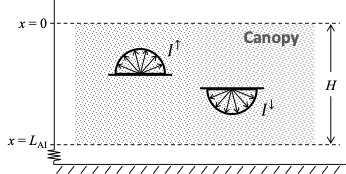
\includegraphics[width=0.7\columnwidth]{Figures/辐射过程及辐射通量计算/二流近似模型示意图.png}
\caption{二流近似植被辐射传输模型示意图}
\label{fig:二流近似模型示意图}
\end{figure}
}
植被反照率采用二流近似方法(two-stream approximation,\citet{dickinson1983land,sellers1985canopy}) 进行求解。在此基础上,利用双大叶模型 (two-big-leaf model) \citep{dai2004two} 对阴阳叶分别计算辐射吸收量。二流近似方法是把植被冠层内的辐射场看成是上下两个辐射流组成(图~\ref{fig:二流近似模型示意图}),这样可以把描述辐射传输的微分方程简化为两个联立的常微分方程组:
\begin{equation}\label{di_dx1}
-\bar{\mu} \frac{d I^{\uparrow}}{d x}+\left[1-(1-\beta) \omega\right] I^{\uparrow}-\omega \beta I^{\downarrow}=\omega \bar{\mu} K \beta_{0} \exp (-K x)
\end{equation}
\begin{equation}\label{di_dx2}
\bar{\mu} \frac{d I^{\downarrow}}{d x}+\left[1-(1-\beta) \omega\right] I^{\downarrow}-\omega \beta I^{\uparrow}=\omega \bar{\mu} K\left(1-\beta_{0}\right) \exp (-K x)
\end{equation}
其中$I^{\uparrow}$, $I^{\downarrow}$表示向上和向下的漫射通量,为相对于总入射辐射通量(直射或漫射)的归一化值。$\mu$为太阳天顶角余弦,$\bar{\mu}$为漫射辐射在单位叶面积上的光学厚度倒数平均值。$\beta$、$\beta_{0}$为漫射辐射和直射辐射向上散射(upscatter)系数,$\omega$为叶片单次散射反照率,等于叶片反射率$\rho_{l}$和透射率$\tau_{l}$之和。$K$为直射光在单位叶面积上的光学厚度,计算为$G(\mu) / \mu$,其中$G(\mu)$为叶子在入射辐射方向上的投影面积。$x$表示植被从冠层顶部 ($x=0$) 往下 ($x=L_{AI}$) 累积的叶面积指数。

$G(\mu) / \mu$函数采用 \citet{goudriaan1977crop} 方案,它使用一个参数$\chi_{L}$~\citep{ross1975radiative} 去描述植被的叶倾角分布:
\begin{equation}\label{Gmu}
G(\mu)=\phi_{1}+\phi_{2} \mu
\end{equation}
其中$\phi_{1}=0.5-0.633 \chi_{L}-0.33 \chi_{L}^{2}$,$\phi_{2}=0.877\left(1-2 \phi_{1}\right)$,
\begin{equation}
\chi_{L}=\pm \int_{0}^{\frac{\pi}{2}}\left|\sin \theta_{L}-f_{S}\left(\theta_{L}\right)\right| d \theta_{L}
\end{equation}
上式中$\sin \theta_{L}$为球形叶倾角分布函数,$f_{S}\left(\theta_{L}\right)$为植被的叶倾角分布函数。
因此,对于球形分布来说,$\chi_{L}=0$。 一般来讲,$-0.4 \leqslant \chi_{L} \leqslant 0.6$,分别对应竖直型和平面型叶倾角分布。
模型中实际应用时采用通过查找表得到的不同植被类型$\chi_{L}$设定值。根据 $G(\mu)$ 的表达式,$\bar{\mu}$可以计算为:
\begin{equation}
\bar{\mu}=\int_{0}^{1} \frac{\mu^{\prime}}{G\left(\mu^{\prime}\right)}
 d \mu^{\prime}=\frac{1}{\phi_{2}}\left[1-\frac{\phi_{1}}{\phi_{2}}
 \ln \left(\frac{\phi_{1}+\phi_{2}}{\phi_{1}}\right)\right]
\end{equation}
上面计算表达式是假设$\phi_{1} \neq 0$以及$\phi_{2} \neq 0$,但实际上两者均可为0 \citep{dai2004two}。当$\phi_{1}$、$\phi_{2}$为0时,计算为:
\begin{equation}
\bar{\mu}= \begin{cases} 
1 / 0.877, & \text { 当 }\ \phi_{1}=0 \\
1 /\left(2 \phi_{1}\right), & \text { 当 }\ \phi_{2}=0
\end{cases}
\end{equation}
假设叶片上的散射辐射各项同性(理想朗伯体),漫射辐射和直射辐射向上散射系数$\beta$、$\beta_0$可近似计算为:
\begin{equation}
\omega \beta=\frac{1}{2}\left[\rho_{l}+\tau_{l}+\left(\rho_{l}-\tau_{l}\right)\left(\frac{1+\chi_{L}}{2}\right)^{2}\right]
\end{equation}
%
\begin{equation}\label{beta0}
\beta_{0}=\frac{1+\bar{\mu} K}{\omega \bar{\mu} K} a_{s}(\mu)
\end{equation}
其中$\rho_l$和$\tau_l$表示叶片的反射率和透射率,
并依赖于波段,$\omega=\rho_l+\tau_l$。$a_s$为当植被为无穷厚时($L_{AI}\rightarrow\infty$),
整个植被的单次散射反照率,计算为:
\begin{equation}
\begin{aligned} 
a_{s} &=\frac{\omega}{2} \int_{0}^{1} \frac{\mu^{\prime} G\left(\mu \right)}{\mu G\left(\mu^{\prime}\right)+\mu^{\prime} 
G(\mu)} d \mu^{\prime} \\[1ex]
&=\frac{\omega}{2} \frac{G(\mu)}{G(\mu)+\mu \phi_{2}}\left[1-\frac{\mu \phi_{1}}{G(\mu)+\mu \phi_{2}} 
\ln \left(\frac{G(\mu)+\mu \phi_{1}+\mu \phi_{2}}{\mu \phi_{1}}\right)\right] 
\end{aligned}
\end{equation}

对于方程(\ref{di_dx1})和(\ref{di_dx2}),直射入射情况下(即假定通过冠层顶部向下的漫射辐射通量等于0),其边界条件为:
\begin{equation}
\begin{cases}
I^{\downarrow} =0, &\text {当 }\, x=0 \text { 时 } \\
%\end{equation}
%\begin{equation}
I^{\uparrow} =\alpha_{g, dif} I^{\downarrow}+\alpha_{g, dir} \exp \left(-K L_{AI} \right), &\text {当 }\, x=L_{AI} \text { 时 }
\end{cases}
\end{equation}
方程的解为:
\begin{equation}
I^{\uparrow}=h_{1} e^{-K x / \sigma}+h_{2} e^{-h x}+h_{3} e^{h x}
\end{equation}
%
\begin{equation}
I^{\downarrow}=h_{4} e^{-K x / \sigma}+h_{5} e^{-h x}+h_{6} e^{h x}
\end{equation}
因此可以得到在冠层顶部的漫射辐射通量(即反照率)为:
\begin{equation}
\alpha_{veg, dir}=I^{\uparrow}(0)=\frac{h_{1}}{\sigma}+h_{2}+h_{3}
\end{equation}
通过植被向下的辐射通量,即到达地面的辐射通量为:
\begin{equation}
\tau_{veg, dir}=I^{\downarrow}\left(L_{A I}\right)=\frac{h_{4}}{\sigma} e^{-K} L_{A I}+h_{5} e^{-h L_{A I}}+h_{6} e^{h L_{A I}}
\end{equation}

漫射入射辐射时,边界条件为:
\begin{equation}
\begin{cases}
I^{\downarrow}=1, &\text {当 }\, x=0 \text { 时 } \\
I^{\uparrow}=\alpha_{g, dif} I^{\downarrow}, &\text {当 }\, x=L_{A I} \text { 时 }
\end{cases}
\end{equation}
方程的解为:
\begin{equation}
I^{\uparrow}=h_{7} e^{-h x}+h_{8} e^{h x}
\end{equation}
%
\begin{equation}
I^{\downarrow}=h_{9} e^{-h x}+h_{10} e^{h x}
\end{equation}
因此可以得到在冠层顶部向上的漫射辐射通量(即反照率)为:
\begin{equation}
\alpha_{veg, dif}=I^{\uparrow}(0)=h_{7}+h_{8}
\end{equation}
到达地面的漫射辐射通量为:
\begin{equation}
\tau_{veg, dif}=I^{\downarrow}\left(L_{A I}\right)=h_{9} e^{-h L_{AI}}+h_{10} e^{h L_{AI}}
\end{equation}
以上$\sigma,h_1,h_2,\ldots,h_{10}$计算为(参考~\citet{sellers1985canopy}附录; 注: $h_4$在原文中有误,下面为修改后计算式):
\begin{equation}
b=1-\omega+\omega \beta
\end{equation}
\begin{equation}
c=\omega \beta
\end{equation}
\begin{equation}
d=\omega \bar{\mu} K \beta_{0}
\end{equation}
\begin{equation}
f=\omega \bar{\mu} K\left(1-\beta_{0}\right)
\end{equation}
\begin{equation}
h=\frac{\sqrt{b^{2}-c^{2}}}{\bar{\mu}}
\end{equation}
\begin{equation}
\sigma=(\bar{\mu} K)^{2}+c^{2}-b^{2}
\end{equation}
\begin{equation}
u_{1}=b-c / \alpha_{g, dif}
\end{equation}
\begin{equation}
u_{2}=b-c \alpha_{g, dif}
\end{equation}
\begin{equation}
u_{3}=f+c \alpha_{g, dif}
\end{equation}
\begin{equation}
s_{1}=\exp \left[-\min \left(h L_{AI}, 50\right)\right]
\end{equation}
\begin{equation}
s_{2}=\exp \left[-\min \left(K L_{AI}, 50\right)\right]
\end{equation}
\begin{equation}
p_{1}=b+\bar{\mu} h
\end{equation}
\begin{equation}
p_{2}=b-\bar{\mu} h
\end{equation}
\begin{equation}
p_{3}=b+\bar{\mu} K
\end{equation}
\begin{equation}
p_{4}=b-\bar{\mu} K
\end{equation}
\begin{equation}
d_{1}=\frac{p_{1}\left(u_{1}-\bar{\mu} h\right)}{s_{1}}-p_{2}\left(u_{1}+\bar{\mu} h\right) s_{1}
\end{equation}
\begin{equation}
d_{2}=\frac{u_{2}+\bar{\mu} h}{s_{1}}-\left(u_{2}-\bar{\mu} h\right) s_{1}
\end{equation}
\begin{equation}
h_{1}=-d p_{4}-c f
\end{equation}
\begin{equation}
h_{2}=\frac{1}{d_{1}}\left[\left(d-\frac{h_{1}}{\sigma} p_{3}\right)\left(u_{1}-\bar{\mu} h\right) 
\frac{1}{s_{1}}-p_{2}\left(d-c-\frac{h_{1}}{\sigma}\left(u_{1}+\bar{\mu} K\right)\right) s_{2}\right]
\end{equation}
\begin{equation}
h_{3}=-\frac{1}{d_{1}}\left[\left(d-\frac{h_{1}}{\sigma}\right)\left(u_{1}+\bar{\mu} h\right) 
s_{1}-p_{1}\left(d-c-\frac{h_{1}}{\sigma}\left(u_{1}+\bar{\mu} K\right)\right) s_{2}\right]
\end{equation}
\begin{equation}
h_{4}=-f p_{3}-c d
\end{equation}
\begin{equation}
h_{5}=-\frac{1}{d_{2}}\left[\frac{h_{4}}{\sigma}\left(u_{2}+\bar{\mu} h\right) 
\frac{1}{s_{1}}+\left(u_{3}-\frac{h_{4}}{\sigma}\left(u_{2}-\bar{\mu} K\right)\right) s_{2}\right]
\end{equation}
\begin{equation}
h_{6}=\frac{1}{d_{2}}\left[\frac{h_{4}}{\sigma}\left(u_{2}-\bar{\mu} h\right) 
s_{1}+\left(u_{3}-\frac{h_{4}}{\sigma}\left(u_{2}-\bar{\mu} K\right)\right) s_{2}\right]
\end{equation}
\begin{equation}
h_{7}=\frac{c\left(u_{1}-\bar{\mu} h\right)}{d_{1} s_{1}}
\end{equation}
\begin{equation}
h_{8}=\frac{-c\left(u_{1}+\bar{\mu} h\right) s_{1}}{d_{1}}
\end{equation}
\begin{equation}
h_{9}=\frac{u_{2}+\bar{\mu} h}{d_{2} s_{1}}
\end{equation}
\begin{equation}
h_{10}=\frac{-s_{1}\left(u_{2}-\bar{\mu} h\right)}{d_{2}}
\end{equation}
以上解严格上是在$\sigma \neq 0$时成立,当$\sigma = 0$时,\citet{dai2004two} 给出了直射入射时的解为:
\begin{equation}
I^{\uparrow}=h_{2}^{\prime} e^{-K x}+h_{3}^{\prime} e^{K x}-\frac{h 1}{\bar{\mu}^{2}}\left(x+\frac{1}{2 K}\right) e^{-K x}
\end{equation}
\begin{equation}
I^{\downarrow}=h_{5}^{\prime} e^{-K x}+h_{6}^{\prime} e^{K x}+\frac{1}{c}\left[-\frac{1}{2 K}
 \frac{h_{1}}{\overline{\mu^{2}}}\left(p_{3} x+p_{4} \frac{1}{2 K}\right)-d\right] e^{-K x}
\end{equation}
其中:
\begin{equation}
h_{2}^{\prime}=\left(m_{3} p_{2}-m_{2} n_{3}\right) /\left(m_{1} p_{2}-m_{2} p_{1}\right)
\end{equation}
\begin{equation}
h_{3}^{\prime}=\left(m_{3} p_{1}-m_{1} n_{3}\right) /\left(m_{2} p_{1}-m_{1} p_{2}\right)
\end{equation}
\begin{equation}
h_{5}^{\prime}=h_{2}^{\prime} p_{1} / c
\end{equation}
\begin{equation}
h_{6}^{\prime}=h_{3}^{\prime} p_{2} / c
\end{equation}
\begin{equation}
m_{1}=\left(1-\alpha_{g, dif} p_{1} / c\right) s_{1}
\end{equation}
\begin{equation}
m_{2}=\left(1-\alpha_{g, dif } p_{2} / c\right) s_{1}
\end{equation}
\begin{equation}
\begin{aligned} 
m_{3} &=\frac{h_{1}}{\bar{\mu}^{2}}\left(L_{AI}+\frac{1}{2 K}\right) s_{2} \\ 
           &+\alpha_{g, dif}\frac{1}{c}\left[-\frac{1}{2 K} \frac{h_{1}}{\bar{\mu}^{2}}\left(p_{3} L_{AI}+p_{4} \frac{1}{2 K}\right)-d\right] s_{2} \\ 
           &+\alpha_{g, dir} s_{2} 
 \end{aligned}
\end{equation}
\begin{equation}
n_{3}=\frac{1}{4 K^{2}} \frac{h_{1}}{\bar{\mu}^{2}} p_{4}+d
\end{equation}
植被吸收的辐射通量为:
\begin{equation}
s_{v, dir}=1-\alpha_{veg, dir}-\left(1-\alpha_{g, dif}\right) \tau_{veg, dir}-\left(1-\alpha_{g, dir}\right) s_{2}
\end{equation}
\begin{equation}
s_{v, dif}=1-\alpha_{veg, dif}-\left(1-\alpha_{g, dif}\right) \tau_{veg, dif}
\end{equation}
\citet{dai2004two} 将植被分为阴叶和阳叶来计算其各自辐射通量吸收,对于直射入射光,阳叶、阴叶吸收辐射通量分别如下:
\begin{equation}
s_{sun, dir}=(1-\omega)\left[1-s_{2}+\frac{1}{\bar{\mu}}\left(a_{1}+a_{2}\right)\right]
\end{equation}
\begin{equation}
s_{sha, dir}=s_{v, dir}-s_{sun, dir}
\end{equation}
其中:
\begin{equation}
a_{1}=\frac{h_{1}}{\sigma}\left[\frac{1-s_{2}^{2}}{2 K}\right]+h_{2}\left[\frac{1-s_{2} s_{1}}{K+h}\right]+h_{3}\left[\frac{1-s_{2} / s_{1}}{K-h}\right]
\end{equation}
%
\begin{equation}
a_{2}=\frac{h_{4}}{\sigma}\left[\frac{1-s_{2}^{2}}{2 K}\right]+h_{5}\left[\frac{1-s_{2} s_{1}}{K+h}\right]+h_{6}\left[\frac{1-s_{2} / s_{1}}{K-h}\right]
\end{equation}
对于漫射光源,阳叶、阴叶吸收辐射通量分别如下:
\begin{equation}
s_{sun,dif}=\left[\frac{1-\omega}{\bar{\mu}}\right]\left(a_{1}+a_{2}\right)
\end{equation}
\begin{equation}
s_{sha, dir}=s_{v, dir}-s_{sun, dir}
\end{equation}
其中:
\begin{equation}
a_{1}=h_{7}\left[\frac{1-s_{2} s_{1}}{K+h}\right]+h_{8}\left[\frac{1-s_{2} / s_{1}}{K-h}\right]
\end{equation}
%
\begin{equation}
a_{2}=h_{9}\left[\frac{1-s_{2} s_{1}}{K+h}\right]+h_{10}\left[\frac{1-s_{2} / s_{1}}{K-h}\right]
\end{equation}
注意,以上公式对于可见光波段和近红外波段均成立,为了简化公式表达形式,波段标识信息均已省略。

%当植被部分面积比例($wt$,参见章节 \ref{无植被覆盖地表湍流通量的计算方案})被雪掩埋时,则植被的反照率修改为
%\begin{equation}
%\alpha_{veg}=(1-w t) \alpha_{veg}+w t \cdot \alpha_{sno}
%\end{equation}
%不同波段及直射/漫射情景均按以上加权方式计算。考虑植被覆盖度($f_{veg}$)时的地表反照率为
%%
%\begin{equation}\label{alpha1}
%\alpha=\left(1-f_{veg}\right) \alpha_{g}+f_{veg} \alpha_{veg}
%\end{equation}
%同样,以上公式适用于可见光和近红外波段,以及直射和漫射入射辐射情况。

\section{改进的二流近似植被辐射传输模型}\label{sec:改进的二流近似植被辐射传输模型}
\begin{mymdframed}{代码}
对应代码为\texttt{MOD\_Albedo.F90}文件中\texttt{twostream\_mod()}函数。
\end{mymdframed}
根据 \citet{yuan2017reexamination} 对目前二流近似植被辐射传输参数化方案的对比分析,对章节~\ref{植被反照率二流近似模型} 方案进行改进,主要包括两个方面:
\begin{enumerate}
    \item 入射漫射辐射计算;
    \item 向上散射系数$\beta_0$ [原公式(\ref{beta0})] 计算。
\end{enumerate}

对于球形叶倾角分布($\chi_L=0$)情景,植被在漫射光入射时的透射率表示为:
\begin{equation}
T_{d}^{*}=2 \int_{0}^{1} \exp \left(-\frac{G(\mu) \rm LAI}{\mu}\right) \mu d \mu, \qquad G(\mu)=0.5
\end{equation}
由于以上公式没有解析解,通过不完全伽玛函数展开式,以上公式可近似表达为:
\begin{equation}
T_{d}^{*} \approx \frac{\exp (-0.5 a \rm LAI)}{1+0.5 b \rm LAI}
\end{equation}
通过与数值积分结果拟合得到$a=0.87$, $b=0.92$ (对于$0<\rm LAI<8$,RMSE=0.002)。因此,等效的漫射辐射入射角度(类似于直射辐射入射角度)可表示为:
\begin{equation}
\exp \left(-\frac{0.5 \rm LAI}{\mu^{*}}\right)=\frac{\exp (-0.5 a \rm LAI)}{1+0.5 b \rm LAI}
\end{equation}
即:
\begin{equation}
\mu^{*}=-0.5 \rm LAI \cdot \ln ^{-1} \frac{\exp (-0.5 a \rm LAI)}{1+0.5 b \rm LAI}
\end{equation}

对于非球形叶倾角分布情况,$\mu^\ast$可修订为:
\begin{equation}
\mu^{*}=\cos \left(\operatorname{acos}\left(\mu^{*}\right)+5 \chi_{L}\right)
\end{equation}
上式右边$\operatorname{acos}\left(\mu^{*}\right)$为球形叶倾角分布时的结果(单位表示为角度$^{\circ}$)。


对于向上散射系数$\beta_0$,CoLM2014是沿用 \citet{dickinson1983land} 和 \citet{sellers1985canopy} 方案,其中有一个较不合理的假设是认为叶子的体散射为均一散射,这对入射直射辐射引入一定的误差。在新版CoLM中,采用SAIL模型计算方案:
\begin{equation}
\omega \beta_{0}=\frac{1}{2}\left[\omega+\frac{\mu}{G(\mu)} \delta \int_{0}^{\pi / 2} 
f\left(\theta_{l}\right) \cos ^{2}\left(\theta_{l}\right) \sin \left(\theta_{l}\right) d \theta_{l}\right]
\end{equation}
其中$f\left(\theta_l\right)$为叶倾角分布函数。因为在CLM中叶倾角分布是用$\chi_l$参数来描述,上式中的积分表达式无法算出,这里沿用CLM的计算方法,使用等效(平均)叶倾角$\bar{\theta_l}$来计算,即:
\begin{equation}
\omega \beta_{0}=\frac{1}{2}\left[\omega+\frac{\mu}{G(\mu)} \delta \cos ^{2}\left(\overline{\theta_{l}}\right)\right]
\end{equation}
上式中$\delta=\rho_l-\tau_l$。平均叶倾角近似计算为:
\begin{equation}
\cos \left(\overline{\theta_{l}}\right)=\frac{1+\chi_{L}}{2}
\end{equation}
新改进的二流近似模型在实际应用中先假设土壤反照率为0 (black background),从而计算在入射直射(漫射)辐射时的直射透射率$T_d$ ($T_d^\ast$),漫射透射率$T_i$ ($T_i^\ast$),反照率$\alpha$ ($\alpha^\ast$) 以及植被吸收率$A$ ($A^\ast$)。
根据以上结果,考虑土壤反照率不为0时的植被与土壤之间的多次散射/吸收过程,此时从土壤反射的辐射考虑为漫射辐射,采用以上描述的改进的二流近似方案进行处理。在植被-土壤多次反射达到平衡时,总的植被透射率计算为:
\begin{equation}
[T]=\frac{T}{1-q}
\end{equation}
上式右边$T$为土壤反射率为0时总的透射率(直射入射情景 $T=T_d+T_i$,漫射入射情景 $T=T_d^\ast+T_i^\ast$),$q=r_g\alpha^\ast$。
对于直射入射情景,总的植被吸收为$\left[A\right]=A+r_g\left[T\right]A^\ast$,
总的土壤吸收为$\left[G\right]=\left(1-r_g\right)\left[T\right]$,
总的反照率$\left[\alpha\right]=1-\left[A\right]-\left[G\right]$。漫射入射时计算方式类似。
新方案同样会改变阴阳面辐射吸收比例,其中直射入射辐射阳面吸收为:
\begin{equation}
s_{sun,dir}=(1-\omega)\left[1-s_{2}+\frac{1}{\bar{\mu}}\left(a_{1}+a_{2}\right)\right]
\end{equation}
\begin{equation}
s_{sha,dir}=s_{v,dir}-s_{sun,dir}
\end{equation}
对于漫射入射辐射:
\begin{equation}
s_{sun,dif}=(1-\omega)\left[K\left(1-s_{2} s_{2}^{\prime}\right)+\frac{1}{\bar{\mu}}\left(a_{1}+a_{2}\right)\right]
\end{equation}
\begin{equation}
s_{sha,dif}=s_{v,dif}-s_{sun,dif}
\end{equation}
其中:
\begin{equation}
a_{1}=\frac{h_{1}}{\sigma}\left[\frac{1-s_{2} s_{2}^{\prime}}{K+K^{\prime}}\right]+h_{2}\left[\frac{1-s_{2}^{\prime} 
s_{1}}{K^{\prime}+h}\right]+h_{3}\left[\frac{1-s_{2}^{\prime} / s_{1}}{K^{\prime}-h}\right]
\end{equation}
\begin{equation}
a_{2}=\frac{h_{4}}{\sigma}\left[\frac{1-s_{2} s_{2}^{\prime}}{K+K^{\prime}}\right]+h_{5}\left[\frac{1-s_{2}^{\prime} s_{1}}
{K^{\prime}+h}\right]+h_{6}\left[\frac{1-s_{2} / s_{1}}{K^{\prime}-h}\right]
\end{equation}
当为入射直射辐射时,$s_2^\prime=s_2$、$K^\prime=K$;当为入射漫射辐射时$s_2^\prime$、$K^\prime$为漫射辐射对应的等效直射角度时的$s$和$K$值。


对于土壤反射部分的漫射光源在阳叶面的吸收不同于天空漫射光源在阳叶面的吸收,计算为:
\begin{equation}
s_{s u n, dif}=s_{2}^{\prime}(1-\omega)\left[K\left(1-\frac{s_{2}}{s_{2}^{\prime}}\right)
\left(K-K^{\prime}\right)+\frac{1}{\bar{\mu}}\left(a_{1}+a_{2}\right)\right]
\end{equation}
其中:
\begin{equation}
a_{1}=\frac{h_{1}}{\sigma}\left[\frac{1-s_{2} / s_{2}^{\prime}}{K-K^{\prime}}\right]+h_{2}\left[\frac{1-s_{1} /
 s_{2}^{\prime}}{h-K^{\prime}}\right]+h_{3}\left[\frac{1 / s_{1} / s_{2}^{\prime}-1}{h+K^{\prime}}\right]
\end{equation}
\begin{equation}
a_{2}=\frac{h_{4}}{\sigma}\left[\frac{1-s_{2} / s_{2}^{\prime}}{K-K^{\prime}}\right]+h_{5}\left[\frac{1-s_{1} / 
s_{2}^{\prime}}{h-K^{\prime}}\right]+h_{6}\left[\frac{1 / s_{1} / s_{2}^{\prime}-1}{h+K^{\prime}}\right]
\end{equation}
另外,相比于CoLM2014,植被的光学属性不仅考虑叶片的影响,同时也加入了茎的影响,``叶片'' 等效的光学属性为叶片
和茎光学属性按照其各自面积($\rm LAI$, $\rm SAI$)的加权平均(在上述文档中为了简化,保留原来$\rho_l$和$\tau_l$符号,
但其物理含义已是叶片和茎光学属性的加权值,即等效叶片光学属性)。


\section{三维植被辐射传输模型}\label{三维植被辐射传输模型}
\begin{mymdframed}{代码}
本章节对应的代码为\texttt{MOD\_3DCanopyRadiation.F90}。
\end{mymdframed}

三维植被辐射传输模型\citep{yuan20143d}是在单棵树冠模型\citep{dickinson2008determination,dickinson2008three}的基础上建立起来的(图~\ref{fig:三维植被辐射传输模型的基本框架})。
利用单棵树冠模型来建立单层植被模型,考虑了植被阴影的影响、植被树冠之间的散射吸收及低入射角度(太阳高度角)对反照率的影响。通过考虑层与层之间阴影相互重叠;
并利用单层植被模型的结果对三层植被辐射传输进行计算,来构建三层植被模型。
{
\begin{figure}[htbp]
\centering
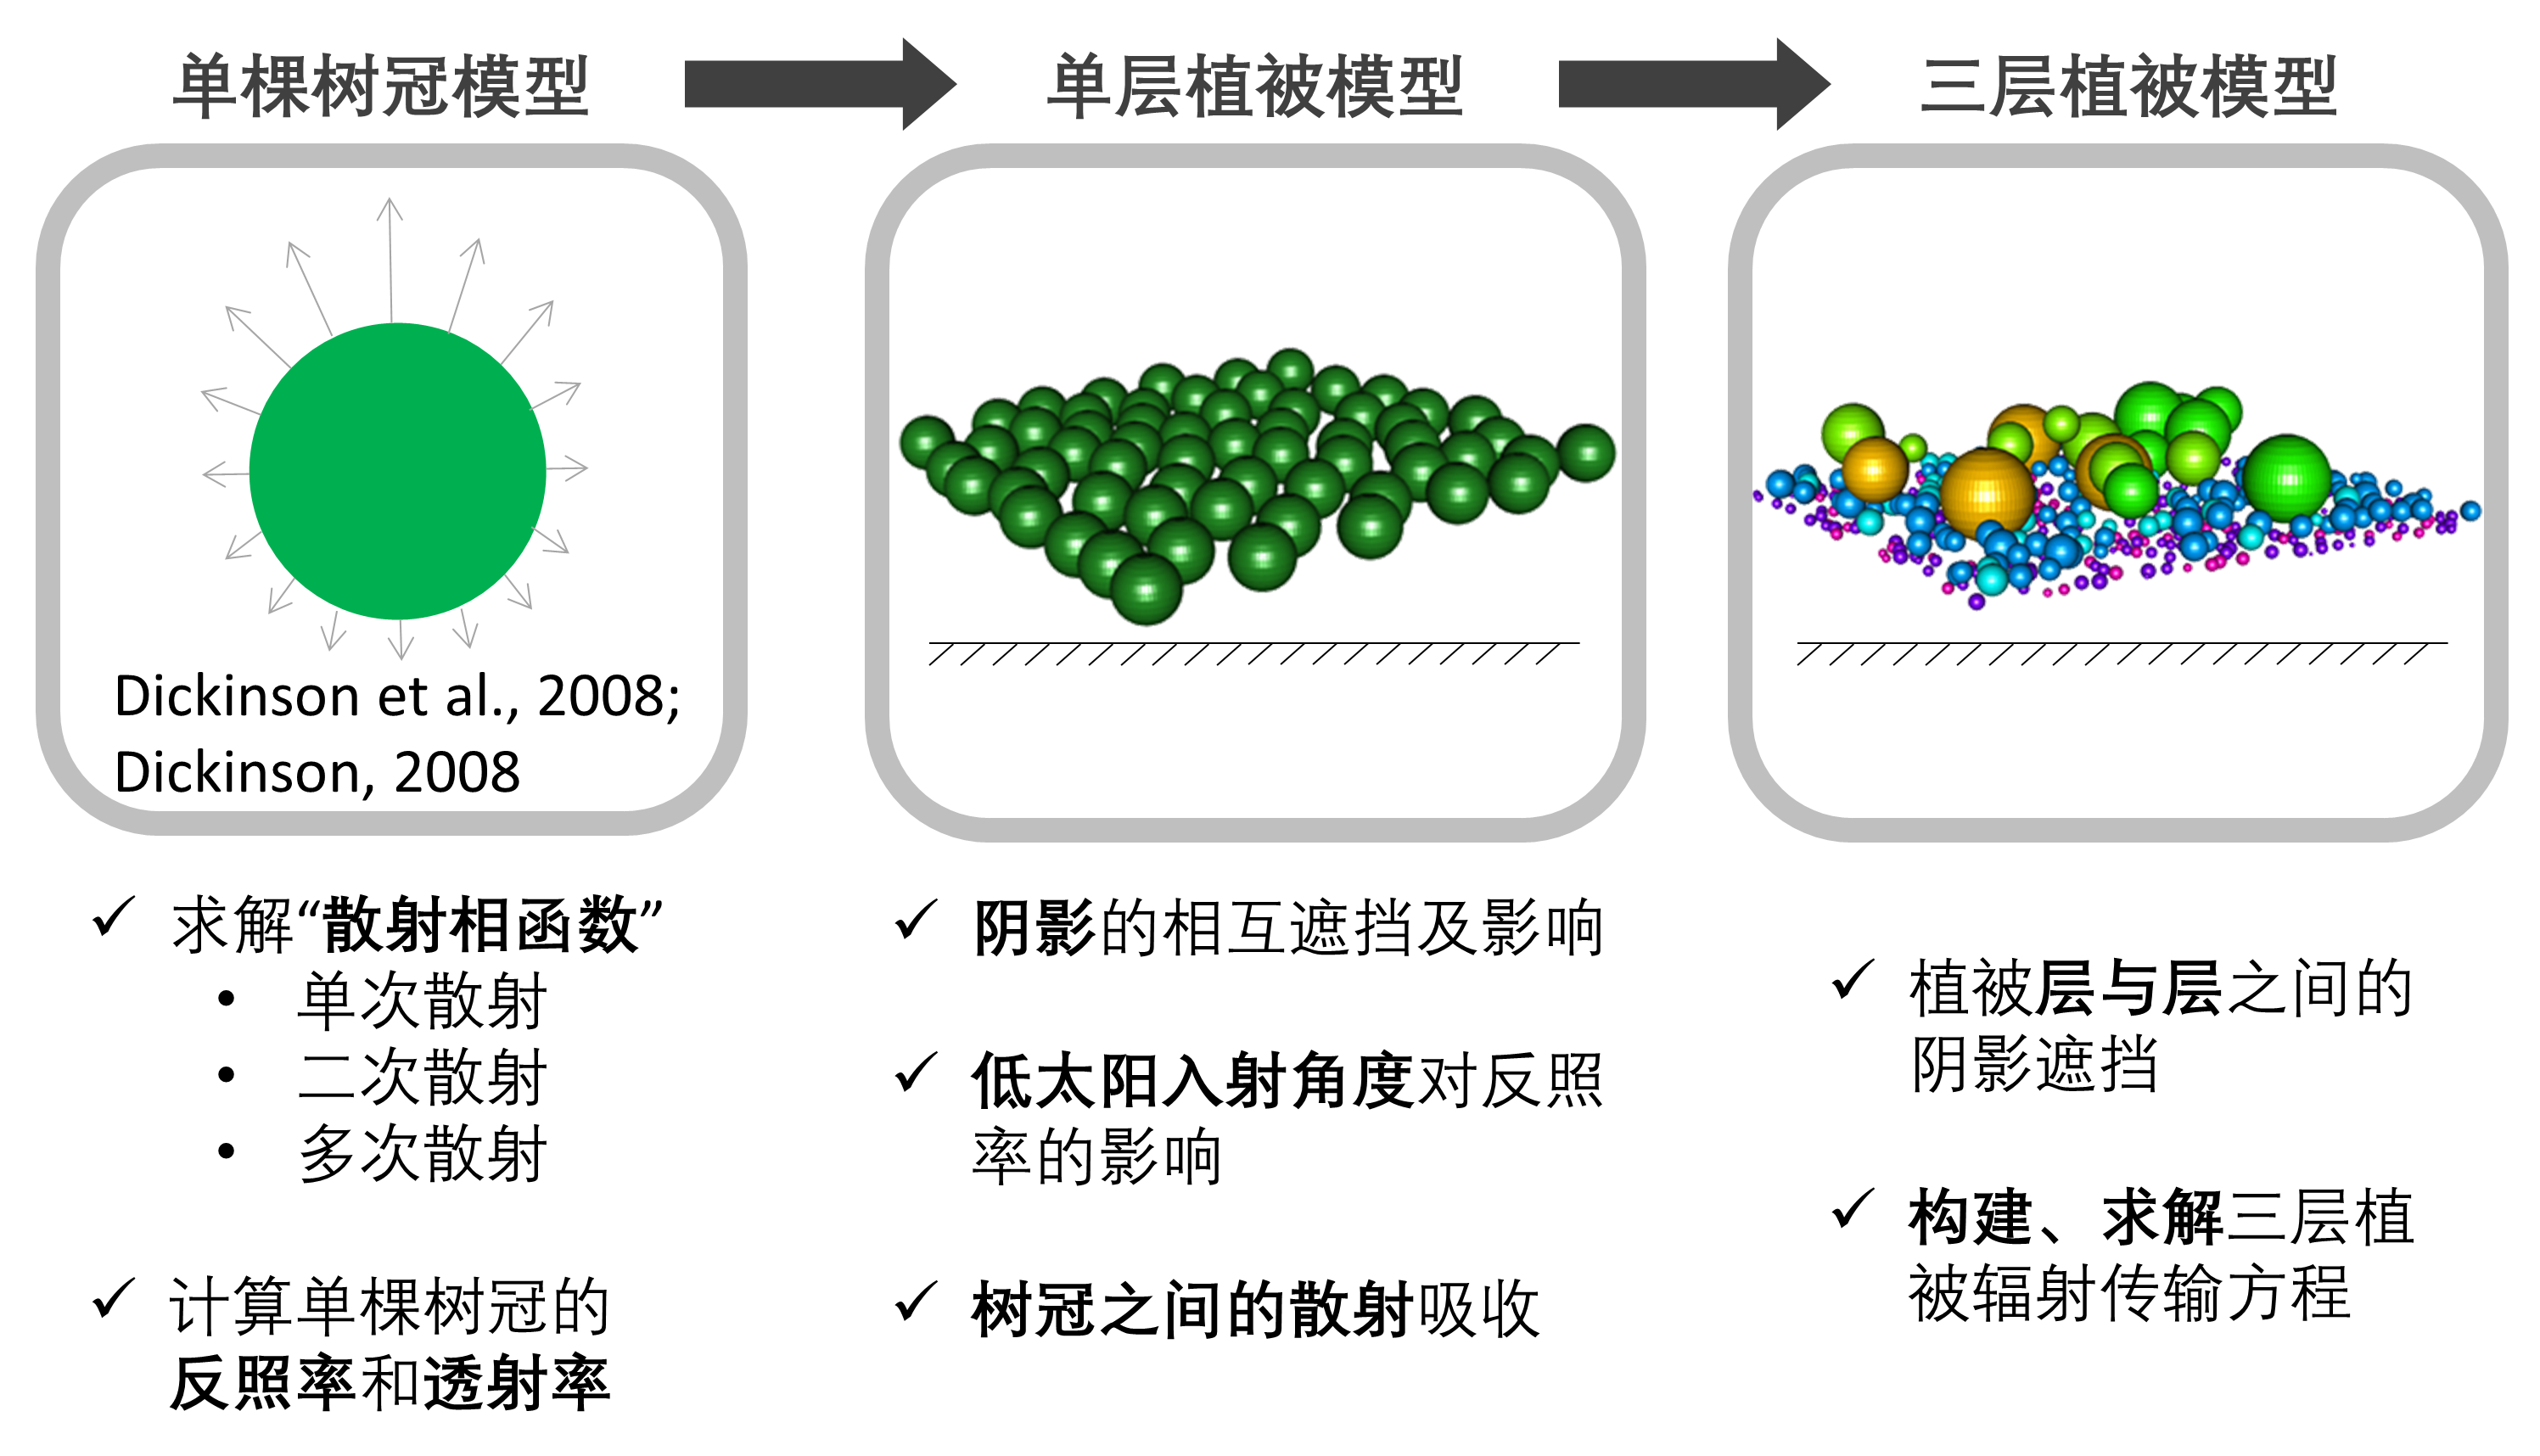
\includegraphics[width=0.95\columnwidth]{Figures/辐射过程及辐射通量计算/三维植被辐射传输模型基本框架.png}
\caption{三维植被辐射传输模型计算基本框架示意图}
\label{fig:三维植被辐射传输模型的基本框架}
\end{figure}
}


\subsection{单棵树冠模型}
单棵树冠模型基本假设是把植被树冠看成一个个的圆形球体,
叶片在其中均一分布,且叶倾角为球形分布(即$G$函数为1/2,$G$函数为单位体积叶面在某方向上的平均投影面积)。
首先考虑太阳辐射垂直入射,计算单棵球形植被的直射透射率$T_{d,s}\left(\tau\right)$:
{
\begin{figure}[htbp]
\centering
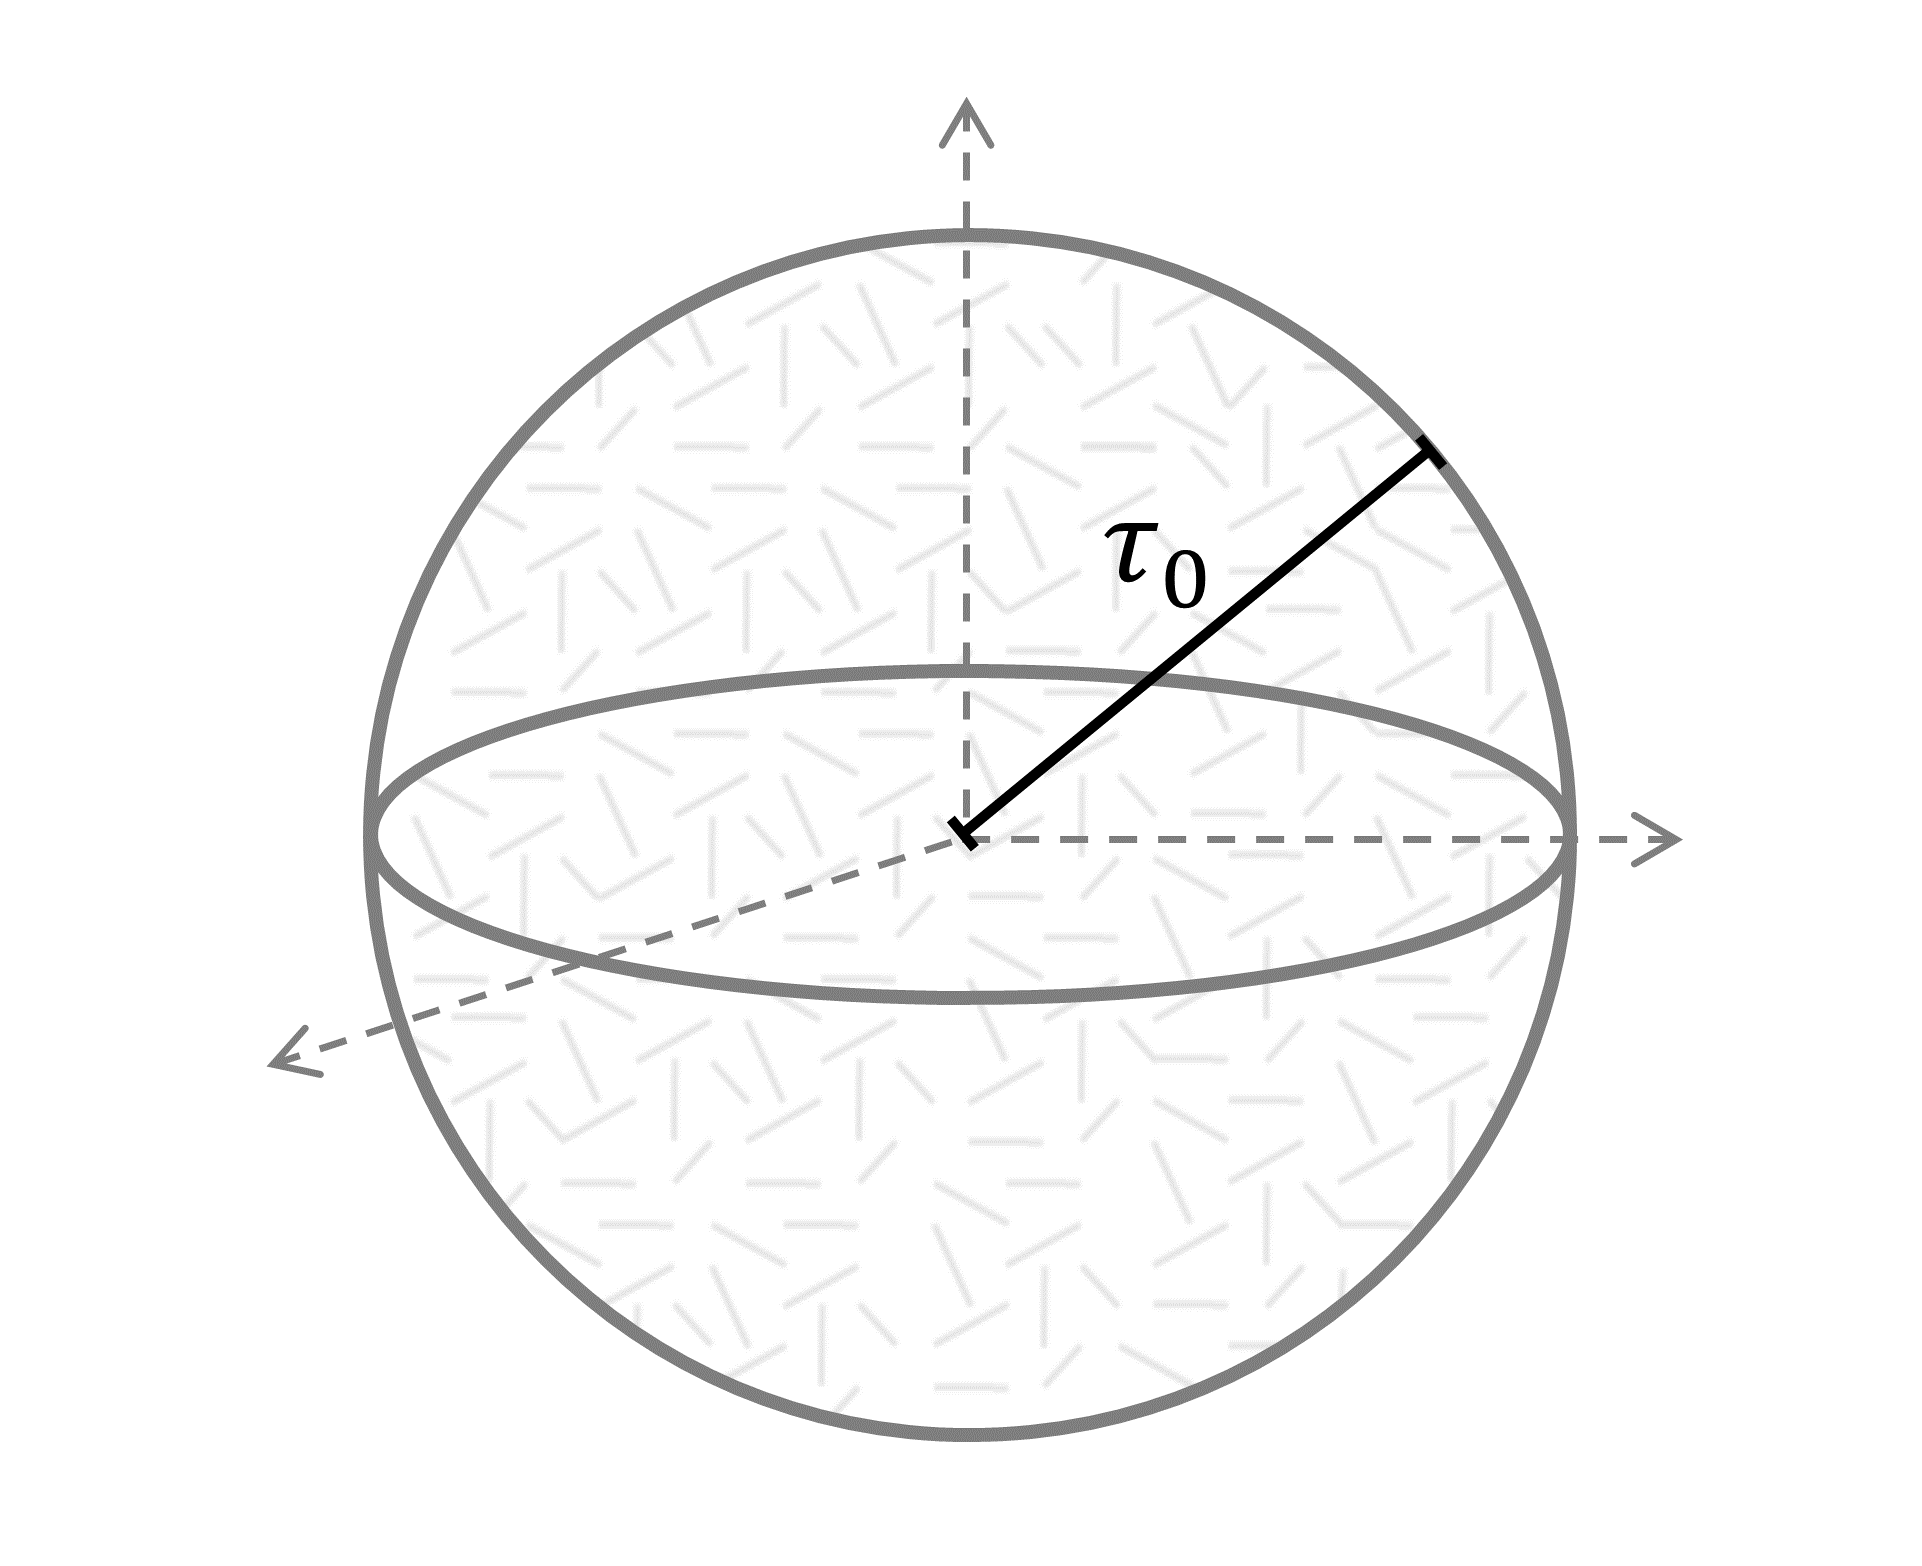
\includegraphics[width=0.6\columnwidth]{Figures/辐射过程及辐射通量计算/单棵树冠示意图.png}
\caption{单棵树冠示意图}
\label{fig:单棵树冠示意图}
\end{figure}
}
%
\begin{equation}\label{T_ds_tau}
T_{d, s}(\tau)=0.5 \tau^{-2}\left[1-(1+2 \tau) e^{-2 \tau}\right]
\end{equation}
$\tau$为沿球形植被半径长度的光学厚度参数(对于单棵树冠记为$\tau_0$,图~\ref{fig:单棵树冠示意图})。对单次散射的前向、后向散射相函数($\Phi_{1f}\left(\tau\right)$,$\Phi_{1b}\left(\tau\right)$)计算为:
\begin{align}
\Phi_{1 b}(\tau)=0.5\left[1-T_{d, s}(2 \tau)\right]
\Phi_{1 f}(\tau)=\tau^{-2}\left[1-\left(1+2 \tau+2 \tau^{2}\right) e^{-2 \tau}\right]
\end{align}
上式$\Phi_{1b}$和$\Phi_{1f}$为归一化结果(除以$0.25\omega^2/\pi$)。
二次散射前向、后向散射相函数($\Phi_{2f}\left(\tau\right), \Phi_{2b}\left(\tau\right)$)计算为:
\begin{align}
\Phi_{2 b}(\tau) & =a\left[\frac{1}{b+1}-\frac{1}{b-1} T_{d, s}(2 \tau)+\frac{2}{(b+1)(b-1)} T_{d, s}((b+1) \tau)\right] \\[2ex]
%
\Phi_{2 f}(\tau) & =a\left[\frac{2 b}{b^{2}-1} \Phi_{1 f}(\tau)-\left(\frac{1}{(b+1)^{2}}+\frac{1}{(b-1)^{2}}\right) T_{d, s}(\tau)+\frac{1}{(b-1)^{2}} T_{d, s}(b \tau)\right. \notag \\[1ex] 
&\qquad \left.\quad+\frac{1}{(b+1)^{2}} T_{d, s}((b+2) \tau)\right]
\end{align}
其中$a=0.70$,$b=1.74$,以上两式也为均一化的结果(除以$0.25\omega/\pi$)。假设单次和二次散射相函数从前向到后向强度线性变化,则总的单次散射和二次散射辐射计算为:
\begin{equation}
\Phi_{1 a}(\tau)=0.5\left[\Phi_{1 b}(\tau)+\Phi_{1 f}(\tau)\right]
\end{equation}
\begin{equation}
\Phi_{1 a}(\tau)=0.5\left[\Phi_{1 b}(\tau)+\Phi_{1 f}(\tau)\right]
\end{equation}
对于三次及以上散射相函数($\Phi_{3+}\left(\tau\right)$),假设其各向均一,利用二次散射后再次(与植被)碰撞的概率($p_2\left(\tau\right)$)进行计算:
\begin{equation}
\Phi_{3+}(\tau)=\frac{\omega p_{2}(\tau) \Phi_{2 a}(\tau)}{1-\omega p_{2}(\tau)}
\end{equation}
其中
\begin{equation}
p_{2}(\tau)=1-\frac{\Phi_{2 a}(\tau)}{1-T_{d, s}(\tau)-\Phi_{1 a}(\tau)}
\end{equation}
$\Phi_{3+}$为归一化结果(除以$0.25\omega^2/\pi$)。通过累加得到总的前向散射相函数($\Phi_f\left(\tau\right)$)及后向散射相函数($\Phi_b\left(\tau\right)$):
\begin{equation}
\Phi_{b}(\tau)=\frac{\omega}{4 \pi} \Phi_{1 b}(\tau)+\frac{\omega^{2}}{4 \pi}\left[\Phi_{2 b}(\tau)+\Phi_{3+}(\tau)\right]
\end{equation}
\begin{equation}
\Phi_{f}(\tau)=\frac{\omega}{4 \pi} \Phi_{1 f}(\tau)+\frac{\omega^{2}}{4 \pi}\left[\Phi_{2 f}(\tau)+\Phi_{3+}(\tau)\right]
\end{equation}
假设散射相函数的分布由后向到前向,沿天顶角呈线性变化(方位角水平均一),对任意散射出射角度$\theta_{out}$ (天顶角方向,$\mu_{out}=\cos{\theta_{out}}$),其总的散射相函数计算为:
\begin{equation}
\Phi_{\mu_{\mathrm{out}}}(\tau)=\Phi_{a}(\tau)+\mu_{\mathrm{out}} \Phi_{d}(\tau)
\end{equation}
其中$\Phi_a\left(\tau\right)=0.5\left[\Phi_b\left(\tau\right)+\Phi_f\left(\tau\right)\right]$,$\Phi_d\left(\tau\right)=0.5\left[\Phi_b\left(\tau\right)-\Phi_f\left(\tau\right)\right]$。
当太阳入射天顶角为$\theta$ ($\mu=\cos{\theta}$)时,对$\Phi_{\mu_{out}}\left(\tau\right)$进行积分计算,得到单株植物的反照率($\alpha_s\left(\mu,\tau\right)$)及漫射透射率($T_{i,s}\left(\mu,\tau\right)$)为:
\begin{equation}
\alpha_{s}(\mu, \tau)=2 \pi\left[\Phi_{a}(\tau)+0.5 \mu \Phi_{d}(\tau)\right]
\end{equation}
\begin{equation}
T_{i, s}(\mu, \tau)=2 \pi\left[\Phi_{a}(\tau)-0.5 \mu \Phi_{d}(\tau)\right]
\end{equation}
对于漫射辐射入射,模型考虑等效为直射入射为 60\textdegree 时的情形。


\subsection{单层植被模型}
单层植被模型假设球形树冠在水平方向上随机分布,但垂直投影不重叠。在植被覆盖率为$f_c$时,不考虑重叠的植被阴影面积为:
\begin{equation}
S_{0}=f_{c} / \mu
\end{equation}
若植被树冠的阴影可以随机重叠,根据概率理论模型,可以计算阴影面积为$1-e^{-f_c/\mu}$。但考虑在实际中,植被树冠在垂直投影上一般不重叠,修正的阴影面积为:
\begin{equation}\label{S_area}
S=\frac{1-e^{-f_{c} / \mu}}{1-f_{c} e^{-1 / \mu}}
\end{equation}
树冠阴影的重叠不仅直接影响阴影面积的大小,还增加了辐射穿过植被冠层的光学路径,单层植被的光学厚度把原有的单株植物光学厚度$\tau_0$等效修改为:
\begin{equation}\label{tau}
\tau=\tau_{0} S_{0} / S
\end{equation}
随着$f_c$的增加,植被树冠之间的散射吸收增加,为了计算这部分辐射,考虑最为简单的正六边形植被树冠分布(图~\ref{fig:散射吸收计算示意图}),容易计算得到红色树冠相对于绿色树冠的可视因子为:
\begin{equation}
V_{1}=\frac{1}{2}\left(1-\cos \theta_{v}\right)=\frac{1}{2}\left[1-\sqrt{1-\left(\frac{R}{L_{1}}\right)^{2}}\right]
\end{equation}
其中$\left(\frac{R}{L_{1}}\right)^{2}=\frac{\sqrt{3} f_{c}}{2 \pi}$。
考虑中心球周围6个树冠及稍远6个树冠对其散射辐射的吸收,可以得到总的可视因子为:
\begin{equation}
V=6 V_{1}+6 V_{2}=3\left[1-\sqrt{1-\frac{\sqrt{3} f_{c}}{2 \pi}}\right]+3\left[1-\sqrt{1-\frac{\sqrt{3} f_{c}}{6 \pi}}\right]
\end{equation}
假设可视立体角(在各个方位角方向)均一分布在中心球形树冠平行于地面的大圆上下$\pm\mu_v$的角度范围内,于是$\mu_v=V$。对球形树冠的散射相函数进行积分得到初次拦截的散射辐射为:
\begin{equation}
\frac{1}{2 \pi} \int_{0}^{2 \pi} \int_{-\mu_{v}}^{\mu_{v}} 2 \pi\left(\Phi_{a}+\mu \Phi_{d}\right) d \mu d \phi=4 \pi V \Phi_{a}
\end{equation}
利用再次碰撞概率概念估算总的树冠之间散射吸收为:
\begin{equation}
A_{c}=4 \pi V \Phi_{a}\left(\tau_{0}\right)\left[1-T_{d, s}\left(\tau_{0}\right)\right] \frac{1-\omega}{1-\omega p_{2}\left(\tau_{0}\right)}
\end{equation}
其中$\omega$为叶片单次散射反照率。

{
\begin{figure}[htbp]
\centering
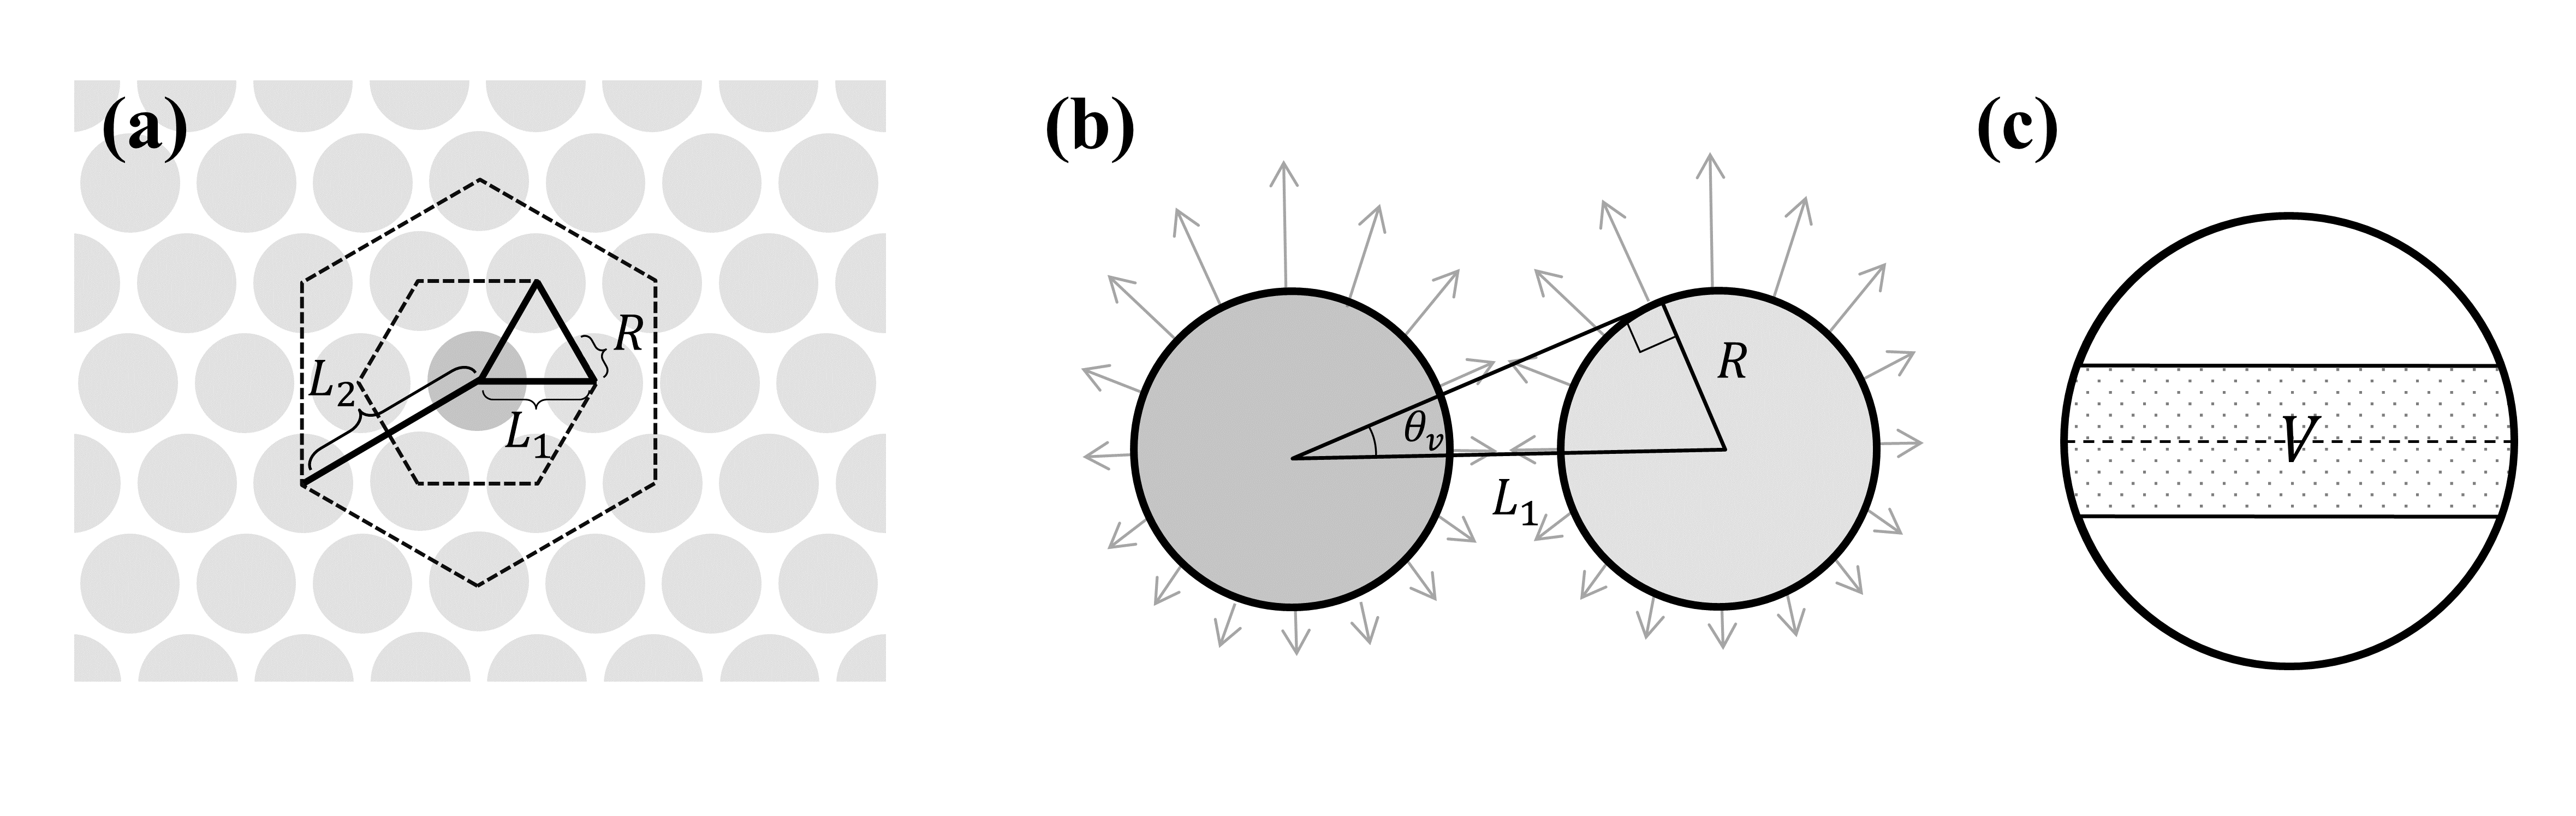
\includegraphics[width=0.95\columnwidth]{Figures/辐射过程及辐射通量计算/散射吸收计算示意图.png}
\caption{植被树冠之间散射吸收计算示意图}
\label{fig:散射吸收计算示意图}
\end{figure}
}

当太阳在较低的角度(高度角)入射时,植被树冠阴影重叠概率增大,树冠的光照面主要集中在顶部,此时的植被冠层类似于一维的情形,相对于球形植被计算结果,$albedo$会有所增加。
我们利用 \citet{dickinson1983land} 对一维植被单次散射的分析结果,计算对$albedo$的增量为:
\begin{equation}
\alpha_{L}=(N-1) \alpha_{s}\left(\mu=1, \tau_{0}\right) f_{c}\left(\frac{1}{s}-\frac{1}{s_{0}}\right)
\end{equation}
其中$N$表示相对于垂直入射植被冠层时$albedo$的倍数,是太阳入射角度的函数:
\begin{equation}
N=\frac{1+2 \beta_{2}}{1+2 \beta_{2} \mu}
\end{equation}
其中$\beta_2=\left(1-\omega\right)^\frac{1}{2}(1-\omega+2\omega\beta)$。
植被树冠之间的吸收增量会使$albedo$和漫射透射减少,低入射角度对$albedo$的增量会降低植被的吸收和漫射透射,把以上增加的部分均一分配到减少项,
得到单层植被$albedo$ ($\alpha$),植被直射透射($T_d$)漫射透射($T_i$)及吸收($A$)为:
\begin{equation}
\alpha=\alpha_{s}(\mu, \tau)+\alpha_{L}-0.5 A_{c}
\end{equation}
\begin{equation}
T_{i}=T_{i, s}(\mu, \tau)-0.5 \alpha_{L}-0.5 A_{c}
\end{equation}
\begin{equation}
A=1-\alpha-T_{i}-T_{d}
\end{equation}
对于漫射辐射入射,同样考虑等效为直射入射为 60\textdegree 的情形。

以上的推导均基于正球体和球形叶倾角分布函数情况下,下面将对椭球体和非球形叶倾角分布进行订正。

\textit{1) 椭球树冠}

对于椭球体树冠(图~\ref{fig:椭球体树冠}a),其对辐射计算的影响主要有3个方面(均可等效看成对光学厚度$\tau$的影响):
\begin{enumerate}
    \item 椭球相对于正球的拉升/压缩影响单位长度的光学厚度(因叶密度改变);
    \item 几何形状的改变造成光学路径的长度的改变;
    \item 阴影面积重合部分改变对光学厚度的影响。
\end{enumerate}

 {
    \begin{figure}[htbp]
    \centering
    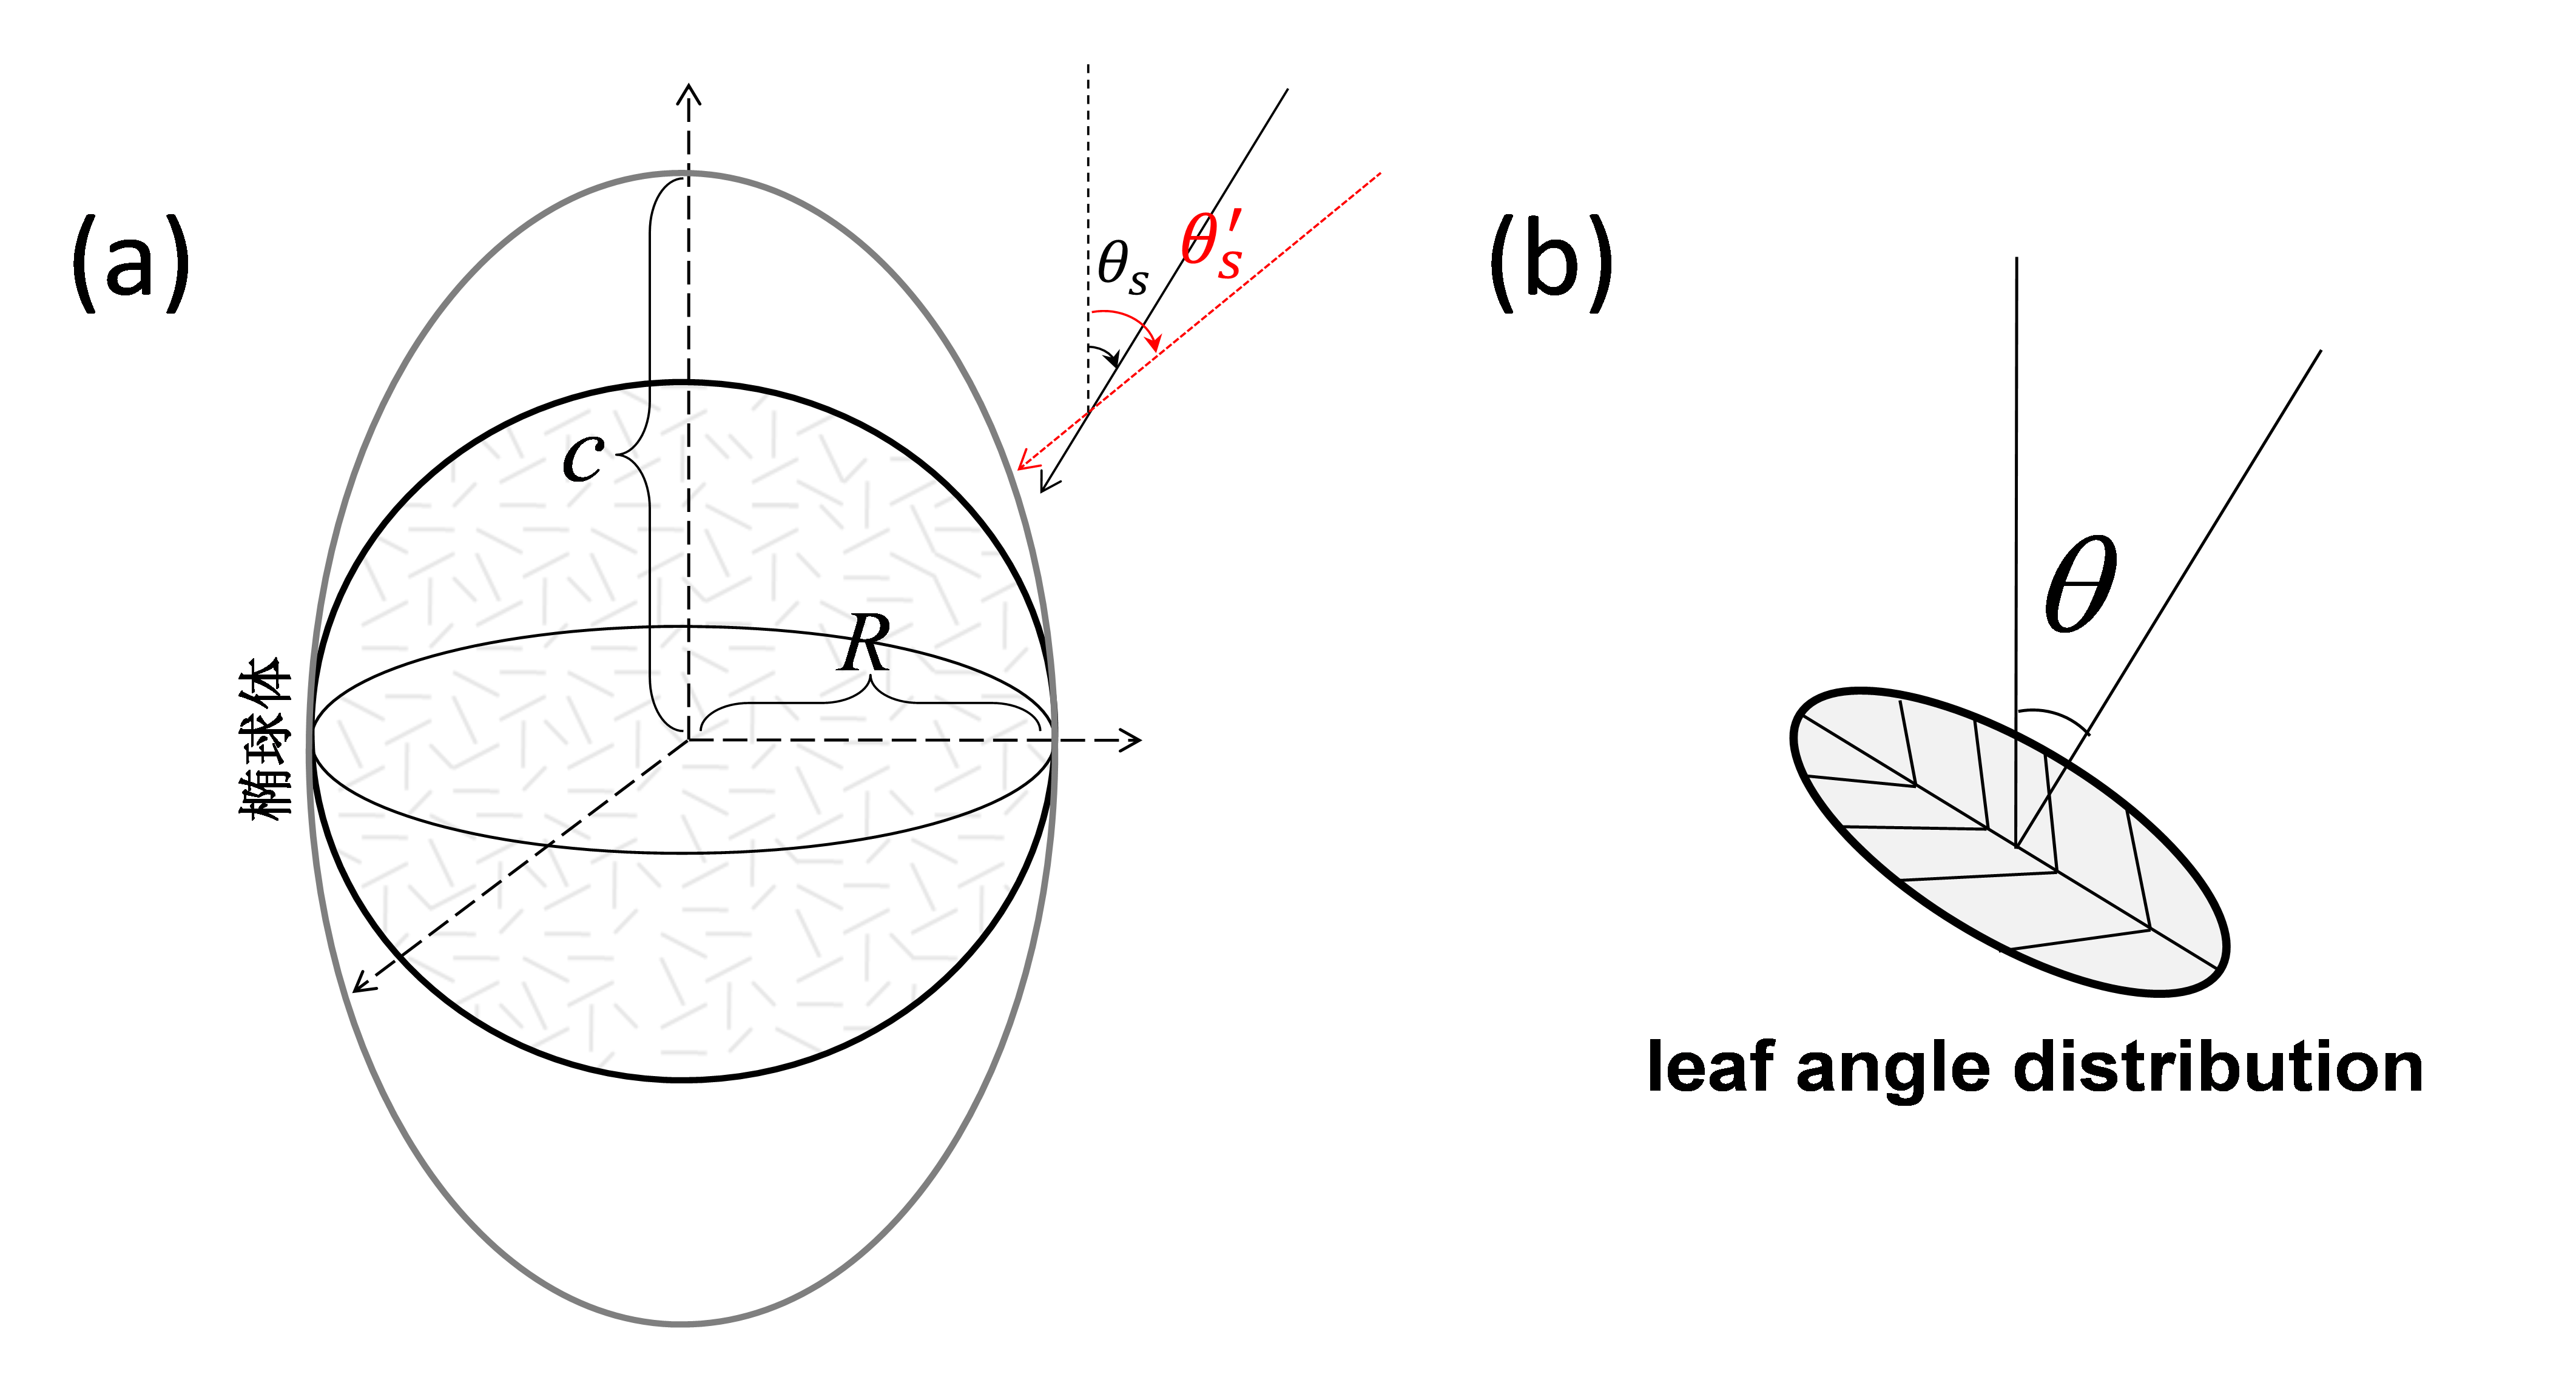
\includegraphics[width=0.8\columnwidth]{Figures/辐射过程及辐射通量计算/椭球体树冠.png}
    \caption{(a) 树冠形状从正球体扩展到椭球体;(b) 考虑叶倾角分布}
    \label{fig:椭球体树冠}
    \end{figure}
    }

椭球体可能看成是正球体在垂直方向$y$轴的拉伸,在椭球坐标系下的$y$,
在正球体坐标系下就变成$y^\prime$。让$c$为椭球体半轴长(沿$y$轴),$R$为球体水平方向的半径,可以得到:
\begin{equation}
y^{\prime}=\frac{R}{c} y, \text { and } x^{\prime}=x
\end{equation}
于是有$\tan{\theta_s^\prime}=\frac{x^\prime}{y^\prime}=\frac{c}{R}{\tan{\theta}}_s$,
椭球体在地面的投影面积即为$\pi R^2/\cos{\theta_s^\prime}$。将$\theta_s^\prime$进行替换,得到阴影面积计算公式为:
\begin{equation}\label{SSS}
\begin{aligned} S &=\frac{\pi R^{2}}{\cos \theta_{s}^{\prime}} \\ &=\frac{\pi R^{2}}{\cos \theta_{s} 
\sqrt{\frac{1}{c r^{2} \sin ^{2} \theta_{s}+\cos ^{2} \theta_{s}}}} \end{aligned}
\end{equation}
式中$cr=c/R$。可以看出,当$c=R$时,与正球体计算一致。$\cos{\theta_s}$与$\cos{\theta_s^\prime}$的关系从公式 (\ref{SSS}) 很容易看出。%caution


椭球体对$\tau$影响的三个方面,我们用$c_1$, $c_2$, $c_3$三个系数表示。对于$c_1$,很容易得到$c_1=1/cr$。$c_2$的计算稍微复杂一点,可表达为:
\begin{equation}
\begin{aligned} c_2 &=\frac{y}{y^{\prime}} \cdot \frac{\cos \theta_{s}^{\prime}}{\cos \theta_{s}}=
    c r \sqrt{\frac{1}{c r^{2} \sin ^{2} \theta_{s}+\cos ^{2} \theta_{s}}} \\ &=
    \sqrt{\frac{c^{2}}{c^{2} \sin ^{2} \theta_{s}+R^{2} \cos ^{2} \theta_{s}}} \end{aligned}
\end{equation}
对于$c_3$,实际上是计算在等效的天顶角$\theta_s^\prime$下,考虑阴影重叠后的等效$\tau$,其计算表达式在公式(\ref{tau})已给出。

\textit{2) 非球形叶倾角分布}

对于球形分布函数,前面已提到$G=0.5$;对于参数为$\chi_L$的叶倾角分布,
可以利用公式(\ref{Gmu})计算得到特定太阳入射角的$G\left(\theta_s\right)$。
对于光学厚度相对原始$\tau$的比例系数为$c_4=G\left(\theta_s\right)/0.5$。

综合以上几个方面,即把光学厚度参数$\tau$修改为$c_1c_2c_3c_4\tau$,
然后代入直射透射计算公式,便可得到单层植被的直射透射率$T_d^\prime$,
假设在正球体情况下的直射透射率为$T_d$,在不考虑椭球形状和叶倾角分布情况下,能量守恒等式表达为:
\begin{equation}
\alpha+A+T_{d}+T_{i}=1
\end{equation}
定义散射/吸收辐射的订正因子为$\frac{1-T_d^\prime}{1-T_d}$,把由直射透射引起的截获辐射量变化考虑为$S$和$A$的改变,即分别修正为$\frac{1-T_d^\prime}{1-T_d}S$和$\frac{1-T_d^\prime}{1-T_d}A$,新修正的各个变量同样满足能量守恒方程:
\begin{equation}
\frac{1-T_{d}^{\prime}}{1-T_{d}} \alpha+\frac{1-T_{d}^{\prime}}{1-T_{d}} A+T_{d}^{\prime}+\frac{1-T_{d}^{\prime}}{1-T_{d}} T_{i}=1
\end{equation}
再考虑对单层植被辐射散射/吸收特性的改变之外,树冠的形状改变还影响地面的阴影计算,对于单层植被,可以利用等效的$\cos{\theta_s^\prime}$值(即$\cos{\theta_s}\sqrt{\frac{1}{{cr}^2\sin^2{\theta_s}+\cos^2{\theta_s}}}$)。 
若考虑植被与地面之间的多次散射,初次透射到地面的辐射$T$ ($T=1-S+S\left(T_d+T_i\right)$) 经过地面的反射(地表反射率$r_g$),再次与植被冠层反射到达地面,如此反复。到达地面的辐射为一等比数列,其比例因子为$q=r_gS^\ast\alpha^\ast$,上标“$\ast$”表示漫射辐射入射时相应变量值(下同)。
由于地表与植被之间多次散射的植被吸收$A^m=\frac{Tr_gS^\ast A^\ast}{1-q}$,总的植被吸收($\left[A\right]$),透射率($\left[T\right]$),地表吸收($\left[G\right]$)和地表$albedo$ ($\left[\alpha\right]$)计算如下:
\begin{equation}
[A]=S A+A^{m}
\end{equation}
\begin{equation}
[T]=\frac{T}{1-q}
\end{equation}
\begin{equation}
[G]=\left(1-r_{g}\right)[T]
\end{equation}
\begin{equation}
[\alpha]=1-[A]-[G]
\end{equation}


\subsection{三层植被模型}
三层植被模型的假设在单株植物模型和单层植被模型的基础上,认为层与层之间的树冠垂直投影不重叠,
每层植被树冠半径$(R$)和树冠中心高度($h$)相同(图~\ref{fig:三层植被结构示意图})。
若某层植被含有多种PFT,则该层的$f_c$为所含PFT各自$f_c$的累加,
植被参数的层属性(包括$LAI$、$R$、$h$及叶片光学属性)为所含PFT的$f_c$加权平均。

层与层之间的阴影重叠对直射辐射的吸收影响很大,特别是对于较高吸收率的可见光波段。
对于阴影的重叠,3D模型假设高层树冠的“自身阴影”(在低层植被的阴影与其自身垂直投影的重叠区域)
不与低层树冠的阴影重叠(如图~\ref{fig:三层植被结构示意图}所示的$S_{12}$、$S_{13}$和$S_{23}$)。除此之外,层与层之间的阴影可以随机重叠。%
{
\begin{figure}[htbp]
\centering
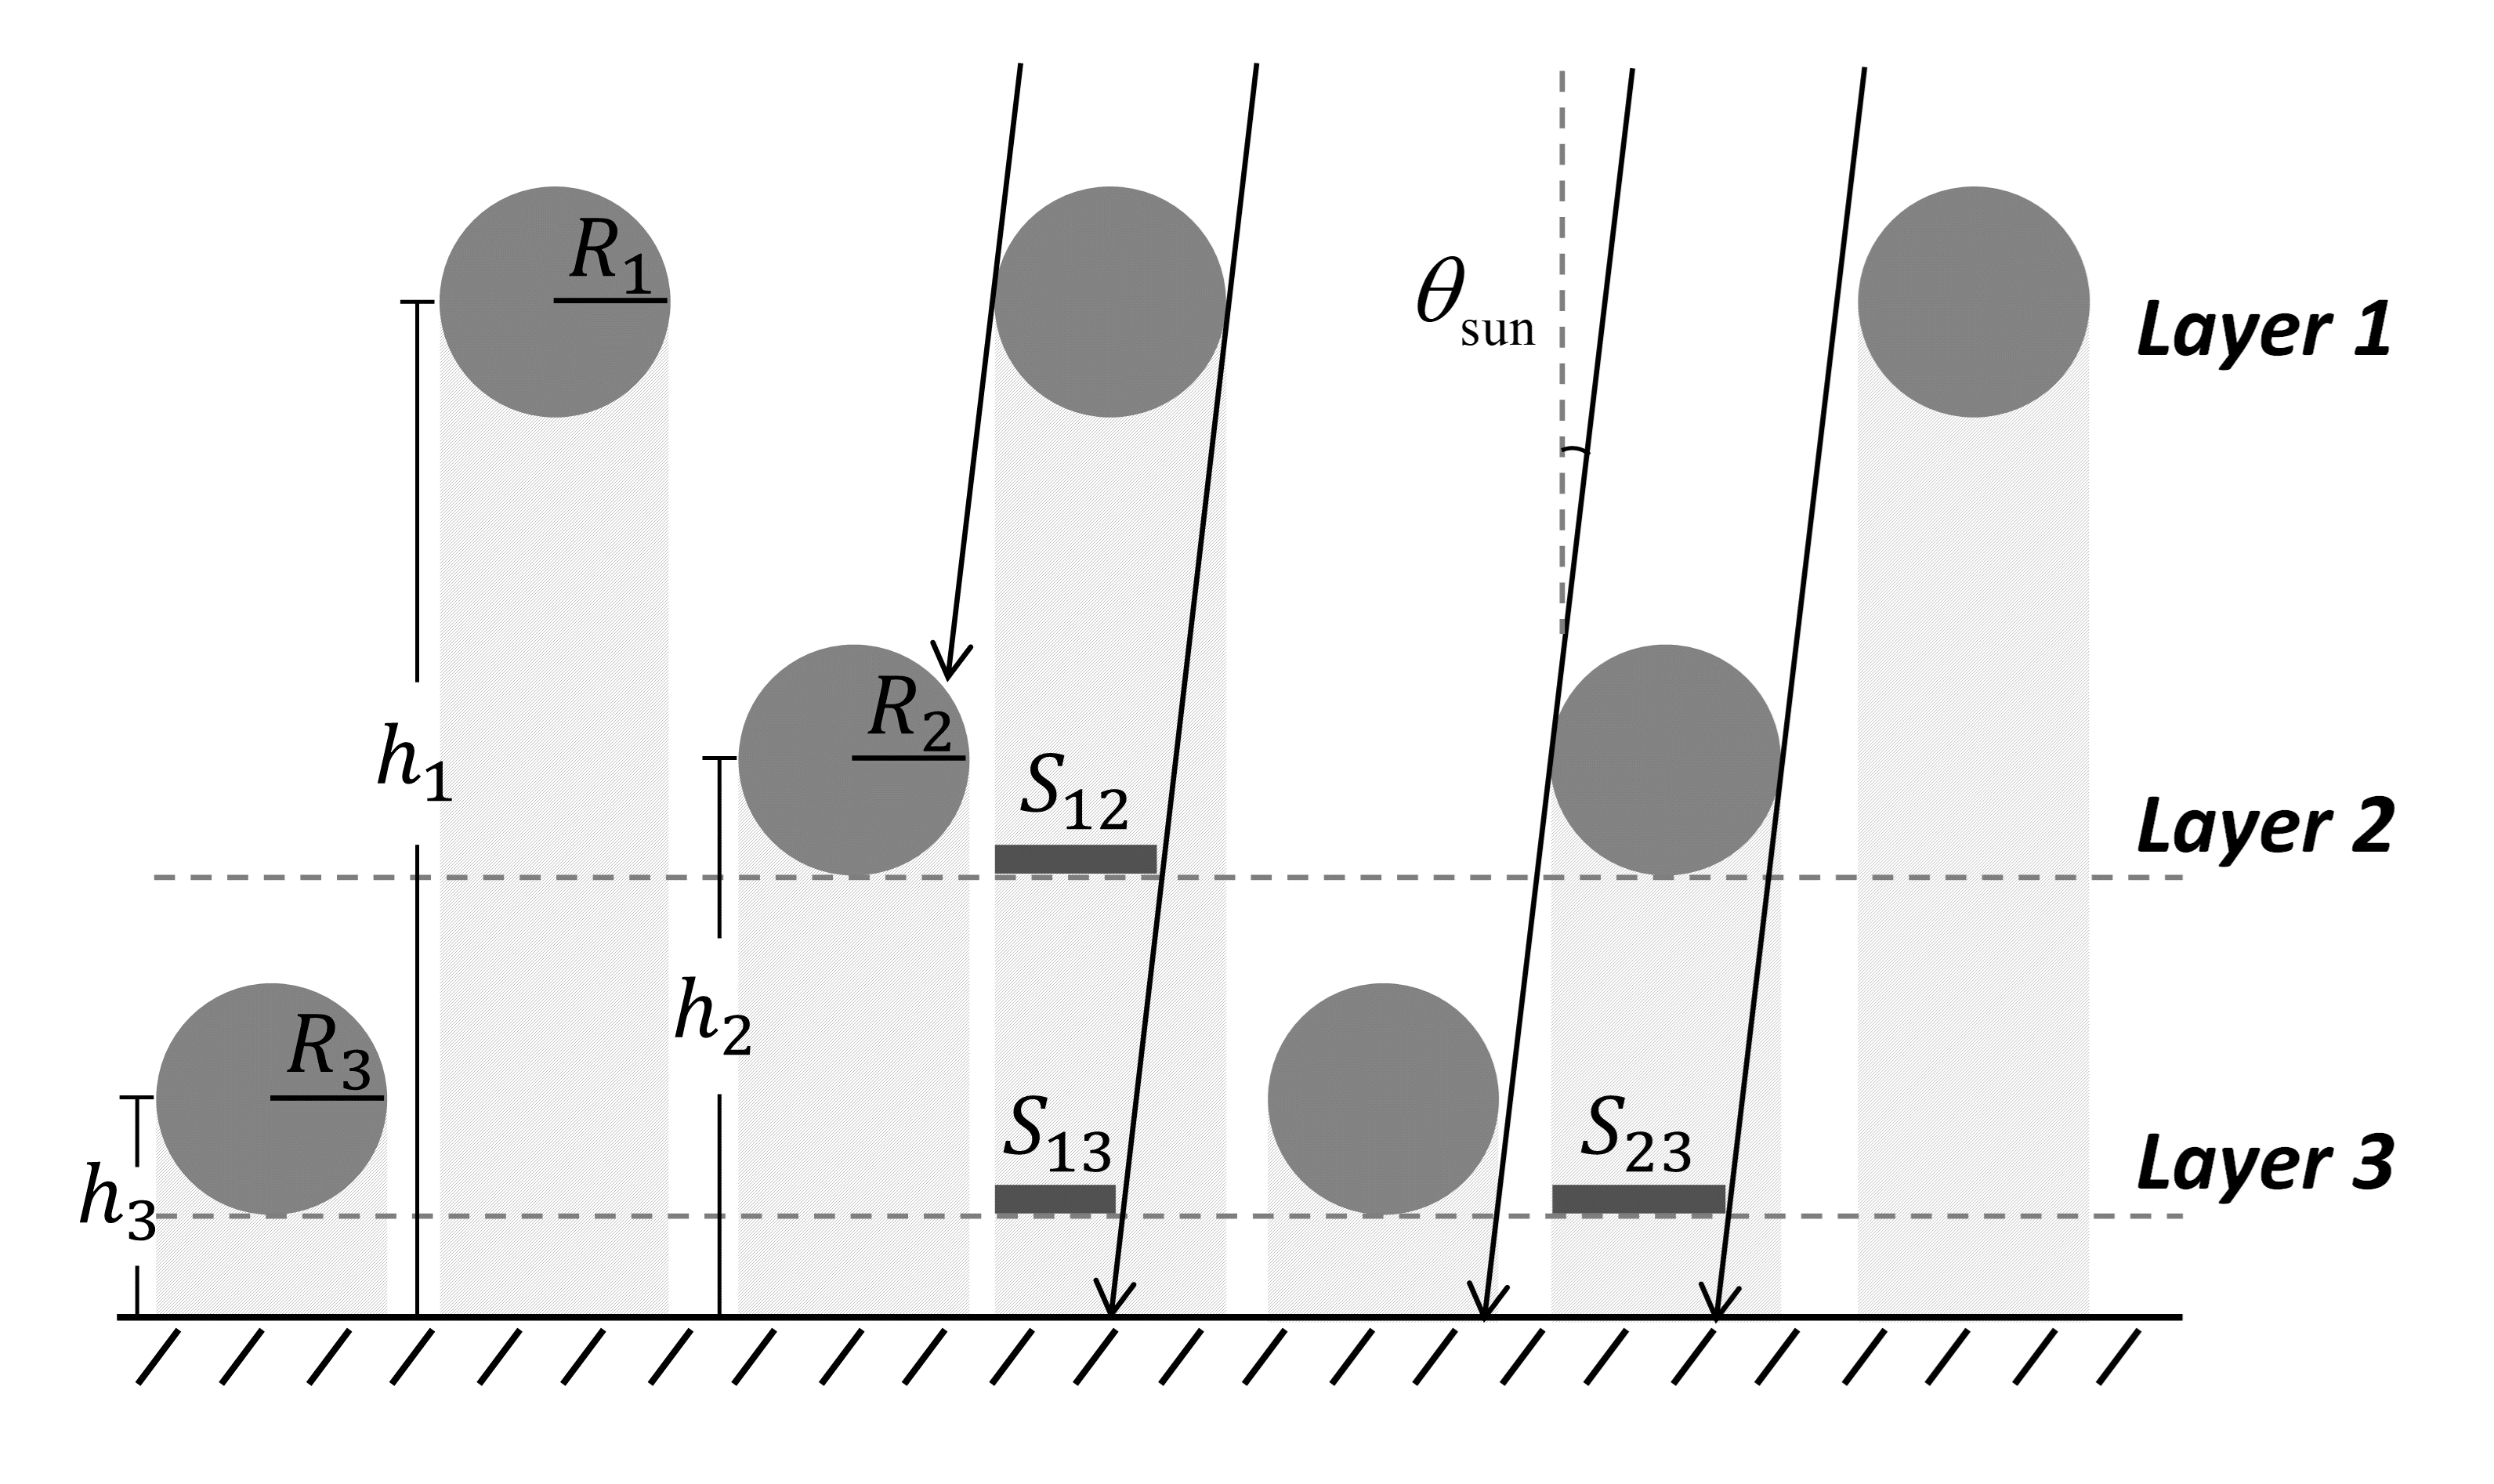
\includegraphics[width=0.8\columnwidth]{Figures/辐射过程及辐射通量计算/三层植被结构示意图.png}
\caption[三层植被直射辐射传输示意图]{三层植被直射辐射传输示意图。[注:图中树冠大小和形状仅作为示意,每层植被树冠大小不必一致,形状不必为正球体]}
\label{fig:三层植被结构示意图}
\end{figure}
}
用$I_{\left[from\right]\rightarrow\left[to\right]}$表示层与层之间的直射辐射直射透射量,
$S[n]$表示第$n$层植被的阴影面积,$Td$,$[n]$为第$n$层植被的直射辐射直射透射率,可以计算从天空($sky$),
不穿过植被,到达每层植被及地面的初始直射辐射为(为了与三维植被辐射传输模型引文~\citep{yuan20143d} 吻合
,这里保留了植被分层计数从上到下1-3的方式,但之后三维植被长波辐射传输
、三维植被湍流交换过程等采用从上至下3-1的编号,与代码一致):
\begin{equation}
\begin{aligned} I_{0 \rightarrow 1} &=S_{1} \\ I_{0 \rightarrow 2} &=\left(1-S_{1}+S_{12}\right) S_{2} \\ 
    I_{0 \rightarrow 3} &=\left[1-\left(S_{1}-S_{13}\right)-\left(S_{2}-S_{23}\right)+\left(S_{1}-S_{12}\right)\left(S_{2}-S_{23}\right)\right] S_{3} \\ 
    I_{0 \rightarrow g} &=1-S_{1}-S_{2}-S_{3} \\ &+\left(S_{1}-S_{12}\right) S_{2}+\left(S_{1}-S_{13}\right) S_{3}+\left(S_{2}-S_{23}\right) S_{3} \\
     &-\left(S_{1}-S_{12}\right)\left(S_{2}-S_{23}\right) S_{3} \end{aligned}
\end{equation}
到达L1的直射辐射可以继续直射透射到达下层,计算为:
\begin{equation}
\begin{aligned}
I_{1 \rightarrow 2} &=T_{d, 1}\left(S_{1}-S_{12}\right) S_{2} \\[1ex]
I_{1 \rightarrow 3}&=T_{d, 1}\left[S_{1}-S_{13}-\left(S_{1}-S_{12}\right)\left(S_{2}-S_{23}\right)\right] S_{3} \\[1ex]
I_{1 \rightarrow g} &=T_{d, 1}\left[S_{1}-\left(S_{1}-S_{12}\right) S_{2}-\left(S_{1}-S_{13}\right) S_{3}+\left(S_{1}-S_{12}\right)\left(S_{2}-S_{23}\right) S_{3}\right]
\end{aligned}
\end{equation}
同理可以得到:
\begin{equation}
\begin{aligned}
I_{2 \rightarrow 3} & =T_{d, 2}\left[I_{0 \rightarrow 2}+I_{1 \rightarrow 2}\right] \frac{\left(S_{2}-S_{23}\right) S_{3}}{S_{2}} \\[1ex]
I_{2 \rightarrow g} & =T_{d, 2}\left[I_{0 \rightarrow 2}+I_{1 \rightarrow 2}\right] \frac{S_{2}-\left(S_{2}-S_{23}\right) S_{3}}{S_{2}} \\[1ex] 
I_{3 \rightarrow g} &=T_{d, 3}\left[I_{0 \rightarrow 3}+I_{1 \rightarrow 3}+I_{2 \rightarrow 3}\right]
\end{aligned}
\end{equation}

累加以上结果,可以计算到达每层的初始直射辐射为:
\begin{equation}
\begin{array}{l}I_{1}=I_{0 \rightarrow 1} \\ I_{2}=I_{0 \rightarrow 2}+I_{1 \rightarrow 2} \\ 
    I_{3}=I_{0 \rightarrow 3}+I_{1 \rightarrow 3}+I_{2 \rightarrow 3} \\ 
    I_{g}=I_{0 \rightarrow g}+I_{1 \rightarrow g}+I_{2 \rightarrow g}+I_{3 \rightarrow g}\end{array}
\end{equation}
第$n$层植被的直射辐射直射吸收量为:
\begin{equation}
I_{n}\left(1-T_{d, n}\right)(1-\omega)
\end{equation}
第$n$层植被的太阳直射照射面积($p_{sun}$)计算为:
\begin{equation}
p_{sun}=I_{n} / S_{n}
\end{equation}
上式表明每层植被并不是100\%的被太阳直射照射,该参数将会用于修正植被光照叶面积指数(图~\ref{fig:三层植被辐射传输计算示意图})。
{
\begin{figure}[htbp]
\centering
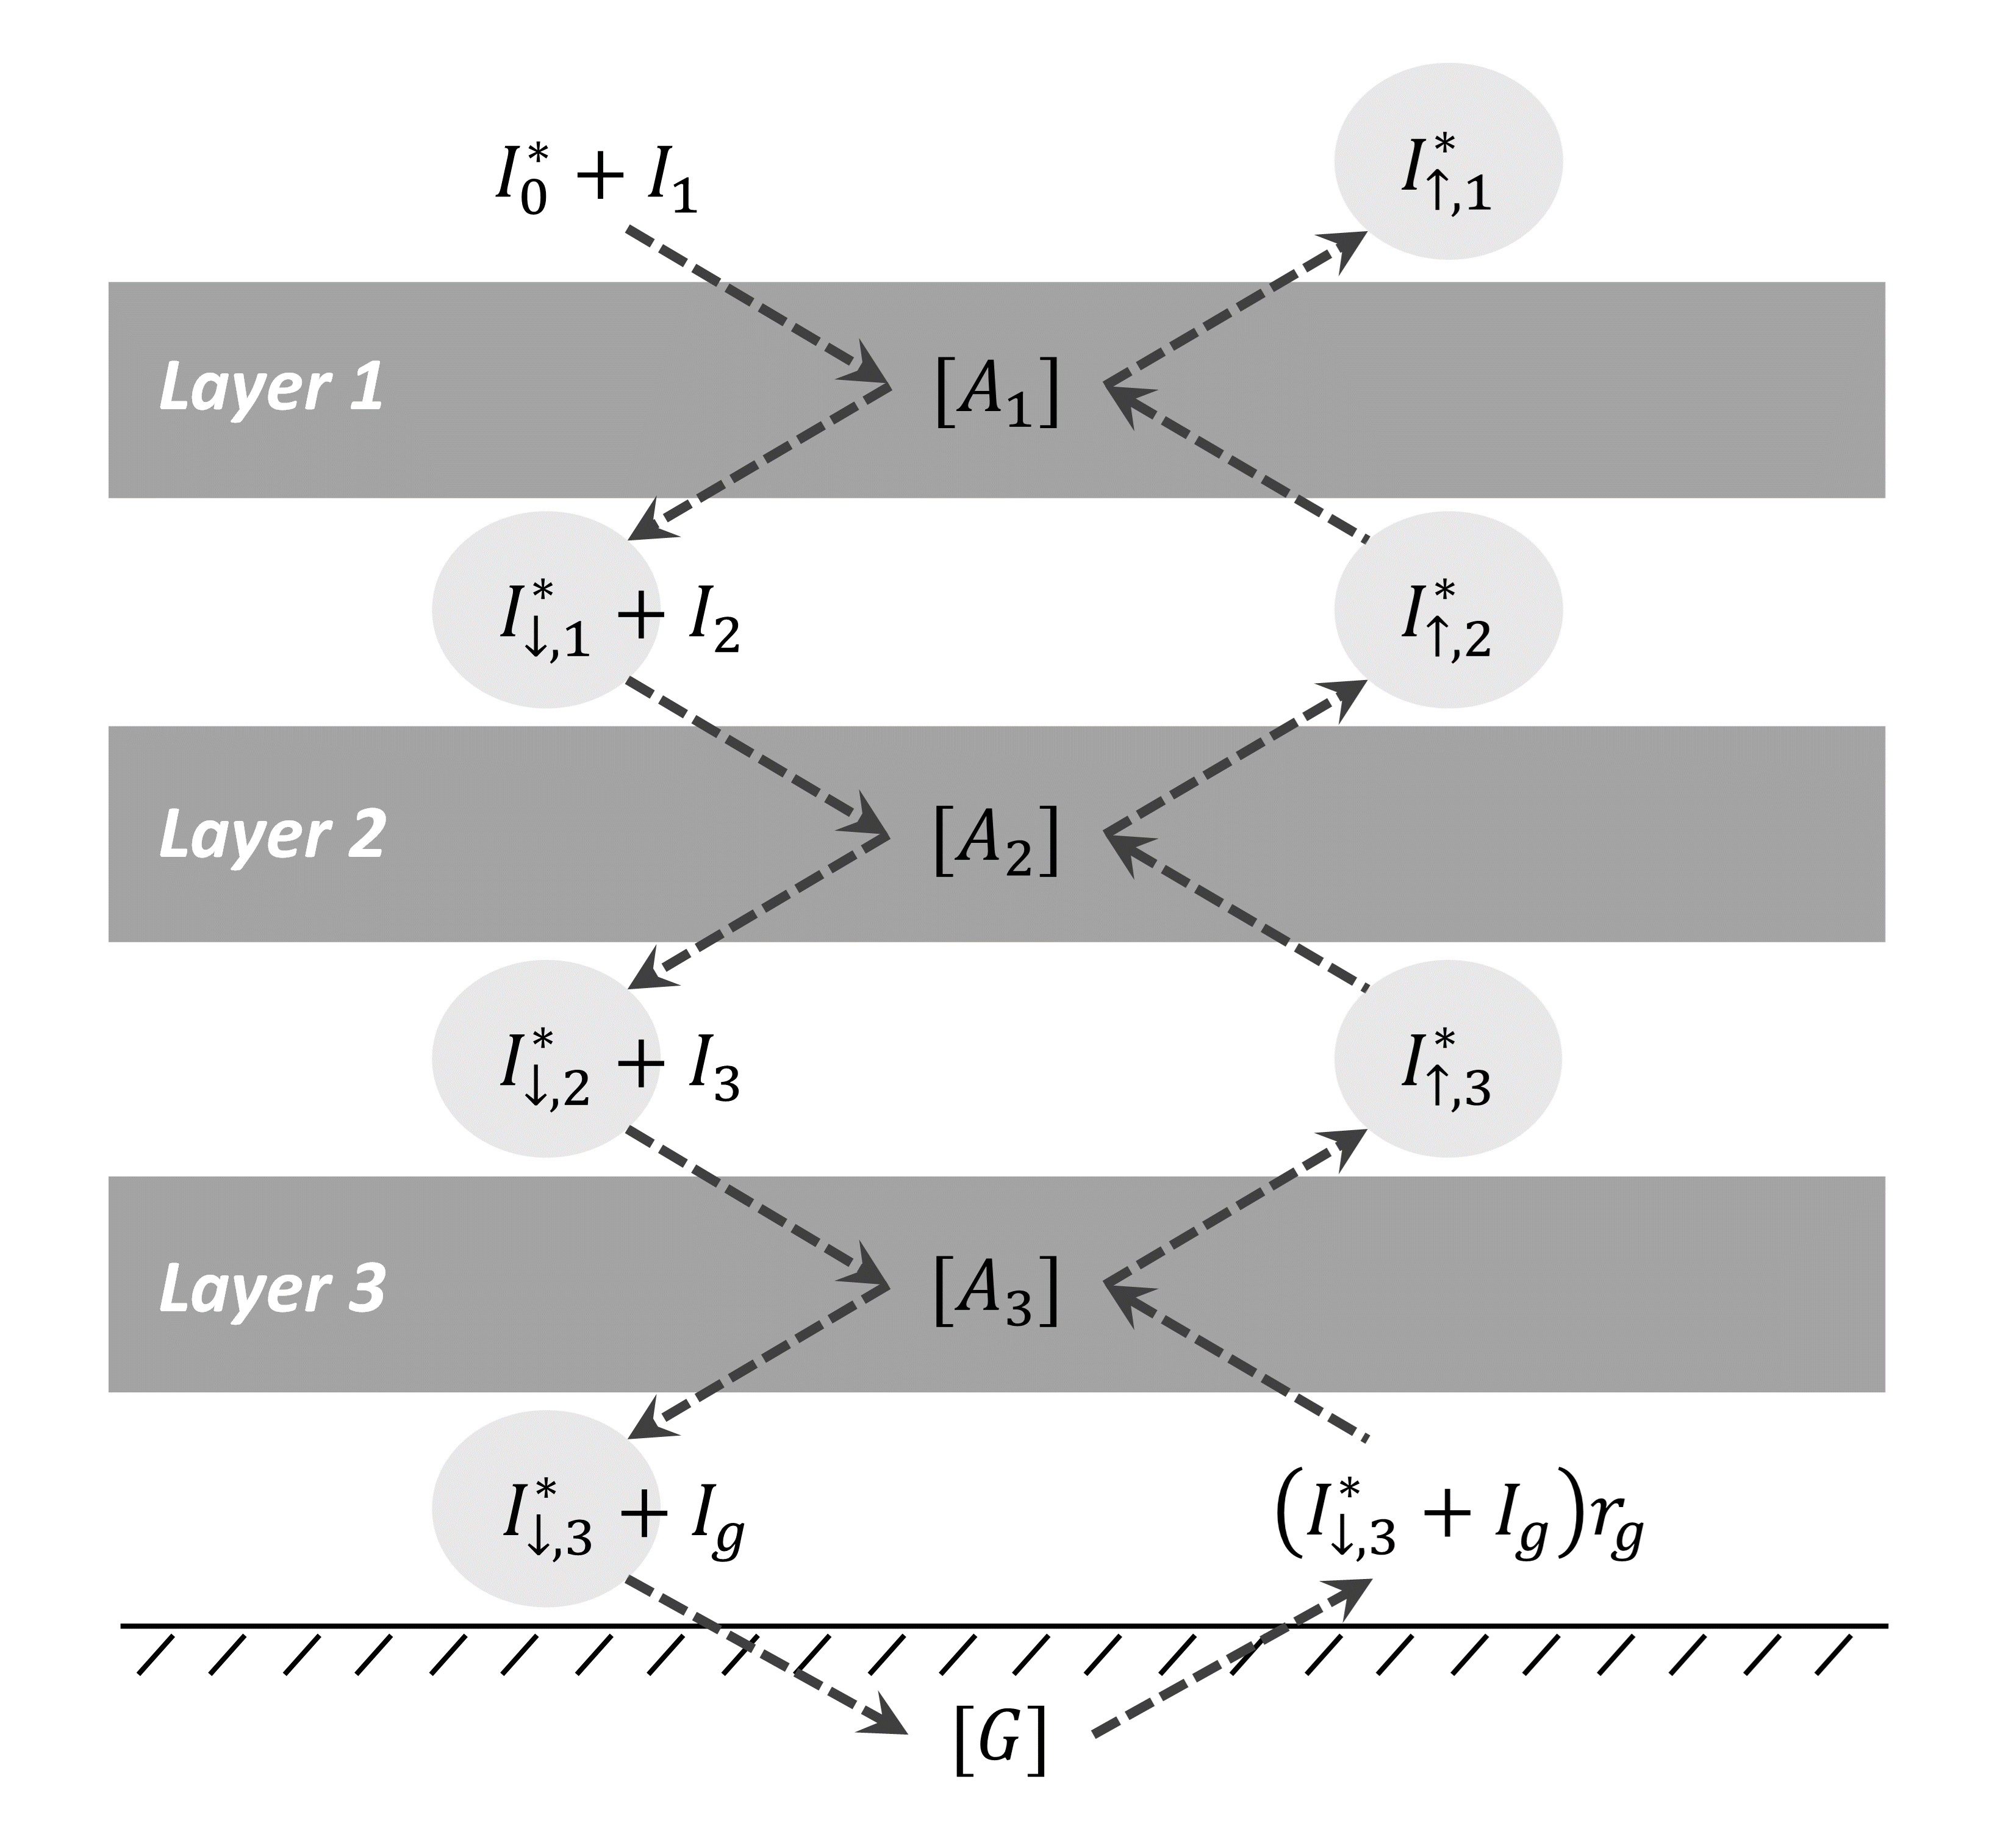
\includegraphics[width=0.7\columnwidth]{Figures/辐射过程及辐射通量计算/三层植被辐射传输计算示意图.png}
\caption{三层植被辐射传输计算示意图}
\label{fig:三层植被辐射传输计算示意图}
\end{figure}
}
三层植被模型的计算采用线性方程组进行计算。六个变量,$I_{\uparrow,1}^\ast$, $I_{\downarrow,1}^\ast$, $I_{\uparrow,2}^\ast$, $I_{\downarrow,2}^\ast$, $I_{\uparrow,3}^\ast$ 和 $I_{\downarrow,3}^\ast$,
被选择作为未知变量。他们分别表示每层植被的向上/向下漫射辐射通量,可以表示为:
\begin{equation}
\begin{aligned}
I_{\uparrow, 1}^{*} & =I_{1} \alpha_{1}+I_{\uparrow, 2}^{*} S_{1}^{*} T_{i, 1}^{*}+I_{\uparrow, 2}^{*}\left(1-S_{1}^{*}\right)+I_{0}^{*} S_{1}^{*} \alpha_{1}^{*} \\[1ex] 
I_{\downarrow, 1}^{*} &=I_{1} T_{i, 1}+I_{0}^{*} S_{1}^{*} T_{i, 1}^{*}+I_{0}^{*}\left(1-S_{1}^{*}\right)+I_{\uparrow, 2}^{*} S_{1}^{*} \alpha_{1}^{*} \\[1ex] 
I_{\uparrow, 2}^{*} &=I_{2} \alpha_{2}+I_{\uparrow, 3}^{*} S_{2}^{*} T_{i, 2}^{*}+I_{\uparrow, 3}^{*}\left(1-S_{2}^{*}\right)+I_{\downarrow, 1}^{*} S_{2}^{*} \alpha_{2}^{*} \\[1ex]
I_{\downarrow, 2}^{*} &=I_{2} T_{i, 2}+I_{\downarrow, 1}^{*} S_{2}^{*} T_{i, 2}^{*}+I_{\downarrow, 1}^{*}\left(1-S_{2}^{*}\right)+I_{\uparrow, 3}^{*} S_{2}^{*} \alpha_{2}^{*} \\[1ex]
I_{\uparrow, 3}^{*} &=I_{3} \alpha_{3}+\left(I_{\downarrow, 3}^{*}+I_{g}\right) r_{g} S_{3}^{*} T_{i, 3}^{*}+\left(I_{\downarrow, 3}^{*}+I_{g}\right) r_{g}\left(1-S_{3}^{*}\right)+I_{\downarrow, 2}^{*} S_{3}^{*} \alpha_{3}^{*} \\[1ex]
I_{\downarrow, 3}^{*} &=I_{3} T_{i, 3}+I_{\downarrow, 2}^{*} S_{3}^{*} T_{i, 3}^{*}+I_{\downarrow, 2}^{*}\left(1-S_{3}^{*}\right)+\left(I_{\downarrow, 3}^{*}+I_{g}\right) r_{g} S_{3}^{*} \alpha_{3}^{*}
\end{aligned}
\end{equation}
经过简单的变换,可以得到在直射入射辐射情况下:
\begin{equation}
\left(\begin{matrix}1&&-{\widetilde{T}}_1&&&\\&1&-{\widetilde{\alpha}}_1&&&\\&-{\widetilde{\alpha}}_2&1&&-{\widetilde{T}}_2&\\&-{\widetilde{T}}_2&&1&-{\widetilde{\alpha}}_2&\\&&&-{\widetilde{\alpha}}_3&1&-{\widetilde{T}}_3r_g\\&&&-{\widetilde{T}}_3&&1-r_g{\widetilde{\alpha}}_3\\\end{matrix}\right)\left(\begin{matrix}I_{\uparrow,1}^\ast\\I_{\downarrow,1}^\ast\\I_{\uparrow,2}^\ast\\I_{\downarrow,2}^\ast\\I_{\uparrow,3}^\ast\\I_{\downarrow,3}^\ast\\\end{matrix}\right)=\left(\begin{matrix}I_1\alpha_1\\I_1T_{i,1}\\I_2\alpha_2\\I_2T_{i,2}\\I_3\alpha_3+I_gr_g{\widetilde{T}}_3\\I_3T_{i,3}+I_gr_g{\widetilde{\alpha}}_3\\\end{matrix}\right)
\end{equation}
及在漫射辐射情况下:
\begin{equation}
\left(\begin{matrix}1&&-{\widetilde{T}}_1&&&\\&1&-{\widetilde{\alpha}}_1&&&\\&-{\widetilde{\alpha}}_2&1&&-{\widetilde{T}}_2&\\&-{\widetilde{T}}_2&&1&-{\widetilde{\alpha}}_2&\\&&&-{\widetilde{\alpha}}_3&1&-{\widetilde{T}}_3r_g\\&&&-{\widetilde{T}}_3&&1-r_g{\widetilde{\alpha}}_3\\\end{matrix}\right)\left(\begin{matrix}I_{\uparrow,1}^\ast\\I_{\downarrow,1}^\ast\\I_{\uparrow,2}^\ast\\I_{\downarrow,2}^\ast\\I_{\uparrow,3}^\ast\\I_{\downarrow,3}^\ast\\\end{matrix}\right)=\left(\begin{matrix}I_0^\ast{\widetilde{\alpha}}_1\\I_0^\ast{\widetilde{T}}_1\\0\\0\\0\\0\\\end{matrix}\right)
\end{equation}
其中${\widetilde{\alpha}}_n=S_n^\ast\alpha_n^\ast$及${\widetilde{T}}_n=S_n^\ast T_n^\ast-S_n^\ast+1$。以上两个方程组可以合并写为:
\begin{equation}
\mathbf{A x}=\mathbf{B}
\end{equation}
有很多方法去解以上方程组,根据方程组的特点,采用经过修改后的高斯消去法。对于直射入射辐射,其解为:
\begin{equation}
\begin{aligned}
\left [\alpha \right ] &=I_{\uparrow, 1}^{*} \\[1ex] \left[A_{1}\right] &=I_{1} A_{1}+I_{\uparrow, 2}^{*} S_{1}^{*} A_{1}^{*} \\[1ex] 
\left[A_{2}\right] &=I_{2} A_{2}+\left(I_{\downarrow, 1}^{*}+I_{\uparrow, 3}^{*}\right) S_{2}^{*} A_{2}^{*} \\[1ex]
\left[A_{3}\right] &=I_{3} A_{3}+\left[I_{\downarrow, 2}^{*}+\left(I_{g}+I_{\downarrow, 3}^{*}\right) r_{g}\right] S_{3}^{*} A_{3}^{*} \\[1ex]
[G] &=\left(I_{g}+I_{\downarrow, 3}^{*}\right)\left(1-r_{g}\right)
\end{aligned}
\end{equation}
对于漫射入射,其解为:
\begin{equation}
\begin{aligned}
\left[\alpha^{*}\right] &=I_{\uparrow, 1}^{*} \\[1ex]
\left[A_{1}^{*}\right]& =S_{1}^{*} A_{1}^{*}+I_{\uparrow, 2}^{*} S_{1}^{*} A_{1}^{*} \\[1ex]
\left[A_{2}^{*}\right] &=\left(I_{\downarrow, 1}^{*}+I_{\uparrow, 3}^{*}\right) S_{2}^{*} A_{2}^{*} \\[1ex]
\left[A_{3}^{*}\right] &=\left(I_{\downarrow, 2}^{*}+I_{\downarrow, 3}^{*} r_{g}\right) S_{3}^{*} A_{3}^{*} \\[1ex] 
\left[G^{*}\right] &=I_{\downarrow, 3}^{*}\left(1-r_{g}\right)
\end{aligned}
\end{equation}
所有的PFT (包括裸土)共享同样的反照率,同样的地面吸收率。对每一PFT,考虑其单独存在时,利用单层植被模型计算其吸收,
并将其作为权重,把每层的植被辐射吸收分配到其所包含的PFT中去(包括上面计算的直射辐射直射吸收)。

\subsection{三维植被长波辐射传输}\label{三维植被长波辐射传输}
\begin{mymdframed}{代码}
本小节对应的代码包含于\texttt{MOD\_LeafTemperaturePC.F90}。
\end{mymdframed}

为了说明三维植被情况下长波辐射传输与一维情况下最大的不同,我们举一个极端的例子加以说明,如图~\ref{fig:单棵树冠长波辐射传输示意图} 所示,
{
\begin{figure}[htb]
\centering
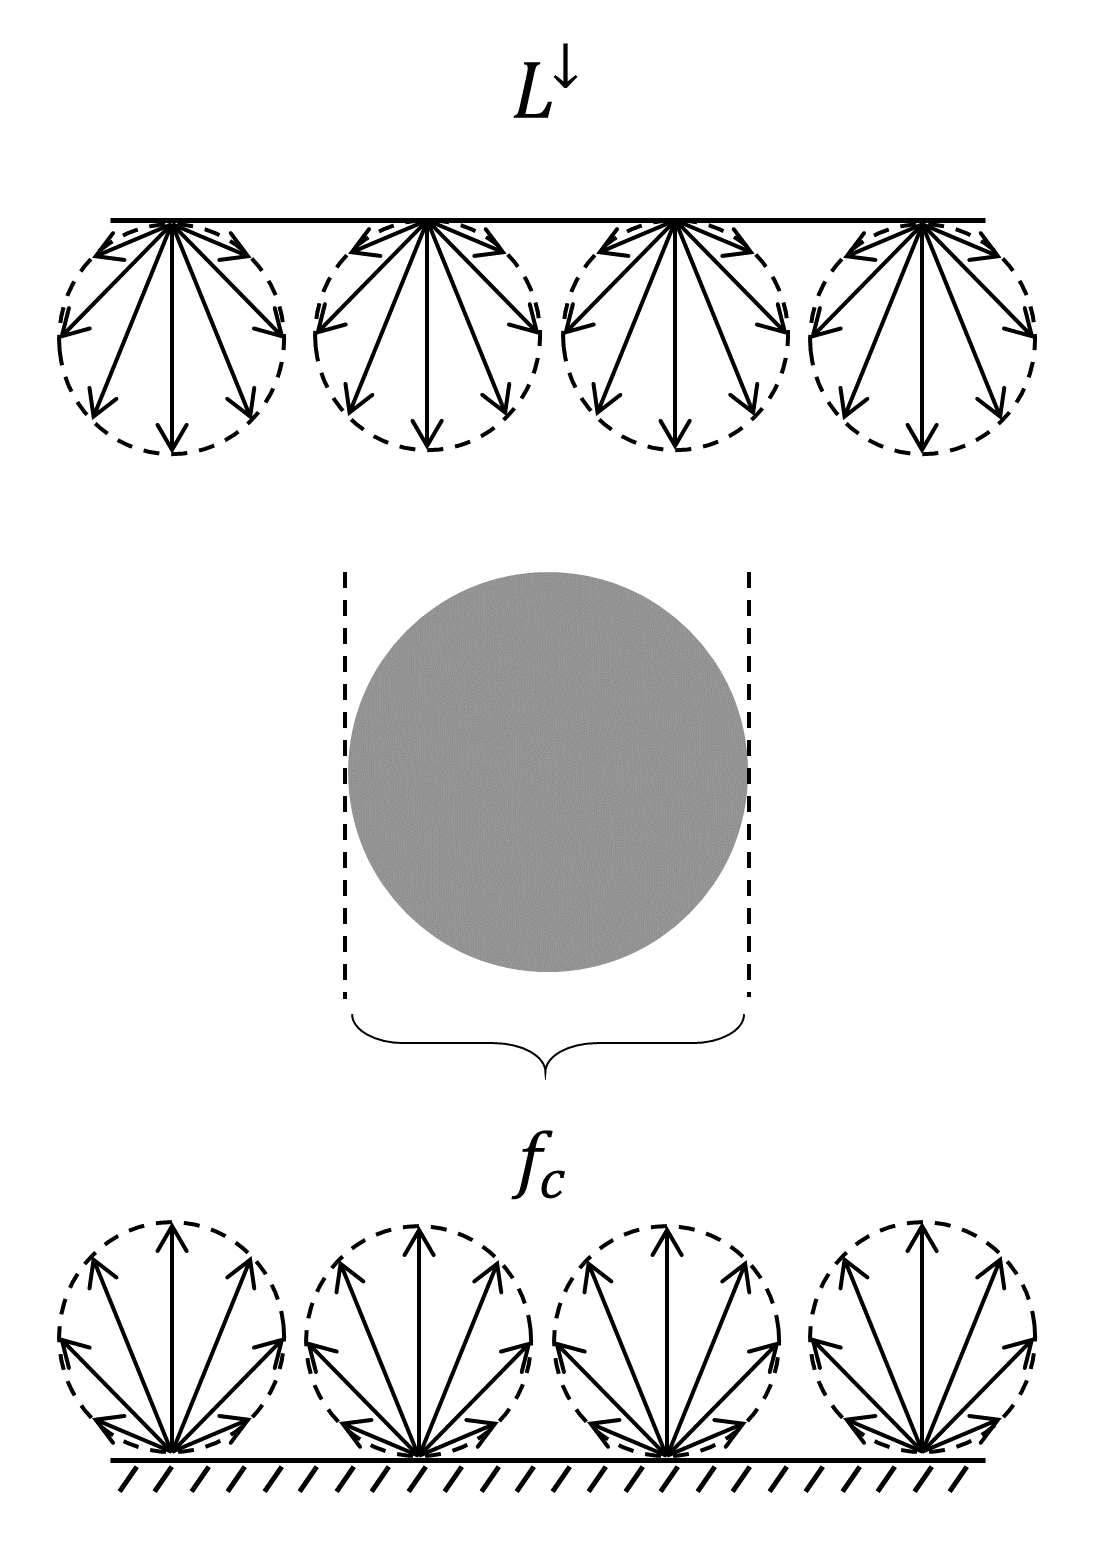
\includegraphics[width=0.5\textwidth]{Figures/辐射过程及辐射通量计算/单棵树冠长波辐射传输示意图.png}
\caption{三维长波辐射计算示意图(对于单棵树冠)}
\label{fig:单棵树冠长波辐射传输示意图}
\end{figure}
}
%
若采用一维长波辐射传输方式进行计算,则到达地面的大气长波辐射量即为$f_c\left(1-\varepsilon_v\right)L^\downarrow+\left(1-f_c\right)L^\downarrow$。
但实际上,由于长波辐射是朝各个方向发射的,一般认为各向均一(类似模式对短波漫射入射辐射假设),能到达树冠表面(或称为阴影)的长波辐射并不完全等同于其覆盖率(垂直投影面积)$f_c$,
简单的计算公式可以表示为:
\begin{equation}
S=\int_{2 \pi} \frac{\cos \theta}{\pi} \cdot \frac{f_{c}}{\cos \theta} \cdot d \Omega=2 f_{c}
\end{equation}
上式中$\cos{\theta}/\pi$为入射角度为$\theta$时的辐射强度,$f_c/\cos{\theta}$为此时的树冠阴影面积(地面投影),
总的阴影面积计算为$2f_c$。到达地面的大气长波辐射量即为:
\begin{equation}
S\left(1-\varepsilon_{v}\right) L ^\downarrow+(1-S) L ^\downarrow
\end{equation}
与一维不同之处是$f_c$替换成了$S$。当植被比较稀疏时,
$f_c\rightarrow0$,$S\rightarrow2$,同上述单棵树冠情况一样;
当植被比较致密时,$f_c\rightarrow1$,$S\rightarrow1$,同一维情形。
对从地面发射的长波辐射,其情况同向下大气长波辐射一样,在稀疏情况下,植被能截获更多的长波辐射。
下面我们对一层植被(植被覆盖度为$f_c$)进行整个长波辐射传输过程推导。植被冠层向下的长波辐射计算为:
\begin{equation}
\begin{aligned} 
L_{v} ^\downarrow &=S\left(1-\varepsilon_{v}\right) L ^\downarrow+(1-S) L ^\downarrow+f_{c} \varepsilon_{v} \sigma T_{v}^{4} \\ 
  &=\left(S-S \varepsilon_{v}+1-S\right) L ^\downarrow+f_{c} \varepsilon_{v} \sigma T_{v}^{4} \\ 
  &=\left(1-S \varepsilon_{v}\right) L ^\downarrow+f_{c} \varepsilon_{v} \sigma T_{v}^{4} 
\end{aligned}
\end{equation}
地面向上的长波辐射(包括自身发射和反射部分)计算为:
\begin{equation}
L_{g} ^\uparrow=\left(1-\varepsilon_{g}\right) L_{v} ^\downarrow+\varepsilon_{g} \sigma T_{g}^{4}
\end{equation}
地面的净长波辐射为:
\begin{equation}
{L_{g}}=\varepsilon_{g} L_{v} ^\downarrow -\varepsilon_{g} \sigma T_{g}^{4}
\end{equation}
植被净辐射通量为:
\begin{equation}
\begin{aligned} {L_{v}} &=-S \varepsilon_{v} L ^\downarrow-S \varepsilon_{v} L_{g} 
    ^\uparrow+2 f_{c} \varepsilon_{v} \sigma T_{v}^{4} \\ 
    &=-S \varepsilon_{v} L ^\downarrow-S 
    \varepsilon_{v}\left(1-\varepsilon_{g}\right)\left(1-S \varepsilon_{v}\right) L^\downarrow \\ 
    &\mathrel{\phantom{=}} -S \varepsilon_{v}\left(1-\varepsilon_{g}\right) f_{c} \varepsilon_{v} \sigma T_{v}^{4}+S
     \varepsilon_{v} \varepsilon_{g} \sigma T_{g}^{4}+2 f_{c} \varepsilon_{v} \sigma T_{v}^{4} \\ 
     &=\left[2-S \varepsilon_{v}\left(1-\varepsilon_{g}\right)\right] f_{c} \varepsilon_{v} 
     \sigma T_{v}^{4}-S \varepsilon_{v}\left[1+\left(1-\varepsilon_{g}\right)\left(1-S \varepsilon_{v}\right)\right]
      L ^\downarrow+S \varepsilon_{v} \varepsilon_{g} \sigma T_{g}^{4} \end{aligned}
\end{equation}
植被层顶向上的长波辐射计算为:
\begin{equation}
\begin{aligned} L_v ^\uparrow=&(1-S) L_{g} ^\uparrow+S\left(1-\varepsilon_{v}\right) L_{g} 
    ^\uparrow+f_{c} \varepsilon_{v} \sigma T_{v}^{4} \\=&\left(1-S \varepsilon_{v}\right) L_{g}
     ^\uparrow+f_{c} \varepsilon_{v} \sigma T_{v}^{4} \\=&\left(1-S \varepsilon_{v}\right)\left(1-\varepsilon_{g}\right)\left(1-S \varepsilon_{v}\right) L^\downarrow \\
      & \quad +\left(1-S \varepsilon_{v}\right)\left(1-\varepsilon_{g}\right) f_{c} \varepsilon_{v} \sigma T_{v}^{4}+\left(1-S \varepsilon_{v}\right) 
      \varepsilon_{g} \sigma T_{g}^{4}+f_{c} \varepsilon_{v} \sigma T_{v}^{4} \end{aligned}
\end{equation}
以上计算还需要考虑植被温度变化所带来的长波辐射量的改变,具体到$L_v^\downarrow$增加$4f_c\varepsilon_v\sigma T_v^3\Delta T_v$,${L_{g}}$增加$\varepsilon_{g} \Sigma 4 f_{c} \varepsilon_{v} \sigma T_{v}^{3} \Delta T_{v}$,$L_v ^\uparrow$增加$4 f_{c} \varepsilon_{v} \sigma T_{v}^{3} \Delta T_{v}+(1-\varepsilon_{g}) 4 f_{c} 
\varepsilon_{v}(1-\varepsilon_{v}) \sigma T_{v}^{3} \Delta T_{v}$。

将以上逻辑应用到之前描述的三层植被中,如图~\ref{fig:三层植被长波辐射传输示意图} 所示。
从计算示意图来看,稍显复杂,因为需要计算每两层之间的辐射传输量,其与短波辐射类似,具有一定规律。
%
{
\begin{figure}[htbp]
\centering
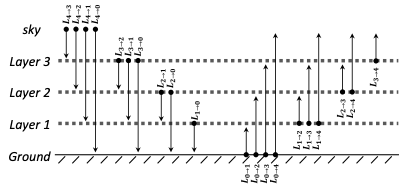
\includegraphics[width=0.8\columnwidth]{Figures/辐射过程及辐射通量计算/三层植被长波辐射传输示意图.png}
\caption[三层植被长波辐射传输示意图]{三层植被长波辐射传输示意图。4:天空,0:地面,1-3为植被层次,$L_{4 \rightarrow 3}$表示大气到达第三层植被的长波辐射,其他同}
\label{fig:三层植被长波辐射传输示意图}
\end{figure}
}
%

从天空下行的长波辐射到达每一层的辐射量为:
\begin{equation}
\begin{aligned} L_{4 \rightarrow 3} &=S_{3} L^\downarrow \\ L_{4 \rightarrow 2} &=\left(1-S_{3}\right) S_{2} L^\downarrow 
    \\ L_{4 \rightarrow 1} &=\left(1-S_{2}-S_{3}+S_{2} S_{3}\right) S_{1} L^\downarrow \\ 
    L_{4 \rightarrow 0} &=\left(1-S_{1}-S_{2}-S_{3}+S_{1} S_{2}+S_{1} S_{3}+S_{2} S_{3}-S_{1} S_{2} S_{3}\right) L^\downarrow \end{aligned}
\end{equation}
上式中,$S_n$表示第$n$层的阴影(等于太阳辐射传输中入射漫射辐射植被阴影)。从第3层植被向下到达各层的辐射量为:
\begin{equation}
\begin{aligned}
L_{3 \rightarrow 2} &=S_{2}\left(L_{3 \downarrow}+L_{3}\right) \\[1ex]
L_{3 \rightarrow 1} &=\left(1-S_{2}\right) S_{1}\left(L_{3 \downarrow}+L_{3}\right) \\[1ex]
L_{3 \rightarrow 0} &=\left(1-S_{1}-S_{2}+S_{1} S_{2}\right)\left(L_{3 \downarrow}+L_{3}\right)
\end{aligned}
\end{equation}
上式中$L_3 ^\downarrow$为从第3层植被向下穿透的长波辐射,$L_3$为第3层植被自身发射的长波辐射。
同理,从第2层植被及第1层植被向下到达各层的辐射量分别为:
\begin{equation}
\begin{aligned}
L_{2 \rightarrow 1} &=S_{1}\left(L_{2 \downarrow}+L_{2}\right) \\[1ex] 
L_{2 \rightarrow 0} &=\left(1-S_{1}\right)\left(L_{2 \downarrow}+L_{2}\right) \\[1ex]
L_{1 \rightarrow 0} &=L_{1 \downarrow}+L_{1}
\end{aligned}
\end{equation}
将以上的表达式经过简单整理,向下达到每一层的辐射量可以写成矩阵相乘的形式:
\begin{equation}
\boldsymbol{L}_{\rm dn}=\left(\begin{matrix}L_{1\downarrow}+L_1&L_{2\downarrow}+L_2&L_{3\downarrow}+L_3&L^\downarrow\\
\end{matrix}\right)\left(\begin{matrix}a_{10}&&&\\a_{20}&a_{21}&&
    \\a_{30}&a_{31}&a_{32}&\\a_{40}&a_{41}&a_{42}&a_{43}\\\end{matrix}\right)
\end{equation}
上式中右边的系数矩阵为:
\begin{equation}
\left(\begin{matrix}1&&&\\1-S_1&S_1&&\\1-S_1-S_2+S_1S_2&{\left(1-S_2\right)S}_1&S_2&\\
    1-S_1-S_2-S_3+S_1S_2+S_1S_3+S_2S_3-S_1S_2S_3&\left(1-S_2-S_3+S_2S_3\right)S_1&
    \left(1-S_3\right)S_2&S_3\\\end{matrix}\right)    
\end{equation}  
上次空白处表示0。若一层有多种PFT,其$L_n$计算为:
\begin{equation}
L_{n}=\sum f_{ci} \varepsilon_{i} \sigma T_{vi}^{4}
\end{equation}
$L_{n\downarrow}$计算为:
\begin{equation}
\begin{aligned}
L_{3 \downarrow} &=\sum \frac{S_{3i}\left(1-\varepsilon_{3i}\right)}{S_{3}} L_{4 \rightarrow 3} \\[1ex]
L_{2 \downarrow} &=\sum \frac{S_{2 i}\left(1-\varepsilon_{2 i}\right)}{S_{2}}\left(L_{4 \rightarrow 2}+L_{3 \rightarrow 2}\right) \\[1ex]
L_{1 \downarrow} &=\sum \frac{S_{1 i}\left(1-\varepsilon_{1 i}\right)}{S_{1}}\left(L_{4 \rightarrow 1}+L_{3 \rightarrow 1}+L_{2 \rightarrow 1}\right)
\end{aligned}
\end{equation}
上式中$S_{ni}$表示第$n$层植被PFT $i$的阴影面积,$\frac{\sum{S_{ni}\left(1-\varepsilon_{ni}\right)}}{S_n}$为每一层的属性,$\varepsilon_{ni}$为单独PFT属性。
先算$L_{3\downarrow}$,然后计算$L_{2\downarrow}$(需要$L_3$的计算结果),接着计算 $L_{1\downarrow}$,容易计算得到:
\begin{equation}
L_{v} ^\downarrow=L_{4 \rightarrow 0}+L_{3 \rightarrow 0}+L_{2 \rightarrow 0}+L_{1 \rightarrow 0} \text {, 即 } \boldsymbol{L}_{\rm dn}[1]
\end{equation}
\begin{equation}
L_{g} ^\uparrow =\left(1-\varepsilon_{g}\right) L_{v} ^\downarrow+\varepsilon_{g} \sigma T_{g}^{4}
\end{equation}
从土壤向上发射的辐射$L_g ^\uparrow $到达每一层植被的计算类似大气长波的向下传输:
\begin{equation}
\begin{aligned}
L_{0 \rightarrow 1} &=S_{1} L_{g} ^\uparrow\\[1ex]
L_{0 \rightarrow 2} &=\left(1-S_{1}\right) S_{2} L_{g} ^\uparrow \\[1ex]
L_{0 \rightarrow 3} &=\left(1-S_{1}-S_{2}+S_{1} S_{2}\right) S_{3} L_{g} ^\uparrow \\[1ex]
L_{0 \rightarrow 4} &=\left(1-S_{1}-S_{2}-S_{3}+S_{1} S_{2}+S_{1} S_{3}+S_{2} S_{3}-S_{1} S_{2} S_{3}\right) L_{g}^\uparrow
\end{aligned}
\end{equation}
从第1层植被向上到达各层的辐射量为:
\begin{equation}
\begin{aligned}
L_{1 \rightarrow 2} &=S_{2}\left(L_{1 \uparrow}+L_{1}\right) \\[1ex]
L_{1 \rightarrow 3} &=\left(1-S_{2}\right) S_{3}\left(L_{1 \uparrow}+L_{1}\right) \\[1ex]
L_{1 \rightarrow 4} &=\left(1-S_{2}-S_{3}+S_{2} S_{3}\right)\left(L_{1 \uparrow}+L_{1}\right)
\end{aligned}
\end{equation}
上式中$L_1\uparrow$为从第1层植被向上穿透的长波辐射,$L_1$为第1层植被自身发射的长波辐射。同理,从第2层植被及第3层植被向上到达各层的辐射量分别为:
\begin{equation}
\begin{aligned}
L_{2 \rightarrow 3} &=S_{3}\left(L_{2 \uparrow}+L_{2}\right) \\[1ex]
L_{2 \rightarrow 4} &=\left(1-S_{3}\right)\left(L_{2 \uparrow}+L_{2}\right) \\[1ex] 
L_{3 \rightarrow 4} &=L_{3 \uparrow}+L_{3} 
\end{aligned}
\end{equation}
将以上的表达式经过简单整理,向上到达每层的辐射量同样可以写成矩阵相乘的形式:
\begin{equation}
\boldsymbol {L}_{\rm up}=\left(\begin{matrix}L_g ^\uparrow &L_{1\uparrow}+L_1&L_{2\uparrow}+L_2&L_{3\uparrow}+L_3\\\end{matrix}
\right)\left(\begin{matrix}a_{01}&a_{02}&a_{03}&a_{04}\\&a_{12}&a_{13}&a_{14}\\
&&a_{23}&a_{24}\\&&&a_{34}
\\\end{matrix}\right)
\end{equation}
上式中右边的系数矩阵为:
\begin{equation}
\left(\begin{matrix}S_1&\left(1-S_1\right)S_2&\left(1-S_1-S_2+S_1S_2\right)S_3&
    1-S_1-S_2-S_3+S_1S_2+S_1S_3+S_2S_3-S_1S_2S_3\\&S_2&{\left(1-S_2\right)S}_3&1-S_2-S_3+S_2S_3\\
    &&S_3&1-S_3\\&&&1\\\end{matrix}\right)   
\end{equation}
同理,
\begin{equation}
L_v ^\uparrow=L_{0 \rightarrow 4}+L_{1 \rightarrow 4}+L_{2 \rightarrow 4}+L_{3 \rightarrow 4}, \text { 即 } \boldsymbol{L}_{\rm up}[4]
\end{equation}
到达每一层植被(或地面、天空)的辐射即为:
\begin{equation}
\boldsymbol L=\boldsymbol L_{\rm dn}+\boldsymbol L_{\rm up}
\end{equation}
单个PFT所吸收的辐射量为:
\begin{equation}
{L_{v i}}=\frac{S_{ni}}{S_{n}} \varepsilon_{ni} L_{* \rightarrow n}-2 f_{ci} \varepsilon_{i} \sigma T_{vi}^{4}
\end{equation}
$L_{\ast\rightarrow n}$即为到达每一层的辐射,即为$L[n]$。注意上式是整个归一化面积上的计算结果,
或者说是在整个土壤patch上的计算,单位面积上的吸收还需要除以各自的覆盖度$f_{ci}$。

在湍流迭代求解植被温度时,我们还需要用到$L_{vi}$对自身温度的偏导数。PFT吸收的长波辐射来自自身发射的部分可计算如下: \\
%
对于第1层植被:
\begin{equation}
f_{ci} \varepsilon_{vi} \sigma T_{vi}^{4}\left(1-\varepsilon_{g}\right) S_{i} \varepsilon_{vi}
\end{equation}
对于第2层植被:
\begin{equation}
f_{ci} \varepsilon_{vi} \sigma T_{vi}^{4}\left[\left(1-S_{1}\right)+\sum S_{1 i}\left(1-\varepsilon_{1 i}\right)\right]
\left(1-\varepsilon_{g}\right)\left[\left(1-S_{1}\right)+\sum S_{1 i}\left(1-\varepsilon_{1 i}\right)\right] S_{i} \varepsilon_{vi}
\end{equation}
对于第3层植被:
\begin{equation}
\begin{aligned} 
    f_{c i} \varepsilon_{v i} \sigma T_{v i}^{4}\left[\left(1-S_{1}-S_{2}+S_{1} S_{2}\right)+
    \sum S_{2 i}\left(1-\varepsilon_{2 i}\right)\left[\left(1-S_{1}\right)+\sum S_{1 i}\left(1-\varepsilon_{1 i}\right)\right]\right.\\[1ex] 
    \left.+\left(1-S_{2}\right) \sum S_{1 i}\left(1-\varepsilon_{1 i}\right)\right]\left(1-\varepsilon_{g}\right)\left[\left(1-S_{1}-S_{2}+S_{1} S_{2}\right)\right.\\[1ex] 
    +\sum S_{1 i}\left(1-\varepsilon_{1 i}\right)\left[\left(1-S_{2}\right)+\sum S_{2 i}\left(1-\varepsilon_{2 i}\right)\right] \\[1ex] 
    \left.+\left(1-S_{1}\right) 
    \sum S_{2 i}\left(1-\varepsilon_{2 i}\right)\right] S_{i} \varepsilon_{v i}
\end{aligned}
\end{equation}
%\begin{equation}
%\begin{aligned} 
%    f_{ci} \varepsilon_{vi} \sigma T_{vi}^{4}
%    \left[\left(1-S_{1}-S_{2}+S_{1}S_{2}\right)+\sum S_{2i}\left(1-\varepsilon_{2i}\right)
%    \left[\left(1-S_{1}\right)+\sum S_{1i}\left(1-\varepsilon_{1i}\right)\right]\\
%    +\left(1-S_{2}\right) \sum S_{1i}\left(1-\varepsilon_{1i}\right)\right]
%     \left(1-\varepsilon_{g}\right)
%     \left[\left(1-S_{1}-S_{2}+S_{1} S_{2}\right)\\
%      &+\sum S_{1i}\left(1-\varepsilon_{1i}\right)\left[\left(1-S_{2}\right)+\sum S_{2i}\left(1-\varepsilon_{2i}\right)\right] \\ 
%      +\left(1-S_{1}\right) \sum S_{2i}\left(1-\varepsilon_{2i}\right)\right] S_{i} \varepsilon_{vi}
 %\end{aligned}
%\end{equation}
同时需要考虑自身发射的长波辐射$-2f_{ci}\varepsilon_{vi}\sigma T_{vi}^4$。
$L_{vi}$对于叶温的变化率为以上两者之和对$T_{vi}$求导,同时需要除以$f_{ci}$ (转换成在单位面积上的值)。 
植被温度最后一次迭代的改变所包含的能量分配到$L_v ^\downarrow$增加
$\Sigma4f_{ci}\varepsilon_{vi}\sigma T_{vi}^3\Delta T_{vi}$,$L_{g}$增加$\varepsilon_g\Sigma4f_{ci}\varepsilon_{vi}\sigma T_{vi}^3\Delta T_{vi}$,$L_v ^\uparrow$增加$\Sigma 4 f_{ci} \varepsilon_{vi} \sigma T_{vi}^{3} \Delta T_{vi}+\left(1-\varepsilon_{g}\right) \Sigma 4 f_{ci} \varepsilon_{vi}\left(1-\varepsilon_{vi}\right) \sigma T_{vi}^{3} \Delta T_{vi}$。


\section{短波吸收辐射通量}\label{短波吸收辐射通量}
\begin{mymdframed}{代码}
本章节对应代码为\texttt{MOD\_NetSolar.F90}。
\end{mymdframed}

在计算得到地表反照率后,地表总的太阳短波辐射通量(包括地面和植被)吸收为:
\begin{equation}
S_{v g}=S_{vis,dir}\left(1-\alpha_{vis,dir}\right)+S_{vis,dif}\left(1-\alpha_{vis,dif}\right)+
S_{nir,dir}\left(1-\alpha_{nir,dir}\right)+S_{nir,dif}\left(1-\alpha_{nir,dif}\right)
\end{equation}
其中等式右边$S$表示太阳短波在不同波段(可见光$vis$、近红外$nir$)和直射/漫射时($dir$/$dif$)的辐射通量。阳叶、阴叶辐射通量吸收分别为:
\begin{equation}
S_{s u n}=S_{vi s, dir} s_{s u n, vi s, dir}+S_{vis, dif} s_{s u n, vis, dif}+S_{ni r, dir} s_{s u n, ni r, dir}+S_{nir, dif} s_{s u n, nir, dif}
\end{equation}
\begin{equation}
S_{s h a}=S_{vis, dir} s_{sun,vis,dir}+S_{vis, dif} s_{sun,vis,dif}+S_{ni r, dir} s_{sun,nir,dir}+S_{nir, dif} s_{sun,nir,dif}
\end{equation}
植被总的吸收辐射通量为:
\begin{equation}
S_{v}=S_{s u n}+S_{s h a}
\end{equation}
地面的吸收辐射通量为:
\begin{equation}\label{eq:sg}
S_{g}=S_{v g}-S_{s u n}-S_{s h a}
\end{equation}
单位面积阳叶、阴叶有效光合辐射吸收通量为:
\begin{equation}
\text{PAR}_{sun} =S_{vis, dir} s_{sun, vis, dir}+S_{vis, dif} s_{sun, vis, dif}
\end{equation}
\begin{equation}
\text{PAR}_{sha} =S_{vis, dir} s_{sha, vis, dir}+S_{vis, dif} s_{sha, vis, dif}
\end{equation}


\section{长波净辐射通量}\label{长波净辐射通量}
\begin{mymdframed}{代码}
本章节对应代码包含于\texttt{MOD\_GroundTemperature.F90, MOD\_LeafTemperature.F90}。
\end{mymdframed}

地表发射的长波辐射是基于斯蒂芬-玻尔兹曼定律来计算。
当为土壤时,地面发射率$\varepsilon_g$设置为0.96;对于冰川,设置为0.97。

对于裸土覆盖情况,地面的长波净辐射通量计算为:
\begin{equation}
L_{g}=\varepsilon_{g} L ^\downarrow
\end{equation}
其中$L ^\downarrow$表示大气向下长波辐射通量。

对于一维植被覆盖情况,植被长波透射率计算为:
\begin{equation}
\tau_{v}=\exp \left(-\frac{\text{LAI+SAI}}{\bar{\mu}}\right)
\end{equation}
植被发射率(即吸收率)计算为:
\begin{equation}
\varepsilon_{v}=1-\exp \left(-\frac{\text{LAI+SAI}}{\bar{\mu}}\right)=1-\tau _v
\end{equation}
其中$\rm SAI$表示植被茎面积指数。植被的长波净辐射通量计算为:
\begin{equation}
L_{v}=\varepsilon_{v}\left(L ^\downarrow-2 \sigma T_{v}^{4}+\varepsilon_{g} \sigma T_{g}^{4}\right)
\end{equation}
其中$T_v$表示叶片温度,$T_g$表示土壤表层温度,$\sigma$表示斯蒂芬-玻尔兹曼常数。地面净长波辐射吸收为:
\begin{equation}\label{eq:lg1}
L_g= \tau_{v} L ^\downarrow \varepsilon_g - \varepsilon_{g} \sigma T_{g}^{4}
\end{equation}

注意,以上的计算并未考虑植被向下长波辐射到达地面后的反射部分,即假设全部被地面吸收。在新版本中,考虑一次土壤反射,然后被植被吸收,其计算表达式为:
\begin{equation}
L_{v}=\varepsilon_{v}\left(L ^\downarrow-2 \sigma T_{v}^{4}+\varepsilon_{g} \sigma T_{g}^{4}\right)+\left(1-\varepsilon_{g}\right)\left(1-\varepsilon_{v}\right) \varepsilon_{v} L ^\downarrow+\left(1-\varepsilon_{g}\right) \varepsilon_{v}^{2} \sigma T_{v}^{4}
\end{equation}
地面净长波辐射计算为:
\begin{equation}\label{eq:lg2}
L_{g}=\left(\tau_{v} L ^\downarrow  + \varepsilon_{v} \sigma T_{v}^{4} \right) \varepsilon_{g} - \varepsilon_{g} \sigma T_{g}^{4}
\end{equation}
以上计算是针对一维植被情景,对于三维植被净长波辐射计算见章节~\ref{三维植被长波辐射传输}。

\section{太阳天顶角}\label{太阳天顶角}
\begin{mymdframed}{代码}
本章节对应代码为\texttt{MOD\_OrbCoszen.F90}。
\end{mymdframed}

太阳天顶角的余弦$\mu$的表达式为
\begin{equation}
\mu= \sin(\phi)\sin(\delta)−\cos(\phi)\cos(\delta)\cos(h)
\end{equation}
%
其中$h$为太阳时角,$\delta$是黄赤交角,$\phi$是纬度(北半球为正;单位均为弧度),太阳时角$h$的表达式为:
\begin{equation}
h=2\pi d+\theta
\end{equation}
$d$是儒略日 (Julian Day),$\theta$是经度(格林威治子午线以东为正)。计算$\delta$需要的轨道参数有地球的倾斜角$\varepsilon$、地球的离心率$e$、近日点相对于春分点的经度$\widetilde{\omega}$。黄赤交角$\delta$计算式为:
\begin{equation}
\delta= \sin^{−1}[\sin(\epsilon) \sin(\lambda)]
\end{equation}
%
$\varepsilon$为地球倾斜角,设置为 \num{0.409214646},单位弧度。$\lambda$为地球实际的经度(单位弧度),其计算从春分开始逆时针计算($\lambda$在春分点为0),其表达式为:
\begin{equation}
\lambda = \lambda_{m0} + \left( 2e - \frac{1}{4}e^{3} \right)\sin\left( \lambda_{m} - \widetilde{\omega} \right) + \frac{5}{4}e^{2}\sin\left[2\left( \lambda_{m} - \widetilde{\omega} \right)\right] + \frac{13}{12}e^{3}\sin\left[3\left( \lambda_{m} - \widetilde{\omega} \right)\right]
\end{equation}
%
$\lambda_{m0}$是春分时的平均经度,设置为 \num{-3.2625366e-2}。$e$设置为 \num{1.672393084e-2}。$\widetilde{\omega}$设置为 \num{4.92251015}。平均经度$\lambda_{m}$计算为:
%
\begin{equation}
\lambda_{m} = \lambda_{m0} + \frac{2\pi\left( d - d_{ve} \right)}{365}
\end{equation}
%
其中\(d_{ve} = 80.5\)是春分时儒略日(3月21日中午)。
%\end{辐射过程及辐射通量计算}
